% !TEX TS-program = pdflatex


\documentclass{lncs/llncs}

\usepackage[T1]{fontenc}
%\usepackage{geometry}                % See geometry.pdf to learn the layout options. There are lots.
%\geometry{a4paper}                   % ... or a4paper or a5paper or ...
%\geometry{landscape}                % Activate for for rotated page geometry
%\usepackage[parfill]{parskip}    % Activate to begin paragraphs with an empty line rather than an indent
\usepackage{graphicx}
\usepackage{DotArrow}

%\usepackage{amsfonts}
%\usepackage{fancyhdr}
%\usepackage{cite}
%\usepackage{ifthen}
%\usepackage{amssymb}
%\usepackage{fancyhdr}
%\usepackage{pifont}
\usepackage{stmaryrd}
\usepackage{mathtools,mathpartir}
\usepackage{proof}
%\usepackage{setspace}
%\usepackage{indentfirst}
\usepackage{amsmath,amssymb,amscd,mathrsfs}
\DeclareGraphicsRule{.tif}{png}{.png}{`convert #1 `dirname #1`/`basename #1 .tif`.png}
\usepackage{epsfig,color,subfigure,enumitem}
\newcommand{\TODO}[1]{\textcolor{red}{\textbf{[TODO:#1]}}}
\newcommand{\NOTE}[1]{\textcolor{blue}{\textbf{[NOTE:#1]}}}
\newcommand{\ERIC}[1]{\textcolor{blue}{#1}}
\newcommand{\LUDO}[1]{\textcolor{green}{#1}}
\newcommand{\RAB}[1]{\textcolor{magenta}{#1}}
\newcommand{\coloncolon}{{:\hspace{-.2ex}:}}
\makeatletter
\newcommand{\raisemath}[1]{\mathpalette{\raisem@th{#1}}}
\newcommand{\raisem@th}[3]{\raisebox{#1}{$#2#3$}}
\makeatother

\usepackage{macrospNets}


%\usepackage[math]{cellspace}
%\setlength\cellspacetoplimit{ 37pt}
%\setlength\cellspacebottomlimit{18pt}

\pagestyle{plain}

% addition to the mathpartir package for red dotted rules,
% that we use for open-transitions


%\newtheorem{theorem}{Theorem}[section]
\newtheorem{prop}[theorem]{Proposition}
%\newtheorem{corollary}[theorem]{Corollary}
%\newtheorem{lemma}[theorem]{Lemma}
\newtheorem{algorithm}[theorem]{Algorithm}
%\newtheorem{remark}[theorem]{Remark}
%\newtheorem{definition}[theorem]{Definition}
%\newtheorem{example}[theorem]{Example}
%\newtheorem{problem}[theorem]{Problem}
%\newtheorem{proof}[theorem]{Proof}


\title{More equivalences for Open pNets\thanks{This work was partially 
funded by the Associated Team FM4CPS
  between INRIA and ECNU, Shanghai}}
\author{ Ludovic Henrio\inst{1}  \ \ \  Eric Madelaine\inst{1,2} \ \ \ Min Zhang\inst{3}}
\institute{Univ. of Nice Sophia Antipolis, CNRS, UMR 7271, 06900 Sophia Antipolis, France
	\and INRIA Sophia Antipolis M\'edit\'erann\'ee, BP 93, 06902 Sophia Antipolis, France
\and Shanghai Key Laboratory of Trustworthy Computing, ECNU, China}
\date{}                                           % Activate to display a given date or no date

                          % Activate to display a given date or no date


\begin{document}

\maketitle

%\section{}
%\subsection{}


\begin{abstract}
  Strong bisimulation allows to compare open systems described using the pNets model.
  In practice, as happens in process algebras, it is too strong, and
  we need to define some coarser relations, taking into account
  invisible or internal moves.

  Open pNets have a notion of \emph{synchronised actions}
  generalizing the usual internal actions (e.g. $\tau$ of CCS, or $i$
  in Lotos).

  We use this notion to define an equivalence relation similar to
  the classical \emph{weak bisimulation}, and study its properties...

  refinement preorders ?

  Algorithms ?

  Which significant (small) use-case ?

\end{abstract}


\section{Status and TODO list}
Improve and simplify Tr2

notation guards in  SV




\section{Introduction}

\ERIC{imported from FORTE'16, but many of these works also had weak
  version... we need to have another look}

In the nineties, several 
works extended the basic behavioural models based on labelled
transition systems to address value-passing or parameterised systems, using
various symbolic encodings of the
transitions~\cite{deSimone85,Larsen87,HennessyLin:TCS95,Linconcur96}. 
In \cite{Linconcur96}, H.M. Lin addressed value-passing calculi, for which he
developed a symbolic behavioural semantics, and proved algebraic properties.
Separately J. Rathke~\cite{HennessyRathke:TCS98} defined another
symbolic semantics for 
a parameterised broadcast calculus, together with strong and weak bisimulation
equivalences, and developed a symbolic model-checker based on a tableau
method for these processes. 30 years later, no
practical verification approach and no verification platform are
using this kind of approaches to provide proof methods for
value-passing processes or open process expressions. 

\paragraph{Contribution}

\paragraph{Related works}



\paragraph{Structure.}


\section{Notations}

\subsubsection{Syntax and Notations}
\TODO{copy pasted -- rearrange + move?}

In the following definitions, we extensively use indexed structures
(maps) over some countable indexed sets. The indices will usually be
integers, bounded or not. Such an indexed family is denoted as
follows: $a_i^{i\in I}$ is a family of elements $a_i$ indexed over the
set $I$. Such a family
is equivalent to the mapping $(i\mapsto a_i)^{i\in I}$, and we will also use mapping 
notations to manipulate indexed sets.
To specify the set over which the structure is indexed, 
indexed structures are always denoted with an exponent of the form $i\in I$
(arithmetic only appears in the indexes if necessary).
Consequently, $a_i^{i\in I}$ defines first $I$ the set over which the
family is indexed, and then $a_i$ the elements of the family.

For example $a^{i\in\{3\}}$ is
the mapping with a single entry $a$ at index $3$; exceptionally, such mappings with
only a few entries will also be denoted $(3\mapsto a)$.
%The operation  $A[j \mapsto a]$ updates the value associated to $j$ in map $A$ so that 
%it 
%now corresponds to $a$. 
When this is not ambiguous, we shall use abusive vocabulary and
notations for sets, and typically write ``indexed set over I'' when  
formally we should speak of multisets, and ``$x\in
A_i^{i\in I}$'' to mean $\exists i\in I.\, x=A_i$.
An empty family is denoted $[]$. % (it can be defined as $a_i^{i\in\emptyset}$).
To simplify equations, an indexed set can be denoted $\set{M}$
instead of $M_l^{l\in L}$ when $L$ is irrelevant.

$\uplus$ is the disjoint operator on sets. We extend it to  disjoint union  of indexed 
sets defined by the merge of the 
two sets provided they are indexed on disjoint families.
The elements
of the union of two indexed sets are then accessed by using an index of one of the two
joined families.
We suppose here that disjoint unions are always well defined; this
requires to choose disjoint  
indices in the definition of the component system (e.g. name of
methods of different interfaces).
We denote $y\gets x$ a substitution. The application of the substitution is denoted
$\subst{y\gets x}$, the operation replaces in a term all occurrences 
of the term $y$ by the term $x$ (note that the absence of binders makes this operation 
trivial).

\section{Parameterised Networks (pNets): definition}
\label{section:pnets}

This section introduces pNets and the notations we will use in
this paper. Then it gives the formal definition of pNet structures,
together with an operational semantics for open pNets.

pNets are tree-like structures, where the leaves are either
\emph{parameterised labelled transition systems (pLTSs)}, expressing the
behaviour of basic processes, or \emph{holes}, used as placeholders
for unknown processes, of which we only specify the set of possible
actions, this set is named the \emph{sort}.
Nodes of the tree (pNet nodes) are synchronising artifacts, using a
set of \emph{synchronisation vectors} that express the possible
synchronisation between the parameterised actions of a subset of the
sub-trees.

%\LUDO{introduce magic op}
%$\CreateISet{a}{i}$ creates a single entry indexed set $(i\mapsto a)$ \emph{but only if 
%$a$ is not already an indexed set.}

%\smallskip\noindent
\paragraph*{Notations.}
We extensively use indexed structures
over some countable indexed sets, which are equivalent to mappings over
the countable set. % . The indexes will usually be
% integers, bounded or not. Such an indexed family is
%denoted
%follows:
$a_i^{i\in I}$
%, or equivalently  $(i\mapsto a_i)^{i\in I}$
denotes a family of elements $a_i$ indexed over the
set $I$. % Such a family
% is equivalent to the mapping $(i\mapsto a_i)^{i\in I}$.
% To specify the set over which the structure is indexed,
% indexed structures are always denoted with an exponent of the form $i\in I$
% (arithmetic only appears in the indexes if necessary).
$a_i^{i\in I}$ defines both $I$ the set over which the family is
indexed (called \emph{range}), and $a_i$ the elements of the family.
E.g., $a^{i\in\{3\}}$ is the mapping with a single entry $a$ at index
$3$ ; abbreviated $(3\mapsto a)$ in the following.
When this is not
ambiguous, we shall use notations for sets, and typically write
``indexed set over I'' when formally we should speak of multisets, and
write $x\in a_i^{i\in I}$ to mean $\exists i\in I.\, x=a_i$.  An empty
family is denoted $\emptyset$. We
denote classically with an overline -- $\overline{a}$  -- a family when the indexing set 
is
not meaningful.  $\uplus$ is the disjoint union on
indexed sets.

\paragraph*{Term algebra.}
Our models rely on a notion of parameterised actions, that are
symbolic expressions using data types and variables. As our model aims
at encoding the low-level behaviour of possibly very different
programming languages, we do not want to impose one specific algebra
for denoting actions, nor any specific communication mechanism. So we
leave unspecified the constructors of the algebra that will allow building
expressions and actions. Moreover, we use a generic {\em action interaction}
mechanism, based on (some sort of) unification between two or more action
expressions, to express various kinds of communication or
synchronisation mechanisms.

\def\Talg{\mathcal{T}_{\Sigma,\P}}
Formally, we assume the existence of a term algebra $\Talg$,
where $\Sigma$ is the signature of the data and action constructors,
and $\P$ a set of variables. Within $\Talg$, we distinguish a set of
data expressions $\mathcal{E}_\P$, including a set of boolean
expressions $\mathcal{B}_{\P}$ ($\mathcal{B}_{\P}\subseteq\mathcal{E}_\P$).
On top of $\mathcal{E}_\P$ we build the action algebra
$\mathcal{A}_\P$, with $\mathcal{A}_P\subseteq\mathcal{T}_\P,
\mathcal{E}_P\cap\mathcal{A}_P=\emptyset$;
naturally action terms will use data expressions as subterms.
To be able to reason about the data flow between pLTSs, we
distinguish \emph{input variables} of the form $?x$ within terms; the function
$\vars(t)$ identifies the set of variables in a term
$t\in\AlgT$, and $iv(t)$ returns its input variables.
Action algebras can encode naturally usual point-to-point message passing calculi (using 
$a(?x_1,...,?x_n)$ for inputs, $a(v_1,..,v_n)$ for outputs), but it also allows
for more general mechanisms, like gate negociation in Lotos, or broadcast
communications. 



\subsection{The (open) pNets Core Model}
\label{section:pNets}


A pLTS is a labelled transition system with variables; variables can be
manipulated, defined, or accessed inside states, actions, guards, and
assignments. Without loss of generality and to simplify the formalisation, we suppose 
here that 
variables are local to each 
state: each state has its set of variables disjoint from the others. Transmitting 
variable values from one state to the other can be done by explicit assignment. 
%Similarly, to simplify the management of variables and without loss of expressivity, we 
%suppose that transitions looping to the same state does not do assignments.
Note that we make no assumption on finiteness of the set of states nor
on finite branching of the transition relation.

We first define the set of actions a pLTS can use, let $a$
range over action labels, $\symb{op}$ are operators, and $x_i$ range over
variable names. Action terms are:
\[
\begin{array}[l]{rcl@{\quad}p{5.5cm}}
  \alpha\in\AlgA&::=&a(p_1,\ldots,p_n)&\text{action terms}\\
  p_i&::=& ?x~|~\symb{Expr}&\text{parameters (input variable or expression)}\\
  \symb{Expr}&::=& \symb{Value}~|~x~|~\symb{op}(\symb{Expr}_1,..,\symb{Expr}_n)&\text{Expressions}
\end{array}
\]
The input variables in an action term are those marked with a
$\symb{?}$.
We additionally suppose that each input variable does not
appear somewhere else in the same action term:
$p_i=?x\Rightarrow\forall j\neq i.\, x\notin \vars(p_j)$

\begin{definition}[pLTS]
\label{pLTS}
A pLTS is a tuple
$\pLTS\triangleq\mylangle S,s_0, \to\myrangle$ where:
\begin{itemize}
\item[$\bullet$]
$S$ is a set of states.
\item[$\bullet$]
$s_0 \in S$ is the initial state.
%\item[$\bullet$]
 %Variables in
%$\iv(\alpha)$ are assigned by the action, other variables can be assigned
%by the additional assignments.
\item[$\bullet$] $\to \subseteq S \times L \times S$ is the transition relation and 
$L$ is the set of labels of the form
$\langle \alpha,~e_b,~(x_j\!:= {e}_j)^{j\in J}\rangle$,
where $\alpha \in\AlgA$ is a parameterised action, $e_b \in
\AlgB$ is a guard, and the variables $x_j\in P$
are assigned the expressions $e_j\in \AlgE$.
If 
$s \xrightarrow{\langle \alpha,~e_b,~(x_j\!:= {e}_j)^{j\in
		J}\rangle} s'\in \to $ then 
% REMOVED BECAUSE USELESS: $\iv(\alpha)\!\subseteq\! \vars(s')$, 
		$\vars(\alpha)\backslash \iv(\alpha)\!\subseteq\! \vars(s)$, 
		$\vars(e_b)\!\subseteq\! \vars(s)\cup\vars(\alpha)$, and
		$\forall j\!\in\! J .\,\vars(e_j)\!\subseteq\! \vars(s)\cup\vars(\alpha)\land 
		x_j\!\in\!\vars(s')$. %,  and $s= s'\Rightarrow J=\emptyset$. 
\end{itemize}
\end{definition}

Now we define
pNet nodes, as constructors for hierarchical behavioural structures.
A pNet has a set of sub-pNets that can be either pNets or pLTSs, and a
set of Holes, playing the role of process parameters.

A composite pNet consists of a set of sub-pNets exposing
a set of actions, each of them synchronising actions in each of
the sub-pNets. The synchronisation between global actions and
internal actions is given by  \emph{synchronisation vectors}: a
synchronisation vector synchronises one or several internal actions, and
exposes a single resulting global action.
Actions involved at the pNet level (in the synchronisation vectors) do
not need to distinguish  input 
variables. Action terms for pNets are defined as follows:
\[\begin{array}[l]{rcl@{\quad}l}
  \alpha\in \AlgAS &::=&a(Expr_1,\ldots,Expr_n)
\end{array}
\]

We now define the structure of pNets, the following definition relies on the definition 
of holes, leaves and sorts provided below in Definition~\ref{def-sortholeleave}.

\begin{definition}[pNets]\label{def-pnets}
A pNet is a hierarchical structure where leaves are pLTSs and holes:\\
$\pNet\triangleq \pLTS~|~\mylangle \pNet_i^{i\in I}, \Sort_j^{j\in J}, \symb{SV}_k^{k\in 
K}\myrangle$
where
\begin{itemize}
\item[$\bullet$] $I \in \I$ is the set over which sub-pNets are indexed.
\item[$\bullet$] $\pNet_i^{i\in I}$ is the family of sub-pNets.
%  $\pNet_i^{i\in I}$ is a family of sub-pNets where $I\in\I_\P$ is the set over which sub-pNets are indexed.

\item[$\bullet$] $J\!\in\!\I_\P$ is a set of indexes, called \emph{holes}.
$I$ and $J$ are \emph{disjoint}: $I\!\cap\! J=\emptyset$,  $I\!\cup\! J\neq\emptyset$
\item[$\bullet$] $\Sort_j \subseteq \AlgAS$ is a set of action terms, denoting the 
\emph{sort} of
hole $j$.

\item[$\bullet$] $\symb{SV}_k^{k\in K}$ is a set of
  synchronisation vectors ($K\in\I_\P$). $\forall k\!\in\! K,
  \symb{SV}_k\!=\!\alpha_{l}^{l\in I_k \uplus J_k}\to\alpha'_k\,|\,e_k$ where
  $\alpha'_k\in \mathcal{A}_\P$, $I_k\subseteq I$, $J_k\subseteq J$,
  $\forall i\!\in\!
  I_k.\,\alpha_{i}\!\in\!\Sort(\pNet_i)$,  $\forall j\!\in\!
  J_k.\,\alpha_{j}\!\in\!\Sort_j$, and $\vars(\alpha'_k)\subseteq \bigcup_{l\in I_k\uplus 
  J_k}{\vars({\alpha_l})}$. The global action of a vector $\symb{SV}_k$ is
$\alpha'_k$. $e_k \in \AlgB$ is a guard associated to the vector 
$\vars(e_k)\subseteq \bigcup_{l\in I_k\uplus J_k}{\vars({\alpha_l})}$.


\end{itemize}
\end{definition}

The preceding definition relies on the auxiliary functions defined below:

\begin{definition}[Sorts, Holes, Leaves of pNets]\label{def-sortholeleave}
  \begin{itemize}
  \item The sort of a pNet is its signature, i.e. the set of actions it can
perform. In the definition of sorts, we do not need to distinguish
input variables (that specify the dataflow within LTSs), so for
computing LTS sorts, we use a substitution operator\footnote{$\subst{y_k\gets x_k}^{k\in K}$ is the parallel substitution 
operation.} to remove the
\emph{input marker} of variables. Formally:
\[
\begin{array}{l}
\Sortop(\mylangle S,s_0, \to\myrangle) = \{\alpha\subst{x \gets ?x| 
x\in\symb{iv}(\alpha)}|s \xrightarrow{\langle \alpha,~e_b,~(x_j\!:= {e}_j)^{j\in
    J}\rangle} s'\in \to \} \\
\Sortop(\mylangle \overline{\pNet}\!, %\pNet_i^{i\in I}, \Sort_j^{j\in J}
\overline{\pNet}\!,
\overline{\symb{SV}}\myrangle)
=\{\alpha' |\, \overline{\alpha}%\alpha_j^{j\in J_k}
\to\alpha'\in\set{\symb{SV}}\}
\end{array}
\]

\item
The set of holes of a pNet is defined inductively; the sets of holes
in a pNet node and its subnets are all disjoint:
  \[\begin{array}{l}
\Holes(\mylangle S,s_0, \to\myrangle) \!=\! \emptyset\\
\Holes(\mylangle \pNet_i^{i\in I}\!,\Sort_j^{j\in J}\!, \overline{\symb{SV}}\myrangle) 
=J\uplus{\displaystyle \bigcup_{i\in 
I}\Holes(\pNet_i)}\\
\forall i\in I.\, \Holes(\pNet_i)\cap J=\emptyset\\
\forall i_1,i_2\in I.\,i_1\neq i_2\Rightarrow  \Holes(\pNet_{i_1})\cap\Holes(\pNet_{i_2})=\emptyset
\end{array}\]
\item
The set of leaves of a pNet is the set of all pLTSs occurring in the structure, defined 
inductively as:
\[\begin{array}{l}
\Leaves(\mylangle S,s_0, \to\myrangle) \!=\!\{\mylangle S,s_0, \to\myrangle\}\\
\Leaves(\mylangle \pNet_i^{i\in I}\!,%Sort_j^{j\in J}
\overline{\Sort}\!, \overline{\symb{SV}}\myrangle) = {\displaystyle \biguplus_{i\in 
I}\Leaves(\pNet_i)\uplus\{i\mapsto \pNet_i|\pNet_i \text{ is a }\pLTS\}}
\end{array}\]
\end{itemize}
\end{definition}



A pNet $Q$ is \emph{closed} if it has no hole: $\Holes(Q)=\emptyset$; else it
is said to be \emph{open}.


\begin{figure}[t]
%\begin{minipage}{\linewidth}

  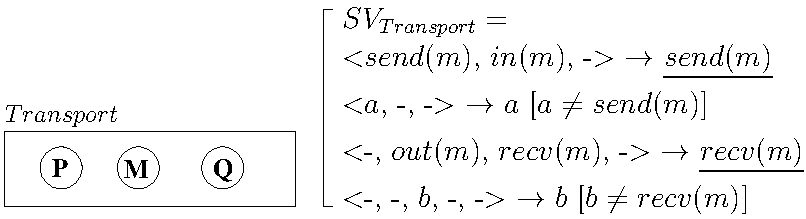
\includegraphics[width=7cm]{XFIG/Transport}
  \hspace{0.5cm}
 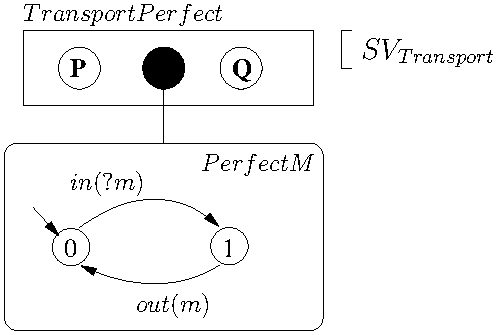
\includegraphics[width=4.5cm]{XFIG/TransportSpec}
  \caption{Schema and specification of the protocol }  \label{schema:enable-pnets}
%\end{minipage}
  \vspace{1cm}
%\begin{minipage}{6cm}
  \centerline{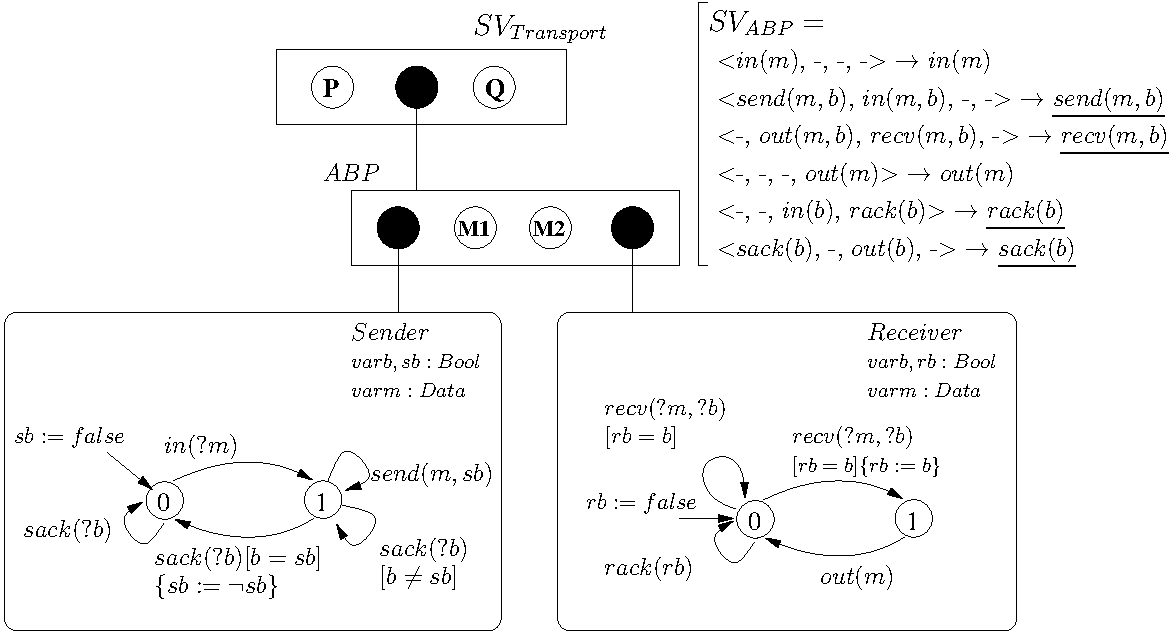
\includegraphics[width=11cm]{XFIG/ABPSchema}}
  \caption{Composed pNet with the ABP protocol}  \label{schema:enable-composed}
%\end{minipage}

\end{figure}





\section{Operational Semantics for Open pNets}
\label{section:op-semantics}


The semantics of open pNets will be defined  as an open automaton. An open
automaton is an automaton where each transition composes transitions of several LTSs with
action of some holes, the transition occurs if some predicates hold, and can involve a 
set of state modifications.
%\TODO{adopt a uniform notation for open transitions, almost each instance has a 
%different 
%notation! I suggest p,l,pr,po using \{\} for p,l,po as they are sets}
\begin{definition}[Open transitions]
	\label{def:OpenTransitions}
	An \emph{open transition} over a set  $(S_i,s_{0 i}, \rightarrow_i)^{i\in
	I}$ of LTSs, a
	set $J$ of holes with sorts $\Sort_j^{j\in J}$, and a set of states $\mathcal{S}$ is 
	a structure of the form:	
	\begin{mathpar}
	\inferrule*[myfraction=\reddottedrule]
	{\{s_i~{\xrightarrow{a_i}}_i ~s_i^{\prime}\}^{i\in I},
		\{\xrightarrow{b_j}_j\}^{j\in J}, \Pred, \Post}
	{s \OTarrow {v}s'}
	\end{mathpar}
	Where $s, s'\in\mathcal{S}$ and for all
        $i\in I$, $s_i{\xrightarrow{a_i}}_i s_i^{\prime}$ is a transition of the
	LTS $(S_i,s_{0 i}, \rightarrow_i)$, and $\xrightarrow{b_j}_j$
        is a transition of the hole $j$, for any action $b_j$ in the
        sort $\Sort_j$. $v$ is a variable denoting the resulting action
        of this open transition. \Pred\ is a predicate 
	over the different variables of the
	terms, labels, and states $s_i$, $b_j$, $s$, $v$. \Post\ is a set of equations that 
	hold \emph{after the open transition}, they are represented as a substitution of the 
	form $\{x_k\gets e_k\}^{k\in K}$ 
	where $x_k$ are variables of $s'$, $s'_i$, and $e_k$ are expressions over the other 
	variables of the open transition.
\end{definition}


\begin{example}\emph{An open-transition.}
  \label{OT:enable-composed}
  The \texttt{EnableCompL} pNet of Fig. \ref{schema:enable-composed} has 2 controllers and 2 holes. One of its possible open-transition is:

 \smallskip
 $  OT_2  = \openrule{
                       0 \xrightarrow{\delta}_{C_3} 1 ~~
                            0 \xrightarrow{l}_{C_4} 0  ~~                 
                            \xrightarrow{\delta(x4)}_P ~~
                            \xrightarrow{accept(x4)}_Q 
                      }
  %  {\ostate{00} \xrightarrow{\underline{\delta(x1)}} \ostate{10}}
    {A1_0 \OTarrow{\underline{\delta(x4)}} A1_1}
  $
\end{example}


\begin{definition}[Open automaton]
	\label{def:open-automaton}
	An \emph{open automaton} is a structure\\ $A =
	<\LTS_i^{i\in I},J,\mathcal{S},s_0,\mathcal{T}>$ where:
	\begin{itemize}
		\item[$\bullet$]  $I$ and $J$ are  sets of indices,
		\item[$\bullet$]  $\LTS_i^{i\in I}$ is a family of LTSs,
		\item[$\bullet$]   $\mathcal{S}$ is a set of states and $s_0$ an initial state
		among $\mathcal{S}$,
		\item[$\bullet$] $\mathcal{T}$ is a set of open transitions and for each
		$t\in \mathcal{T}$ there exist $I'$, $J'$ with $I'\subseteq I$, $J'
		\subseteq J$, such that $t$ is an open transition over $\LTS_i^{i\in I'}$, $J'$,
		and  $\mathcal{S}$.
		
	\end{itemize}
\end{definition}
	

%
%Then the semantics of a pNet is characterized by a set of {\em open
%transitions}, where the hypotheses on process parameters are
%replaced by 1) transitions of the pLTSs at the leaves, and 2) formal
%hypotheses on the transitions of the holes. A {\em predicate} is used
%to relate the parameters and names appearing in the actions of the
%leaves and the holes involved in the rules, but also appearing in  the resulting action.

We define states of open pNets as tuples of states, where we denote tuples
in structured states as $\triangleleft\ldots\triangleright$ for distinguishing tuple 
states from other tuples.
\begin{definition}[States of open pNets]\label{def-states}
  A state of an open pNet is a tuple (not necessarily finite) of the
  states of its leaves.

  For any pNet p, let $\Leaves(p) = \mylangle S_i,{s_i}_0, \to_i\myrangle^{i \in L}$ be 
  the set of pLTS at its leaves,
  then $States(p) = \{\triangleleft s_i^{i\in L}
  \triangleright| \forall i\in L. s_i \in S_i\}$.
A pLTS being its own single leave:
  $States(\mylangle S,s_0, \to\myrangle) = \{\triangleleft s \triangleright| s \in S\}$.

The initial state is defined as:
$InitState(p) = \triangleleft {{s_i}_0}^{i\in L}  \triangleright$.
\end{definition}



%% \begin{example} \emph{State of a pNet}
%%   The states of pNet \texttt{EnableCompL} are:
%%   $\triangleleft 00 \triangleright, \triangleleft 10 \triangleright, \triangleleft 11 \triangleright$
%% \end{example}

\paragraph{Predicates:}
Let
$\mylangle\overline{\pNet},\overline{\Sort},\overline{\symb{SV}}\myrangle$
be a pNet. Consider a synchronisation vector $\symb{SV}\in \overline{\symb{SV}}$. We 
define a
predicate $\Pred$ relating
the actions of the involved sub-pNets and the resulting actions. This predicate verifies:
\[\Pred_{\symb{sv}}(SV, a_i^{i\in I}, b_j^{j\in J}, v)\Leftrightarrow \bigg(
\begin{array}{l}
\exists {(a'_i)}^{i\in I},
{(b'_j)}^{j\in J},v'.\, SV={(a'_i)}^{i\in I}, {(b'_j)}^{j\in J}\rightarrow v' | e_b
\\~~\land
\forall i\in I.\, a_i=a'_i\land \forall j \in J.\, b_j=b'_j \land v=v' \land e_b
\end{array} \bigg)\]

Somehow, this predicate entails a verification of satisfiability in the sense that if the 
predicate $\Pred_{\symb{sv}}$ is not satisfiable, then the transition associated with the 
synchronisation will not occur in the considered state. 


In any other case (if the action families do not match or if there is no valuation of
variables such that the above formula can be ensured) the predicate is undefined.

This definition is not constructive but it is easy to build the predicate constructively
by brute-force unification of the sub-pNets
actions with the corresponding vector actions, possibly followed by a simplification
step.


We build the semantics of open pNets as an open automaton where LTSs are the pLTSs at
the leaves of the pNet structure, and the states are given by 
Definition~\ref{def-states}. The open transitions first
 project the global state into states of the leaves, then apply
pLTS transitions on these states, and compose them with the sort of the holes. %The pNet
%structure does not appear in the open-automaton, only the
%set of Holes and the set of Leaves.
The semantics   regularly instantiates \emph{fresh} variables, and uses a
\emph{clone} operator that clones a term replacing each variable with a
fresh one.


\begin{definition}[Operational semantics of open pNets]
	\label{def:operationalSemantics}
	The semantics of a pNet $p$ is an open automaton $A = <Leaves(p),Holes(p),States(p),InitState(p),
	\mathcal{T}>$ where $\mathcal{T}$ is the smallest set of open transitions		satisfying the rules below:
%	\begin{itemize}
%		\item $J$ is the set of holes: $Holes(p)= J$. 
		%  \item $\overline{L}^L = Leaves(p), \overline{H}^J = Holes(p)$
%		\item ${\mathcal{S}} = States(p)$ and $s_0 = InitState(p)$
%		\item $\mathcal{T}$ is the smallest set of open transitions		satisfying the rules below:
%	\end{itemize}
	
	%% \TODO{ We should be careful here: after (re) reading "Huimin
	%% 	Lin, 'Symbolic Transition Systems with Assignements', Concur'96" I
	%% 	think handling assignments is not trivial, even for comparisons of pLTSs. }


	
	The rule for a pLTS  checks that the guard 
	is verified and transforms assignments into post-conditions:
	
	\begin{description}
		\item[{\bf Tr1:}]
		$\inferrule
		{ s \xrightarrow{\langle \alpha,~e_b,~(x_j\!:= {e}_j)^{j\in
					J}\rangle} s'\in \to  }
		{ \mylangle  S,s_0, \to \myrangle
			\models
			\inferrule*[myfraction=\reddottedrule]
			{\{s \xrightarrow{\alpha} s'\} ,\emptyset ,
			e_b,\left\{x_j\gets e_j\right\}^{j\in J}}
			{\ostate{s} \OTarrow{\alpha} \ostate{s'}}
		}
		$\LUDO {removed a ${}_p$ that was not bound}
	\end{description}
%	Note that this note is greatly simplified by the fact that variables are local to 
%	thread; introducing global state variables or accepting loops to the same 
%	state would 
%	require to reason 
%	on the scope of 
%	each variables, and to introduce additional variables to handle the several occurence 
%	of the same pLTS variable in the predicates. Indeed the constraints on pLTS 
%	transitions 
%	ensure that the same variable never appears both on the left and on the right of the 
%	equations of a predicate.
	
	The second rule deals with pNet nodes: for each possible
	synchronisation vector applicable to the rule subject, the premisses
	include one {\em open transition} for each sub-pNet involved, one possible
	{\em action} for each Hole involved, and the predicate relating these
	with the resulting action of the vector.
	A key to understand this rule is that the open transitions are
	expressed in terms of the leaves and holes of the pNet structure,
	i.e. a flatten view of the pNet: e.g. $L$ is the index set of the
	Leaves, $L_m$ the index set of the leaves of one subnet indexed $m$, so all $L_m$
	are disjoint subsets of $L$. Thus the states in the open transitions,
	at each level, are tuples including states of all the
	leaves of the pNet, not only those involved in the chosen
	synchronisation vector.
	\LUDO{now with two cases of induction} \LUDO{Why I'm and not Im?}
	\begin{description}
		\item[{\bf Tr2:}]
	\end{description}
	
	\noindent
    $\inferrule
    {k\!\in\! K \\SV_k \!=\! \alpha_m^{m \in I\uplus J} \!\to\! 
    \alpha' |e_b \\
    	Leaves(\mylangle \pNet_i^{i\in I'}, \overline{\Sort}, \symb{SV}_k^{k\in 
    	K}\myrangle) \!=\! \pLTS_l^{l\in L} \\    	
    	\forall m\!\!\in\!\! I. 	
    {\left(\begin{array}{l}
	{\pNet_m \models\inferrule*[myfraction=\reddottedrule]
    	{\{s_{i}\xrightarrow{a_{i}}_i s_{i}'\}^{i\in I_m^\prime},
    	\{\xrightarrow{b_{j}}_j\}^{j\in J'_m}, \Pred_m, \Post_m}
    	{\ostate{s_{i}^{i \in L_m}} \OTarrow {v_m}
    		\ostate{(s_i^\prime)^{i\in L_m}}}\lor }\\
		{ \pNet_m 
    	 \models
    	\inferrule*[myfraction=\reddottedrule]
    	{\{s_m \xrightarrow{v_m} s_m'\},\emptyset, \Pred_m, \Post_m}
    	{\ostate{s_m} \OTarrow {v_m}
    		\ostate{s_m'}} \land I'_m=\{m\} \land J'_m=\emptyset}
\end{array}\right)}\\
    	%\land
    	%Leaves(\pNet_m) = \overline{\pLTS}^{L_k})  	
     J' = \biguplus_{m\in I}\!\! J'_m \uplus J 	\\
    	\Pred = \bigwedge_{m\in I}\!\! \Pred_m \land
    	\Pred_{\symb{sv}}(SV_k,v_m^{m\in I},b_j^{j\in J},v)\\ 
    		I' = \biguplus_{m\in I}\!\! I_m'
    	\\\forall i\in	L\backslash I'.\,s'_i=s_i \\
    {\tt fresh}(\alpha_m,\alpha',b_j,v) 
    }
    {\mylangle \pNet_i^{i\in I'}, \overline{\Sort}, \symb{SV}_k^{k\in K}\myrangle
    	\models
    	{\inferrule*[myfraction=\reddottedrule]
    		{\{s_i\xrightarrow{a_i}_i s_i^{\prime}\}^{i\in I^\prime},
    		\{\xrightarrow{b_j}_j\}^{j\in J^\prime}, \Pred, \uplus_{m\in I_k} 
    		\Post_m}
    		{\ostate{s_i^{i\in L}} \OTarrow {v}
    			\ostate{(s_i^\prime)^{i\in L}}}
    	}
    }
    $
	\medskip
%        \TODO{may be explain how $\Pred(SV,a_i^{i\in I_k},b_j^{j\in
%            J_k},v)$ is built ? You mean more than what is written on previous page????}
	%%    \TODO{I have tentatively added the sort constraint on hole actions, that was
	%%not included in the first version... I'm unsure whether this is the best place to
	%%include it, because it may change the decidability conditions on predicates}
	
\end{definition}
%

\begin{example} \emph{Using the operational rules to compute
    open-transitions}
  In Fig. \ref{usingrules:OT2} we show the deduction tree used to construct and prove the 
  open transition $OT_2$ of \texttt{EnableCompL} (see example page \pageref{OT:enable-composed}).
  The rule uses TR1 for the $\delta$ transition of $C_3$, for the $l$ transition of $C_4$, then combines the result using the $a_4$ vector of the bottom pNet node, and the $\underline{\delta(x)}$ vector of the top node.
  
\begin{figure}[tb]
\begin{mathpar}
  \small
  \inferrule
    {\inferrule
        {0 \xrightarrow {\delta}_{C_3} 1}
        {C_3
          \models
            \openrule{
              0 \xrightarrow {\delta}_{C_3} 1,\,
              \{\xrightarrow{\delta(x_1)}_P\},\,
              v_1=\delta(x_1)}
                      {\ostate{0}\OTarrow{v_1}\ostate{1}}
        }\\
%      \sm{fresh}v         \\
      \inferrule%*[right={L_1}]
        {
%          \sm{fresh}{a_Q} \\
          \inferrule
              {0 \xrightarrow{l}_{C_4} 0}
              % {\ostate{0}\xrightarrow{l}\ostate{0}}
              {C_4
                \models
                \openrule{
                      0 \xrightarrow l_{C_4} 0,\,
                      \sm{Pred}_{C_4}}
                      {\ostate{0}\OTarrow{l}\ostate{0}}
              }
        }
        {
          \textrm{Q>>R}\models
              \openrule
                  { 0 \xrightarrow {l}_{C_4} 0,\,
                    \{\xrightarrow{acc(x_2)}_Q\},\,
                    \ v_2=acc(x_2)
                  }
                  {\ostate{0}\OTarrow{v_2}\ostate{0}}
        }   
    }
    {
     \textrm{P>>(Q>>R)}
     \models
     \openrule
         { 0 \xrightarrow{\delta}_{C_3} 1, \\ 0 \xrightarrow{l}_{C_4} 0,\\
           \{\xrightarrow{\delta(x)}_P,\,\xrightarrow{acc(x)}_Q\}, \\
            a_3=v_1 \wedge v=a_3 \wedge x_1=x_2
           }
         {\ostate{00} \OTarrow{v} \ostate{10}}
      }\vspace{-4ex}
\end{mathpar}
  \caption{Proof of transition $OT_2$ (with interaction of processes $P$ and $Q$) for ``P>>(Q>>R)''}
  \label{usingrules:OT2}
\end{figure}

\end{example}

Note that while the scenario above is expressed as a single
instantiation of the possible behaviours, the constructions below are
kept symbolic, and each open-transition deduced expresses a whole family of
behaviours, for any possible values of the variables.

\paragraph{Variable management.}
The variables in each synchronisation vector are considered local:
for a given pNet expression, we must have fresh local variables for
each occurrence of a vector (= each time we instantiate rule
Tr2). Similarly the state variables of each copy of a
given pLTS in the system, must be distinct, and those created for each
application of Tr2 have to be fresh and all distinct. 
This will be implemented within the open-automaton generation algorithm,
e.g. using name generation using a global counter as a suffix.



\subsection{Computing and using open automata}
In this section we present a simple algorithm to construct the open
automaton representing the behaviour of an open pNet, and we prove that
under reasonable conditions this automaton is finite.

\TODO{Eric: refine the algorithm description}

\begin{algorithm}[Behavioural semantics of open pNets: Sketch]
This is a standard residual algorithm over a set of open-automaton
states, but where transitions are open transitions
constructively ``proven'' by deduction trees.

1) Start with a set of unexplored states containing the initial state
of the automaton, and an empty set of explored states.

2) While there are unexplored states:

2a) pick one state from the unexplored set and add it to the explored
set. From this state
build all possible deduction trees by application of the structural
rules Tr1 and Tr2, using all \ERIC{applicable} combinations
of synchronisation vectors.

2b) For each of the obtained deduction trees, extract the resulting
open-transition, with its predicate and \Post\ assignments by exploring the structure of 
the pNet.

2c)
\ERIC{The predicate is submitted to Z3 for checking satisfiability. If it is NOT stisfiable, the resulting OT is discarded. This will minimize the number of
resulting transitions, and potentialy prune the search-space.}

2d)
\ERIC{Optionally, simplify the predicate by eliminating the unnecessary intermediate variables, that were produced as fresh local variables of synchronisation vectors, and fresh result variables of intermediate OTs. In the resulting predicate the only significant variables are :\\
- the input variables of pLTS transitions\\
- the actions of holes\\
- the result action at toplevel.}

For each open-transition,  add the transition in the outgoing transitions of
the current state, and add the
resulting state in the unexplored set if it is not already in the
explored set.

%3) this ends with the "while" from step 2, when we have no more
%unexplored set.
\end{algorithm}



Given an open-pNet
with finite synchronisation sets, finitely many leaves and
holes, and each pLTS at leaves having a finite number of states and
(symbolic) transitions, has a finite automaton (see \ref{Forte}).

  \TODO{Eric: define ``elimination of intermediate variables ?'' it
    transforms the predicates, it is not an
    ``equivalence'' transformation, rather some sort of
    abstraction... Does it change the satisfiability ?}

%% \begin{theorem}[Finiteness of open-automata.]\\
%% Given an open pNet $\mylangle \overline{\pNet},\overline{S}, \symb{SV}_k^{k\in K}\myrangle$ with leaves $pLTS_i^{i\in L}$ and holes $Hole_j^{j\in
%%   J}$, if the sets $L$ and $J$ are finite, if the synchronisation vectors of all pNets 
%%   included in  $\mylangle \overline{\pNet},\overline{S}, \symb{SV}_k^{k\in K}\myrangle$ 
%%   are finite, and if
%% $\forall i \in L.\, finite{(states(pLTS_i))} \text{ and } pLTS_i$
%% has a finite number of state variables, then Algorithm 1 terminates
%% and produces an open automaton 
%% $\mathcal{T}$ with finitely many states and transitions.


% Given an open pNet $\mylangle \overline{\pNet},\overline{S}, \symb{SV}_k^{k\in
%     K}\myrangle$ with leaves $pLTS_i^{i\in L}$ and holes $Hole_j^{j\in
%   J}$,
% build its semantics as in algorithm 1.

% We have:

% $$ finite{(L)} \land finite{(J)} \land \forall i \in L finite{(\{s_i\})}
%   \to finite{(\mathcal{T})}$$
% \end{theorem}


\TODO{Eric: full result of the tool execution on the running example}


\section{Bisimulation}
\label{section:bisimulation}

	Now we use our symbolic operational semantics to define a notion of
	strong (symbolic) bisimulation. Moreover this equivalence is decidable whenever we 
	have some
	decision procedure on the predicates of the action algebra.


%% , that we prove compatible with the
%% composition of open pNets. \TODO{do we really know this ?}

The equivalence we need is a strong bisimulation between
pNets having exactly the same Holes with the same sorts, but using a
flexible matching 
between open transition, to accommodate comparisons between pNet
expressions with different architectures.
 We name it FH-bisimulation,
 as a short cut for the ``Formal Hypotheses'' manipulated in the
 transitions, but also as a reference to the work of De Simone~\cite{deSimone85},
 that pioneered this idea.

Let $\mathcal{R}=\{(s,t|\Pred_{s,t})\}$ be a relation over the set $\mathcal{S}_1$ and 
$\mathcal{S}_2$ constrained by a predicate
More precisely, for any pair $(s,t)$, there is a 
   single
      $(s,t|\Pred_{s,t})\in\mathcal{R}$  stating that $s$ and $t$ are related 
      if $\Pred_{s,t}$ 
      is 
      true, i.e. the states are related when the variables in $s$ and $t$ verify the 
      predicate $\Pred_{s,t}$.
 FH-bisimulation is defined formally: 
 \begin{definition}[Strong FH-bisimulation]\label{def-FH-bisim} 

\noindent
\begin{minipage}{0.69\linewidth} 	Suppose that
   $A_1 = <\overline{\LTS_1},J,\mathcal{S}_1, s_0,
   \mathcal{T}_1>$ and $A_2 = <\overline{\LTS_2},J,\mathcal{S}_2,t_0, \mathcal{T}_2>$
   are open automata where the set
   of holes are equal 
   and of the same sort.  

 Then 
$\mathcal{R}$ is an FH-bisimulation iff for any  states
$s\in\mathcal{S}_1$ and $t\in\mathcal{S}_2$, $(s,t|\Pred_{s,t})\in\mathcal{R}$, we 
have
the following:
\end{minipage}
\hspace{2mm}
\begin{minipage}{0.30\linewidth}
	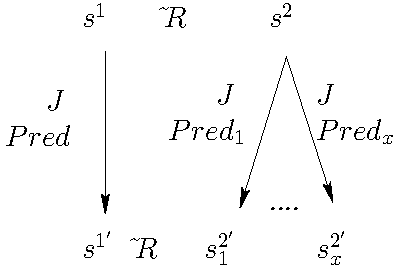
\includegraphics[width=\linewidth]{XFIG/Bisim}
	\TODO{J'ai ajoute les predicats. Il reste a dessiner la ``couverture'' si j'y arrive...}
\end{minipage}




 \begin{itemize}
 \item  For any open transition $OT$ in $\mathcal{T}_1$:
 \begin{mathpar}
     \inferrule*[myfraction=\reddottedrule]
         {\{s_i\xrightarrow{a_i}_i s'_i\}^{i\in I_1}, % , s_i,s'_i\in 
         %States(I_1)
           \{\xrightarrow{b_j}_j\}^{j\in J_1},\Pred_{OT},\Post_{OT}}
         {s \OTarrow {v} s'}

\end{mathpar}
 there exist open transitions $OT_x^{x\in X} \subseteq \mathcal{T}_2$:
 \begin{mathpar}
%    \left( fresh \ \overline{a_i}, \overline{b_j}, v_x.\ \
    \inferrule*[myfraction=\reddottedrule]
         {\{t_i\xrightarrow{a_{i x}}_i t_{i x}\}^{i\in I_{ x}},
           \{\xrightarrow{b_{j x}}_j\}^{j\in J_{x}}, \Pred_{OT_x},\Post_{OT_x}}
         {t \OTarrow {v_x} t_x}
%         \right)
\end{mathpar}
 such that  $\forall x, J_1=J_{x}, \exists \Pred_{s',t_x}. (s',t_x|\Pred_{s',t_x})\in 
 \mathcal{R}$; 
 and  \\
 $\Pred_{s,t} \land \Pred_{OT}\\
\hspace{1cm} \implies\!\!\! \bigvee_{x\in X}
   \left( \forall j. b_j=b_{jx}  \Rightarrow \Pred_{OT_x}
     \land v\!=\!v_x \land  
     \Pred_{s',t_x}\subst{\Post_{OT}}\subst{\Post_{OT_x}}\right)$
     %     \symb{Subst}(\Pred_{target_x}, \Post_{OT} o \Post_{OT_x})
     %     \right)$.

     \TODO{Eric: j'ai ajoute $\exists$ sur les predicats $\Pred_{s',t_x}$, qui n'etaient pas definis...}
     
 \item  and symmetrically any open transition from $t$ in $\mathcal{T}_2$ can be 
      covered by a set of transitions from $s$ in $\mathcal{T}_1$.
 \end{itemize}

% \TODO{Eric: il reste des petits bugs genre $s^{2'}_x$ plutot que
%   $s^{2}_x$}
 
%Where $\symb{Subst}(\Pred,\Post)$ is the parallel substitution of all
%assigned variables.
Two pNets are FH-bisimilar if there exist a relation between their associated 
automata that is an FH-bisimulation and their initial states are in the relation, i.e. 
the predicate associated to the relation between the initial states is true.
% \TODO{do we want formulas for this?}
 \end{definition}
Classically, $\Pred_{s',t_x}\subst{\Post_{OT}}\subst{\Post_{OT_x}}$
applies in parallel the  
substitutions $\Post_{OT}$ and $\Post_{OT_x}$ (parallelism is crucial
inside each $\Post$ set but $\Post_{OT}$ is independent from
$\Post_{OT_x}$), applying the assignments of the involved rules.



\medskip
If we assume that everything is finite (states and transitions in the
open automata, and the predicates in $\mathcal{R}$, then it is easy to
prove that it is decidable whether a relation is a 
FH-bisimulation, provided the logic of the predicates is decidable (see
\cite{henrio:Forte2016}). 






\begin{theorem}[Decidability of FH-bisimulation]
Let $A_1$ and $A_2$ be finite open automata
and $\mathcal{R}$ a relation over their states $\mathcal{S}_1$ and
$\mathcal{S}_2$ constrained by a finite set of predicates. Assume that
the predicates inclusion is decidable over  
the action algebra $\mathcal{A}_P$. Then it is decidable whether the relation 
$\mathcal{R}$ is a FH-bisimulation.
  
\end{theorem}




\section{Composability}

The main interest of our symbolic approach is to define a method to
prove properties directly on open structures, that will be preserved
by any correct instantiation of the holes. In this section we define a
composition operator for open pNets, and we prove that it preserves
FH-bisimulation. More precisely, one can define two preservation
properties, namely 1) when one hole of a pNet is filled by two bisimilar
other (open) pNets; and 2) when the same hole in two bisimilar pNets are
filled by the same pNet, in other words, composing a pNet with two
bisimilar contexts. The general case will be obtained by
transitivity of the bisimulation relation. We concentrate here on the
second property, that is the most interesting.



\begin{theorem}[FH-Bisimulation is an equivalence]\label{thm-equiv} Suppose $\mathcal{R}$ 
is an FH-bisimualtion. Then $\mathcal{R}$ is an equivalence, that is, $\mathcal{R}$ is 
reflexive, symmetric and transitive.

\end{theorem}



\begin{definition}[pNet composition]
	An open pNet: $\pNet = \mylangle \pNet_i^{i\in I}, \Sort_j^{j\in J}, 
	\overline{\symb{SV}}\myrangle$
 can be (partially) filled by providing  a pNets $\pNet'$ of the
	right sort to fill one of  its holes.	
	Suppose $j_0\in J$:
	%% \[\mylangle \pNet_i^{i\in I},S_j^{j\in J}, \symb{SV}_k^{k\in
	%%   K}\myrangle\left[(\pNet'_i)^{i\in L}\right]= \mylangle \pNet_i^{i\in
	%%   I}\left[(\pNet'_i)^{i\in L}\right]\uplus(\pNet'_i)^{i\in J\cap L},S_j^{j\in 
	%%J\setminus L},
	%% \symb{SV}_k^{k\in K}\myrangle
	%% \]
	\[\pNet\left[\pNet'\right]_{j_0}= \mylangle 
	\pNet_i^{i\in I}\uplus\{j_0\mapsto \pNet'\},\Sort_j^{j\in J\setminus \{j_0\}},
	\overline{\symb{SV}}\myrangle
	\]
\end{definition}


\begin{theorem}[Congruence]\label{thm-congr-eq}
	Consider an open pNet:
	$\pNet = \mylangle \pNet_i^{i\in I}, \Sort_j^{j\in J}, 
	\overline{\symb{SV}}\myrangle$.
	Let $j_0\in J$ be a hole. Let $Q$ and $Q'$ be two FH-bisimilar pNets such that 
	$\Sortop(Q)=\Sortop(Q')=\Sort_{j_0}$\footnote{Note that $\Sortop(Q)=\Sortop(Q')$ is 
	ensured by 
	strong bisimilarity.}. Then 
	$\pNet[Q]_{j_0}$ and 
	$\pNet[Q']_{j_0}$ are FH-bisimilar.
\end{theorem}

\begin{theorem}[Context equivalence]\label{thm-ctxt-eq}
	Consider two FH-bisimilar open pNets:
	$\pNet = \mylangle \pNet_i^{i\in I}, \Sort_j^{j\in J}, 
	\overline{\symb{SV}}\myrangle$ and 	$\pNet' = \mylangle {\pNet'}_i^{i\in I}, 
	\Sort_j^{j\in 
	J}, 	\overline{\symb{SV'}}\myrangle$ 
	(recall they must have the same holes to be bisimilar).
	Let $j_0\in J$ be a hole, and $Q$ be a pNet such that $\Sortop(Q)=\Sort_{j_0}$. Then 
	$\pNet[Q]_{j_0}$ and 
	$\pNet'[Q]_{j_0}$ are FH-bisimilar.
\end{theorem}

Finally, the previous theorems can be composed to state a general theorem about 
composability and FH-bisimilarity.
\begin{corollary}[Composability]
	Consider two FH-bisimilar pNets with an arbitrary number of holes, when replacing, 
	inside those two original pNets, a subset of the holes by FH-bisimilar pNets, we 
	obtain two FH-bisimilar pNets.
\end{corollary}
%
%In the following we use $\approx$ to denote equality modulo alpha conversion of free 
%variables. In practice, $x\approx y$ can be obtained if: $x=clone(a) \land y=clone(a)$.


\section{Weak bisimulation}

Weak symbolic bisimulation was introduced to relate transition systems
that have indistinguishable behaviour, with respect to some definition
of \emph{internal actions} that are considered local to some
subsystem, and consequently cannot be observed, nor used for
synchronisation with their context.
As the notions of invisible action varies in different contexts,
e.g. $tau$ in CCS, and $i$ in Lotos, we will rely here on some set of
\emph{internal actions} depending on a specific action
algebra. Naturally, an internal action cannot be synchronised with
actions of other systems in its environment. 

%% \TODO{we should understand if it make sense to distinguish invisible
%%   from synchronised actions: in the Forte paper we wrote ``using  as 
%% \emph{invisible actions} a subset of the
%% \emph{synchronised actions} defined in Section~\ref{section:pnets}''}.

%% Proving bisimulation properties on our hierarchical broadcast example
%% would take too much space for this paper. Moreover, interesting
%% properties of the HB example would rather be adequate for weak
%% bisimulation, and its large state-space would require some
%% tool-assistance, both for the generation of the open-automata and for
%% their comparison.

Classically, we start by defining a derived transition relation based
on sequences of invisible actions:

\begin{definition}[Weak open transitions]
  Let $A = <\overline{\LTS},J,\mathcal{S},s_0,\mathcal{T}>$ be an open automaton.
  We define $\mathcal{T^*}$ the \emph{weak open transition relation}
  with respect to a set of invisible actions $\mathcal{I}$ as:

 \begin{mathpar}
 \inferrule*[myfraction=\reddottedrule]
         {\{s_i\xrightarrow{a_i}_i s'_i\}^{i\in I_1}, 
           \{\xrightarrow{b_j}_j\}^{j\in J_1},\Pred,\Post}
         {s \OTWeakarrow {v} s'}
         \in \mathcal{T}^*
 \end{mathpar}

 iff there exists a sequence of open transitions
         $OT_x^{x\in X} \subseteq \mathcal{T}$ such that:

 \TODO{Pas si simple !!!!!!!!!!!!!!!!!!!}
 
 \end{definition}

\begin{definition}[Weak FH-bisimulation]\label{def-Weak-bisim} 

\noindent
Let $A_1$ and $A_2$ be open automata, and $\mathcal{R}$ a relation over
$\mathcal{S}_1$ and $\mathcal{S}_2$, as in Definition \ref{def-FH-bisim}.

Then 
   $\mathcal{R}$ is a weak FH-bisimulation iff for any  states
$s\in\mathcal{S}_1$ and\\
$t\in\mathcal{S}_2$, $(s,t|\Pred)\in\mathcal{R}$, we 
   have the following:



 \begin{itemize}
 \item  For any open transition $OT$ in $\mathcal{T}_1$:
 \begin{mathpar}
     \inferrule*[myfraction=\reddottedrule]
         {\{s_i\xrightarrow{a_i}_i s'_i\}^{i\in I_1},
           \{\xrightarrow{b_j}_j\}^{j\in J_1},\Pred_{OT},\Post_{OT}}
         {s \OTarrow {v} s'}

\end{mathpar}
 there exist open transitions $OT_x^{x\in X} \subseteq \mathcal{T}_2^*$:
 \begin{mathpar}
    \inferrule*[myfraction=\reddottedrule]
         {\{t_i\xrightarrow{a_{i x}}_i t_{i x}\}^{i\in I_{x}},
           \{\xrightarrow{b_{j x}}_j\}^{j\in J_{x}}, \Pred_{OT_x},\Post_{OT_x}}
         {t \OTWeakarrow {v_x} t_x}
\end{mathpar}
 such that  $\forall x, J_1=J_{x}, (s',t_x|\Pred_{s',t_x})\in \mathcal{R}$; 
 and  \\
 $\Pred \land \Pred_{OT}\\
\hspace{1cm} \implies\!\!\! \bigvee_{x\in X}
   \left( \forall j. b_j=b_{jx}  \Rightarrow \Pred_{OT_x}
     \land v\!=\!v_x \land  
     \Pred_{s',t_x}\subst{\Post_{OT}}\subst{\Post_{OT_x}}\right)$
    
 \item  and symmetrically any open transition from $t$ in $\mathcal{T}_2$ can be 
      covered by a set of weak transitions from $s$ in $\mathcal{T}_1^*$.
 \end{itemize}

Two pNets are Weak FH-bisimilar if there exist a relation between their associated open
automata that is an Weak FH-bisimulation and their initial states are equivalent.
\TODO{LUDO: define equivalent}
 \end{definition}

\TODO{Here we should include:
  \\  - A sufficient condition for an open PNet to preserve Weak-FH,
  including: 1) no non-deterministic Tau-choice in the pLTSs, 2) a
  synch vector propagating Tau from a subnet $pNet_i$ mandatory
  everytime $pNet_i$ can do some visible action in the current
  context, 3) if we have a vector <Tau, -, a, - > --> b with ``a'' a visible
  action of some CLOSED subnet, then b=Tau. 
  \\  - the corresponding Congruence theorem
  \\- An example
}



\section{Conclusion and Discussion}
\label{section:conclusion}


We are currently extending this work,  looking at  both further properties of 
FH-bisimulation, but also
the relations with existing equivalences on closed systems.
We also plan to apply open pNets to the study of complex composition
operators in a symbolic way, for example in the area of parallel
skeletons, or distributed algorithms.
We have started developping some tool support for computing the
symbolic semantics in term of open-automata. The following steps will
be the development of algorithms and tools for checking 
FH-bisimulations, and interfacing with decision engines for
predicates, typically SMT solvers. Those tools will include
an algorithm that partitions the states and generates the right
conditions (automatically or with user input) for checking
whether two open pNets are bisimilar.

\TODO{Eric: high level description of the implementation}

\ERIC{
=> Context VCE, ref to FASE paper\\
=> Current prototype: programatic creation of pNet objects, through the pNet API in VCE. On the middle term, this should be compiled from some language or graphical formalism.\\
=> Open transitions are computed as a direct implementation of the algorithm above. Steps 2a-2b are merged: at each pNet node, after application of rule Tr2, the resulting OT is built from the premisses, without explicitely constructing the deduction tree. \\
=> Variable names are generated for all ``fresh'' and ``clone'' operations, using structured variable names ensuring uniqueness of fresh names, but also reasonable readability of these names for debugging purposes.\\
=> Satisfiability check is done only at toplevel of the deduction tree construction. An alternative would be to submit the satisfiability check to the SMT solver at each level of the tree construction, potentialy reducing the overall number of combinations. But submission to the SMT engine is costly, and more complexity analysis is required before deciding if this would be worthwhile.\\
=> Simplification is mostly implemented. It is not strictly required for the Open Automaton construction, but it will be critical later for predicate comparison in the bisimulation algorithm.}


Independently, it is clear that most interesting properties of
such complex systems will not be provable by strong bisimulation.
Next steps will include the investigation of weak
versions of the FH-bisimulation, using the notion of
\emph{synchronised actions} mentionned in the paper.
%We are convinced that this work will contribute to the design of tools for
%verifying open distributed systems.  

\bibliographystyle{lncs/splncs}

% \bibliography{oasis,biblio}
\bibliography{biblio}

\newpage
\appendix

\section{Proof of associativity of Enable pNet.}
\label{appendix:assoc}

Using the usual encoding of the Lotos Enable operator (see
Fig. \ref{schema:enable-pnets}), we build now open automata for two  
open pNets \texttt{P>>(Q>>R)} and \texttt{(P>>Q)>>R)}, and 
prove their bisimilarity.
\begin{figure}[t]
\centerline{ % 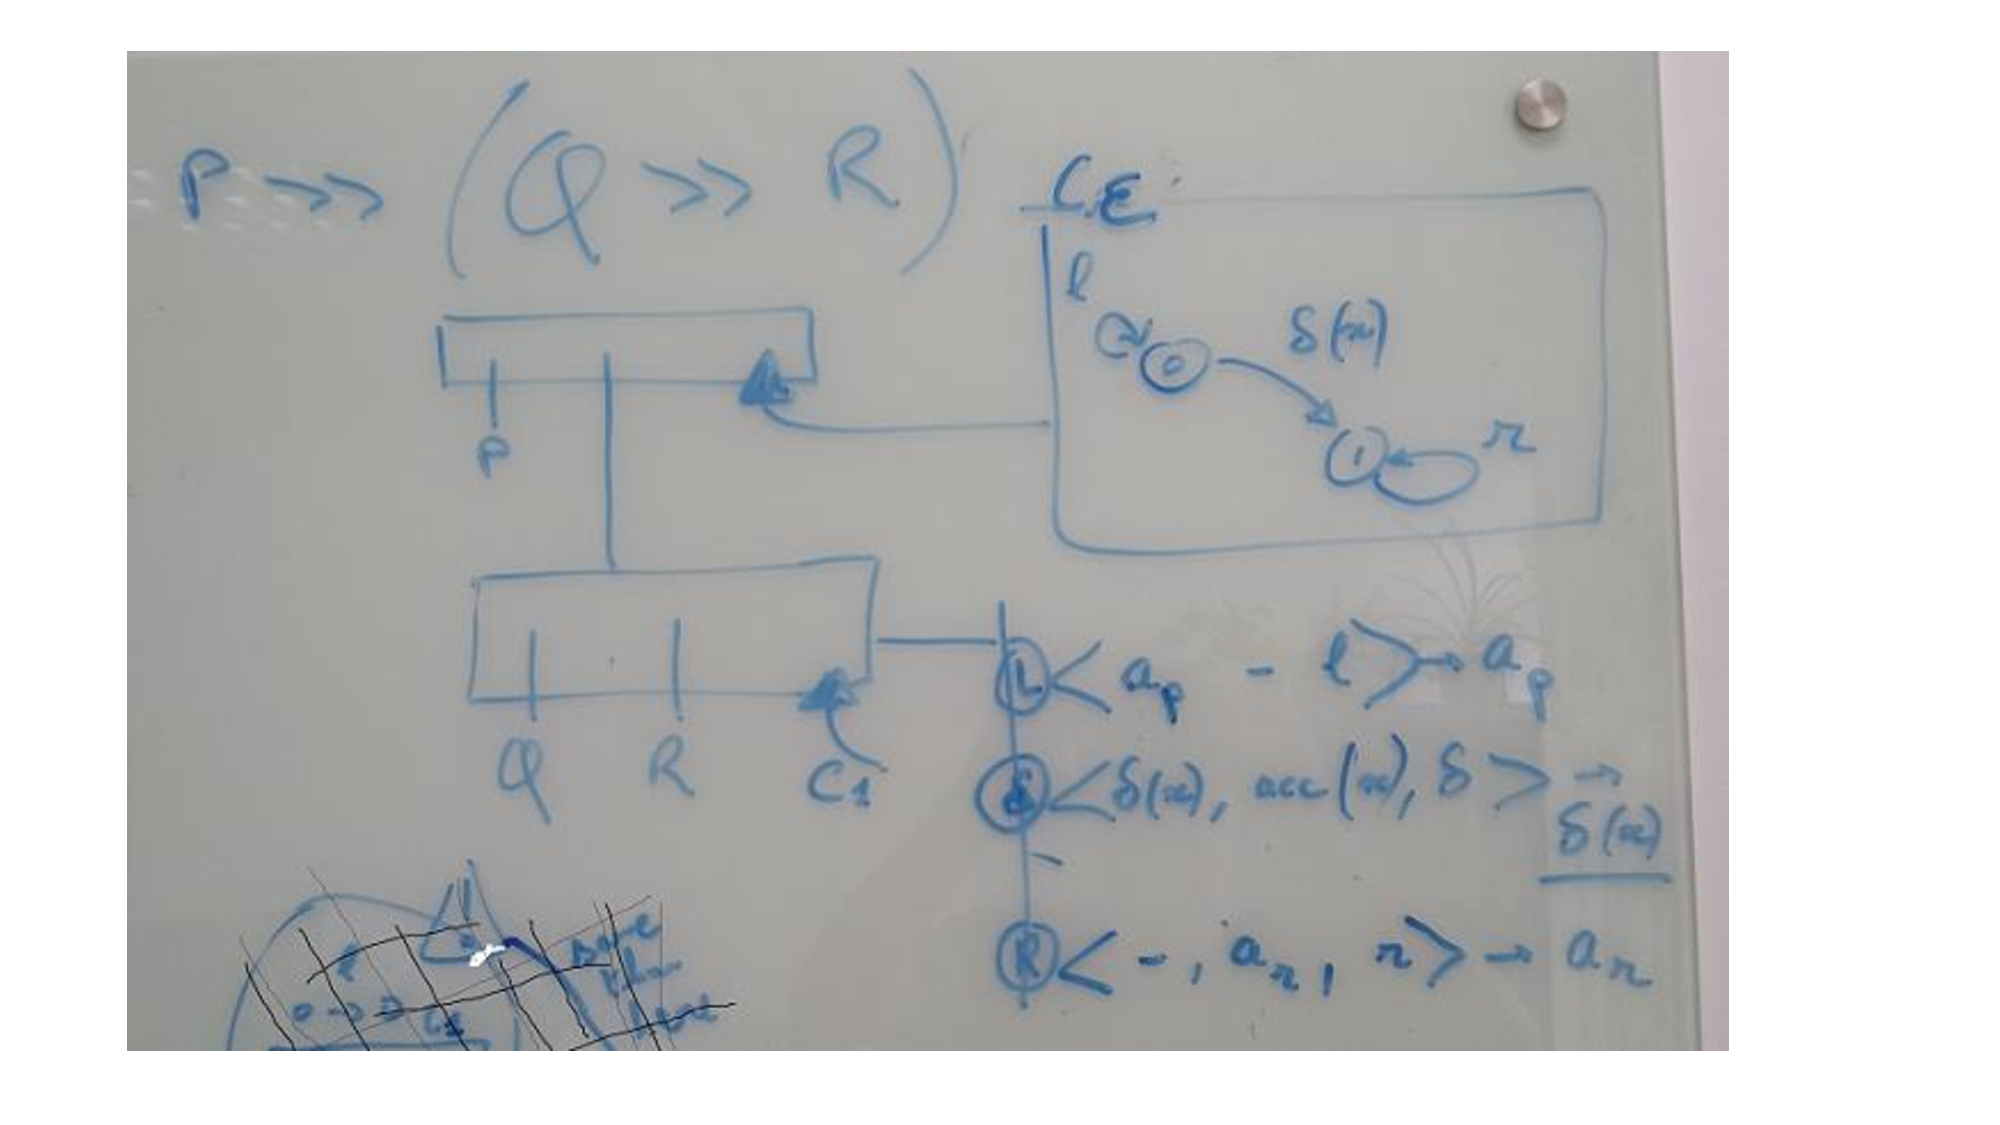
\includegraphics[width=0.5\linewidth]{XFIG/Struct-P-QR}
% 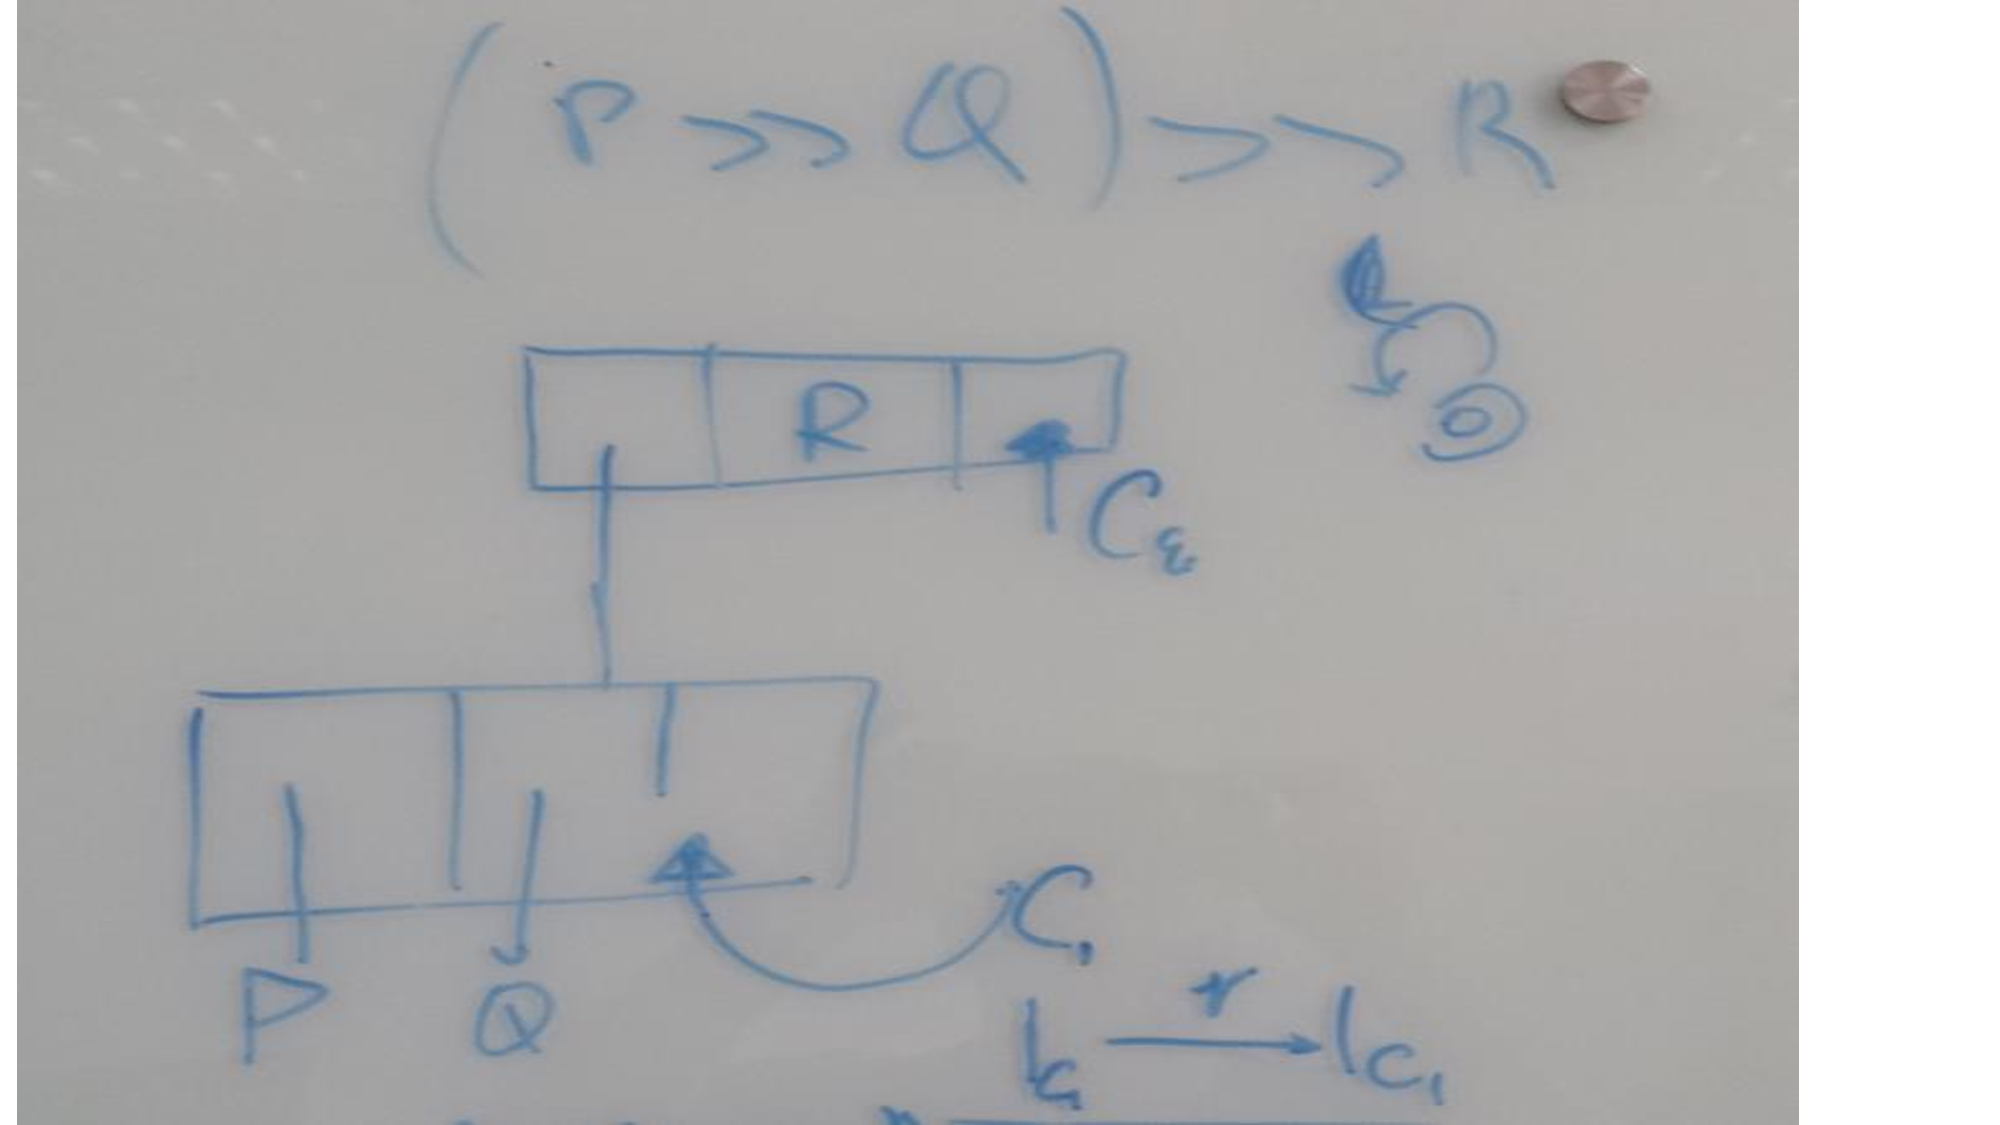
\includegraphics[width=0.35\linewidth]{XFIG/Struct-PQ-R}}
  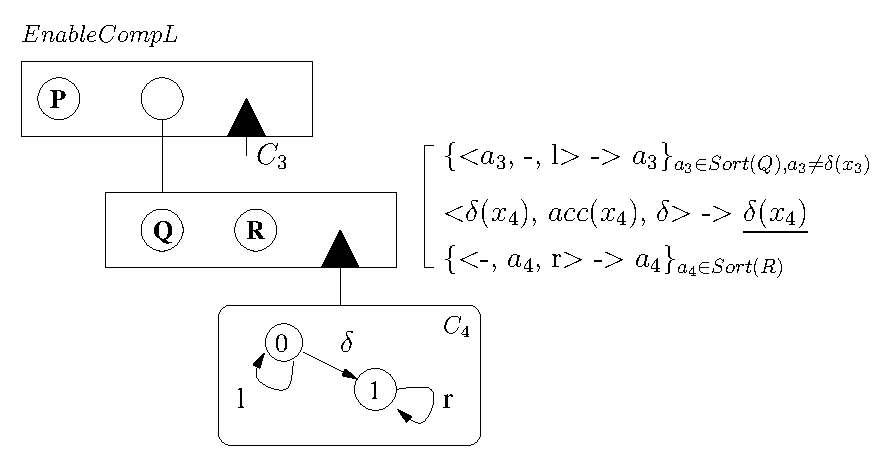
\includegraphics[width=0.60\linewidth]{XFIG/P-QR}
  \hspace{5mm}
 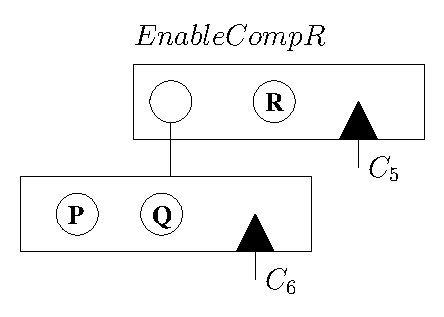
\includegraphics[width=0.27\linewidth]{XFIG/PQ-R}}
  \caption{Structure of the pNets for ``P>>(Q>>R) and (P>>Q)>>R''}
  \label{schema:enable-assoc}
\end{figure}

The two open pNets are drawn in Fig. \ref{schema:enable-assoc}. To
alleviate the drawing, we have only 
  given one instance (C2) of the enable controller pLTSs, and one example of
  the set of synchronisation vectors.

  Below we give the two open automata for these pNets. In the
  open-transitions in these 
    automata, the predicates are very simple, and for readability
    we show them directly in the transitions.
    Remark that while the structure of the automaton states is useful
    for their construction, it is not relevant later, so we have
    dropped this structure when drawing the automaton.

\begin{figure}[h]
  \begin{minipage}{2cm}
  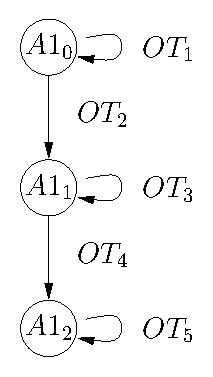
\includegraphics[width=\linewidth]{XFIG/PQR-automaton}
  \end{minipage}
  \hspace{10mm}
  \begin{minipage}{7cm}
  \begin{eqnarray*}
    OT_1 & = \openrule{0 \xrightarrow{l}_{C_3} 0
    	\\\xrightarrow{a1}_P\\ a1\neq\delta(x)}
    {\ostate{00} \OTarrow{a1} \ostate{00}}\\
    OT_2 & = \openrule{
                       0 \xrightarrow{\delta}_{C_3} 1, ~~
                            0 \xrightarrow{l}_{C_4} 0,  ~~                 
                            \{\xrightarrow{\delta(x1)}_P, ~~
                            \xrightarrow{acc(x1)}_Q\}
                      }
                      {\ostate{00} \OTarrow{\underline{\delta(x1)}} \ostate{10}}    \\
    OT_3 & = \openrule{0 \xrightarrow{l}_{C_4} 0,
                        \\1 \xrightarrow{r}_{C_3} 1,\\
                        \xrightarrow{a2}_Q,\\a2\neq\delta(x)
                        }
    {\ostate{10} \OTarrow{a2} \ostate{10}}\\
    OT_4 & = \openrule{
                       0 \xrightarrow{\delta}_{C_4} 1, \qquad
                       1 \xrightarrow{r}_{C_3} 1, \qquad
                       \{\xrightarrow{\delta(x2)}_Q, \qquad 
                       \xrightarrow{acc(x2)}_R\} 
                       }
                      {\ostate{10} \OTarrow{\underline{\delta(x2)}} \ostate{11}}    \\
    OT_5 & = \openrule{1 \xrightarrow{r}_{C_3} 1, \\1 \xrightarrow{r}_{C_4} 1, 
    	\\\xrightarrow{a3}_R
    	}
    {\ostate{11} \OTarrow{a3} \ostate{11}}
    \end{eqnarray*}
  \end{minipage}
  \caption{Open Automaton for the term ``P>>(Q>>R)''}
  \label{schema:enable3bis}
\end{figure}

\begin{figure}[t]
  \begin{minipage}{2cm}
  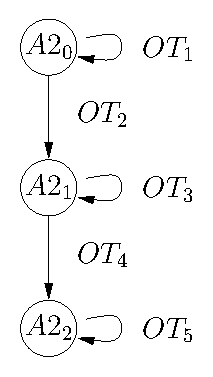
\includegraphics[width=\linewidth]{XFIG/PQR2-automaton}
  \end{minipage}
  \hspace{10mm}
  \begin{minipage}{7cm}
  \begin{eqnarray*}
    OT'_1 & = \openrule
             {
               0 \xrightarrow{l}_{C_3} 0,~~0 \xrightarrow{l}_{C_4} 0,~~
               \{\xrightarrow{b1}_P\},~~ b1\neq\delta(y)
               }
             {\ostate{00} \OTarrow{b1} \ostate{00}}\\
    OT'_2 & = \openrule
             {
                       0 \xrightarrow{l}_{C_5} 0, ~~
                       0 \xrightarrow{\delta}_{C_6} 1,  ~~
              \{\xrightarrow{\delta(y1)}_P,~~      \xrightarrow{acc(y1)}_Q\}~~ 
                      }
             {\ostate{00} \OTarrow{\underline{\delta(y1)}} \ostate{01}}\\
    OT'_3 & = \openrule
             {
               0 \xrightarrow{l}_{C_5} 0,\\0 \xrightarrow{r}_{C_6} 0,
               \\ \{\xrightarrow{b2}_Q\},\\b2\neq\delta(y)
               }
    {\ostate{01} \OTarrow{b2} \ostate{01}}\\
    OT'_4 & = \openrule
             {
                       0 \xrightarrow{\delta}_{C_5} 1, ~~
                       1 \xrightarrow{r}_{C_6} 1, ~~\{\xrightarrow{\delta(y2)}_Q, ~~
                    \xrightarrow{accept(y2)}_R\} 
                                 }
             {\ostate{01} \OTarrow{\underline{\delta(y2)}} \ostate{11}}    \\
    OT'_5 & = \openrule
             {1 \xrightarrow{r}_{C_5} 1,\\\{\xrightarrow{b3}_R\}
             	}
             {\ostate{11} \OTarrow{b3} \ostate{11}}
    \end{eqnarray*}
  \end{minipage}
%  \label{schema:enable5}
\end{figure}

In this example, we have no state variables in the pNets leaves, so we
need no auxiliary predicate in the FH-bisimulation.

Let us build a relation
    $R = \{(A1_0,A2_0), (A1_1,A2_1), (A1_2,A2_2)\}$, and prove that
    $R$ is a strong FH-bisimulation.

    Pick e.g. transition $OT_1$ of automaton $A1$, we have
    $A1_0 \xrightarrow{OT_1}_{A1} A1_0$. The matching transition from
    $A2_0$ is $OT'_1$, with 
    $A2_0 \xrightarrow{OT'_1}_{A2} A2_0$, the set of holes involved in
    both transitions is $\{P\}$, and the resulting state is in the
    bisimulation ($A1_0 ~ A2_0$).
    The proof obligation is:
    
    $$  a1\neq\delta(x) \implies
         a1=b1 \implies b1\neq\delta(y) \land a1=b1 $$

    The proof obligation for $OT_2$ versus $OT'_2$ is still simpler:

    $$ \delta(x_1)=\delta(y_1) \land acc(x_1)=acc(y_1)
       \implies \underline{\delta(x_1)}=\underline{\delta(y_1)} $$

       the 3 other cases, and the 5 in the other direction, are left
       to the reader. All are simple to prove, so $R$ is a
       FH-bisimulation, and the initial states of the 2 pNets are equivalent.
           \qed
       
       This proof shows how the flattening induced by the open transitions makes the 
       reasoning on hierarchical structures easy, while keeping a structured view of the 
       compared systems.

       
       \newpage
       
       \section{Proofs of basic properties on pNets}
       \subsection{Equivalence relation (Theorem~\ref{thm-equiv})}
        \emph{Suppose $\mathcal{R}$ 
       	is an FH-bisimulation. Then $\mathcal{R}$ is an equivalence, that is, 
       	$\mathcal{R}$ is 
       	reflexive, symmetric and transitive.
       	}
%%% A PROOF WITH CONSTRUCTIVE AERGUMENTS BUT THAT DOES NOT WORK
       
%       \begin{proof}
%
%       It is trivial to check reflexivity and symmetry. Here we focus on the
%transitivity. 
%To prove transitivity of strong FH-bisimulation on pNets it is sufficient to prove 
%transitivity of the strong FH-bisimulation on states of their Open Automata. Consider 3 
%open automata 
%$\mathcal{T}_1$, $\mathcal{T}_2$, $\mathcal{T}_3$ and states $s^1$, $s^2$, $s^3$ in 
%those 
%automata\footnote{We omit the constraints stating that each $s^i_x$ is in the states of 
%$\mathcal{T}_i$ for the sake of readability}.
%Suppose we have $\mathcal{R}$ an FH-bisimulation relation between states of 
%$\mathcal{T}_1$ and of  $\mathcal{T}_2$; members of $\mathcal{R}$ are of the form 
%$(s^1,s^2|\Pred)$.
%Suppose we also  have $\mathcal{R}'$ an FH-bisimulation relation between states of 
%$\mathcal{T}_2$ and of  $\mathcal{T}_3$; members of $\mathcal{R}2$ are of the form 
%$(s^2,s^3|\Pred\,')$.
%We use $\fv$ a function returning the free variables of a term/automaton.
%
%Let $\mathcal{R}''$ be the relation (We denote $\Phi$ a set of renamings): 
%
%%\begin{mathpar}
%%\inferrule{}
%%{}
%%\end{mathpar}
%
%\[\mathcal{R}'' = \Big\{(s^1,s^3|\Pred\,'')\Big|
%\displaystyle
% \begin{array}[t]{l}\exists (s^2_p)^{p\in P}.\,\exists (\Phi_p)^{p\in P}.\,\\
%\quad 
%	\big(\begin{array}{l}
%	\forall p\in P.\, (s^1,s^2_p|\Pred)\in\mathcal{R}\land 
%	(s^2_p,s^3|\Pred\,')\in\mathcal{R}'\land \\
%	 \forall\ \phi\in\Phi_p.\,
%	  \fv((\Pred\land\Pred')\phi)\subseteq \fv(\mathcal{T}_1)\cup\fv(\mathcal{T}_3) \land
%	  \dom(\phi)\subseteq \fv(\mathcal{T}_2)
%	\end{array}
%	\big)\\
%\quad
%\land ~\Pred'' =\displaystyle\bigvee_{\begin{array}{l}
%	p\in P\\\phi\in \Phi_p
%	\end{array}} (\Pred\land\Pred\,')\phi
%	
%\end{array}\Big\}
%\]
%%(s^1,s^2|\Pred)\in\mathcal{R}\\ (s^2,s^3|\Pred\,')\in\mathcal{R}' 	
%%}\!\!\!\!\!\exists \phi.\begin{array}[t]{l} \\
%%\land 
%%\\
%%\land 
%%\\
%\TODO{s2p is the family of states that relate s1 and s2 big phi is the set of renamings 
%for each s2 in the family}
%
%The relation is built as follows: for each pair of state $s^1$, $s^3$, for each state 
%$s^2$ such that $\mathcal{R}$ relates $s^1$ and $s^2$, and $\mathcal{R}'$ relates $s^2$ 
%and $s^3$, we take the conjunction of the two predicates. The predicates for different 
%values of $s^2$ are collected by a disjunction. 
%Finally, a set of substitutions should ensure that the 
%free variables of the predicates are only the ones of $\mathcal{T}_1$ and 
%$\mathcal{T}_1$. These substitutions somehow express the different ways to match the two 
%predicates by eliminating the 
%free variables. We simplify the proof to the case where a single substitution is 
%necessary for each state $s^2$; the extension to a set of substitution is relatively 
%simple but complicates the notations. $\phi_p$ is this set of substitutions in the proof 
%below.
%
% We will show
%that $\mathcal{R}''$ is an FH-bisimulation. Consider 
%$(s^1,s^3|\Pred\,'')\in\mathcal{R}''$. Then there is a set of states of 
%$\mathcal{T}_2$ relating $s^1$ and $s^3$, let $(s^2_p)^{p\in P}$ be this family.  
%For any $p\in P$ by definition of $\mathcal{R}''$,
%$(s^1,s^2_p|\Pred_p)\in\mathcal{R}$,  and $(s^2_p,s^3|\Pred\,'_p)\in\mathcal{R}$. 
%Additionally we have $\Pred\,'' = \bigvee_{p\in P} (\Pred_p\land\Pred_p)\,'\phi_p$.
%We have 
%the 
%following by definition of bisimulation.
%For any open transition $OT$ in $\mathcal{T}_1$ originating from $s^1$:
%
%\begin{mathpar}
%
%\inferrule*[myfraction=\reddottedrule]
%{\{s^1_i\xrightarrow{a_i}_i {s^{1}}'_i\}^{i\in I_1}, % , s^1_i,s^{1'}_i\in
%	%States(I_1)
%	\{\xrightarrow{b_j}_j\}^{j\in J_1},\Pred_{OT},\Post_{OT}}
%{s^1 \xrightarrow {v} {s^{1}}'}
%
%\end{mathpar}
%
%there exist open transitions $OT_{p x}^{x\in X} \subseteq \mathcal{T}_2$:
%
%\begin{mathpar}
%
%%    \left( fresh \ \overline{a_i}, \overline{b_j}, v_x.\ \
%\inferrule*[myfraction=\reddottedrule]
%{\{s^{2}_{pi}\xrightarrow{a_{p i x}}_i s^{2}_{p i x}\}^{i\in I_{2 p x}},
%	\{\xrightarrow{b_{j p x}}_j\}^{j\in J_{2px}}, \Pred_{OT_{px}},\Post_{OT_{px}}}
%{s^2_p \xrightarrow {v_{px}} s^{2}_{px}}
%%         \right)
%\end{mathpar}
%
%such that  $\forall x, J_1=J_{2px}, (s^{1'},s^{2}_{px}|\Pred_{target_{px}})\in 
%\mathcal{R}$;
%and  \\
%
%$\Pred_p \land \Pred_{OT}\\
%\hspace{1cm} \implies\!\!\! \bigvee_{x\in X}
%\left( \forall j. b_j=b_{jpx}  \Rightarrow \Pred_{OT_{px}}
%\land v\!=\!v_{px} \land
%\Pred_{target_{px}}\subst{\Post_{OT}}\subst{\Post_{OT_{px}}}\right)$
%
%for any open transition $OT_{px}$, since
%$(s^2_p,s^3|\Pred\,^\prime_p)\in\mathcal{R}'$ there exist open transitions
%$OT_{pxy}^{x\in X, y\in Y} \subseteq \mathcal{T}_3$: 
%
%\begin{mathpar}
%
%%    \left( fresh \ \overline{a_i}, \overline{b_j}, v_x.\ \
%\inferrule*[myfraction=\reddottedrule]
%{\{s^{3}_i\xrightarrow{a_{i p x y}}_i s^{3}_{i p x y}\}^{i\in I_{3 p x y}},
%	\{\xrightarrow{b_{j p x y}}_j\}^{j\in J_{3pxy}}, \Pred_{OT_{pxy}},\Post_{OT_{pxy}}}
%{s^3 \xrightarrow {v_{pxy}} s^{3}_{pxy}}
%%         \right)
%
%\end{mathpar}
%such that  $\forall y, J_{2px}=J_{3pxy}, 
%(s^{2}_x,s^{3}_{pxy}|\Pred_{target_{pxy}})\in \mathcal{R}'$; and  \\
%$\Pred\,'_p \land \Pred_{OT_{px}}\\
%\hspace{1cm} \implies\!\!\! \bigvee_{y\in Y}
%\left( \forall j. b_{jpx}=b_{jpxy}  \Rightarrow \Pred_{OT_{pxy}}
%\land v_{px}\!=\!v_{pxy} \land
%\Pred_{target_{pxy}}\subst{\Post_{OT_{px}}}\subst{\Post_{OT_{pxy}}}\right)$.
%
%This is verified for each $p\in P$. Overall,  we have a family of open transitions 
%$OT_{pxy}^{p\in 
%P, x\in X, 
%y\in Y} \subseteq \mathcal{T}_3$ that should simulate \emph{OT}.
%
%First, $\forall y, \forall x, \forall p, J_1=J_{2px}=J_{3pxy}, 
%({s^{1}}',s^{3}_{pxy}|\Pred\,'_{target_{pxy}})\in \mathcal{R}''$. 
%Indeed for any 
%$p$, 
%$x$, and 
%$y$, $s^2_{px}$
%relate ${s^{1}}'$ and $s^{3}_{pxy}$, indeed
%$(s^{1'},s^{2}_{px}|\Pred_{target_{px}})\in \mathcal{R}$
% and $(s^{2}_x,s^{3}_{pxy}|\Pred_{target_{pxy}})\in \mathcal{R}'$. 
% More precisely, $s^{2}_{px} \in ({s^{2}_p}')^{p\in P'}$ where $({s^{2}_p}')^{p\in 
% P'}$ 
% is 
% the set of states relating ${s^{1}}'$ and $s^{3}_{pxy}$.
%Consequently, for all $p$, $x$, $y$,\\
% $\left(\exists \phi'.\,(\Pred_{target_{px}}\land 
%\Pred_{target_{pxy}})\phi'\land \fv((\Pred\land\Pred)\phi')\subseteq 
%\fv(\mathcal{T}_1)\cup\fv(\mathcal{T}_3)\right)\implies 
%\Pred\,'_{target_{pxy}}$ \\
%This is one element of the  disjunction defining the 
%predicate 
%relating ${s^{1}}'$ and $s^{3}_{pxy}$ in the definition of $\mathcal{R}''$.
%
%Second, we need \\
%\begin{small}
%$\Pred\,'' \land \Pred_{OT}\\
%\hspace{1cm} \implies\!\!\! \bigvee_{x\in X}\bigvee_{y\in Y}\bigvee_{p\in P}
%\left( \forall j. b_j=b_{jpxy}  \Rightarrow \Pred_{OT_{pxy}}
%\land v\!=\!v_{pxy} \land
%\Pred\,'_{target_{pxy}}\subst{\Post_{OT}}\subst{\Post_{OT_{pxy}}}\right)$.
%\end{small}
%
%We have, for all $p$
%\begin{small}
%$\Pred_p \land \Pred_{OT}\land\Pred'_p\\
%\hspace{1cm} \implies\!\!\! \bigvee_{x\in X}
%\left( \forall j. b_j=b_{jpx}  \Rightarrow \Pred_{OT_{px}}
%\land v\!=\!v_{px} \land
%\Pred_{target_{px}}\subst{\Post_{OT}}\subst{\Post_{OT_{px}}}\right)\land\Pred'_p\\
%%
%\hspace{1cm} \implies\!\!\! \bigvee_{x\in X}
%\left( \forall j. b_j=b_{jpx}  \Rightarrow (\Pred_{OT_{px}}\land\Pred'_p)
%\land v\!=\!v_{px} \land
%\Pred_{target_{px}}\subst{\Post_{OT}}\subst{\Post_{OT_{px}}}\right)\\
%%
%\hspace{1cm} \implies\!\!\! \bigvee_{x\in X}
%\big( \forall j. b_j=b_{jpx}  \Rightarrow (\bigvee_{y\in Y} 
%\big( \forall j'. b_{j'px}=b_{j'pxy}  \Rightarrow \Pred_{OT_{pxy}}
%\land v_{px}\!=\!v_{pxy}\\\hspace{3em}~ \land
%\Pred_{target_{pxy}}\subst{\Post_{OT_{px}}}\subst{\Post_{OT_{pxy}}}\big))
%\land v\!=\!v_{px} \land
%\Pred_{target_{px}}\subst{\Post_{OT}}\subst{\Post_{OT_{px}}}\big)\\
%%
%\hspace{1cm} \implies\!\!\! \bigvee_{x\in X} \bigvee_{y\in Y}
%\big( \forall j, j'. b_j=b_{jpx} \land b_{j'px}=b_{j'pxy}
%\Rightarrow \big( 
%\Pred_{OT_{pxy}}
%\land v\!=v_{px}\!=\!v_{pxy}\\\hspace{3em}~ \land
%\Pred_{target_{pxy}}\subst{\Post_{OT_{px}}}\subst{\Post_{OT_{pxy}}}
% \land
%\Pred_{target_{px}}\subst{\Post_{OT}}\subst{\Post_{OT_{px}}}\big)\big)
%$
%
%\end{small}
%
%Additionally, the Post substitutions only have an effect on the  predicates that  use 
%some of the 
%substituted 
%variables, and because of the domain of the substitutions we have:\\
%$(\Pred_{target_{px}}\subst{\Post_{OT}}\subst{\Post_{OT_{px}}}\land 
%\Pred_{target_{pxy}}\subst{\Post_{OT_{px}}}\subst{\Post_{OT_{pxy}}})\phi\\
%%
%= 
%(\Pred_{target_{px}}\subst{\Post_{OT}}\subst{\Post_{OT_{px}}}\subst{\Post_{OT_{pxy}}}\land
%\Pred_{target_{pxy}}\subst{\Post_{OT}}\subst{\Post_{OT_{px}}}\subst{\Post_{OT_{pxy}}}) 
%\phi\\
%%
%= 
%((\Pred_{target_{px}}\land
%\Pred_{target_{pxy}})\subst{\Post_{OT_{px}}}\phi) 
%\subst{\Post_{OT}}\subst{\Post_{OT_{pxy}}}\\
%%
%\implies\Pred\,'_{target_{pxy}}\subst{\Post_{OT}}
%\subst{\Post_{OT_{pxy}}}\\
% $
%Finally, gathering the previous results, and using the fact that only variables of 
%$\mathcal{T}_2$ are changed by $\phi$ substitutions:
%
%$\Pred\,'' \land \Pred_{OT}\\
%\hspace{1cm} \implies\!\!\! \bigvee_{p\in P}(\Pred_p \land 
%\Pred_{OT}\land\Pred\,'_p)\phi\\
%\hspace{1cm} \implies\!\!\! \bigvee_{x\in X}\bigvee_{y\in Y}\bigvee_{p\in P}
%\left( \forall j. b_j=b_{jpxy}  \Rightarrow \Pred_{OT_{pxy}}
%\land v\!=\!v_{pxy} \land
%\Pred\,'_{target_{pxy}}\subst{\Post_{OT}}\subst{\Post_{OT_{pxy}}}\right)
%$
%
%This is the expected property.
%
%
%\smallskip
%Concerning the other direction of bisimulation, it is sufficient to notice that the role 
%of $s^1$ and $s^3$ in the definition of $\mathcal{R}''$ is symmetrical, and thus the 
%proof is similar.
%
%       \end{proof}
%       
%       \bigskip
%       
%       
              \begin{proof}
       	
       	It is trivial to check reflexivity and symmetry. Here we focus on the
       	transitivity. 
       	To prove transitivity of strong FH-bisimulation on pNets it is sufficient to 
       	prove 
       	transitivity of the strong FH-bisimulation on states. Consider 3 open automata 
       	$\mathcal{T}_1$, $\mathcal{T}_2$, $\mathcal{T}_3$ and states $s$, $t$, $u$ 
       	in those 
       	automata\footnote{We omit the constraints stating that each $s_x,\,t_x,\,u_x$ is 
       	in the 
       	states of 
       		$\mathcal{T}_1,\,\mathcal{T}_2,\,\mathcal{T}_3$ for the sake of readability}.
       	Suppose we have $\mathcal{R}$ an FH-bisimulation relation between states of 
       	$\mathcal{T}_1$ and of  $\mathcal{T}_2$; members of $\mathcal{R}$ are of the form 
       	$(s,t|\Pred_{s,t})$.
       	Suppose we also  have $\mathcal{R}'$ an FH-bisimulation relation between states 
       	of 
       	$\mathcal{T}_2$ and of  $\mathcal{T}_3$; members of $\mathcal{R}'$ are of the 
       	form 
       	$(t,u|\Pred_{t,u})$.
       	
       	Let $\mathcal{R}''$ be the relation: 
       	\[\mathcal{R}'' = 
       	\{(s,u|\Pred_{s,u})\,\,\Big|\,\Pred_{s,u}=\bigvee_{\begin{array}{c}       		
       		(s,t|\Pred_{s,t})\in\mathcal{R}\\ (t,u|\Pred_{t,u})\in\mathcal{R}' 	
       		\end{array}
       	}\,\Pred_{s,t}\land\Pred_{t,u}\}\]

This relation is the adaptation of the transitivity to the conditional relationship that 
defines a bisimulation. Indeed the global disjunction together with the conjunction of 
predicates plays exactly the role of the intermediate element in a transitivity rule: 
``there exists an intermediate state'' corresponds to the global disjunction, and the 
conjunction of states expresses the intermediate predicate is used to ensure 
satisfiability of the predicate relating the first state to the last one.
       	
       	The relation is built as follows: for each pair of states $s$, $u$, for each 
       	state 
       	$t$ such that $\mathcal{R}$ relates $s$ and $t$, and $\mathcal{R}'$ relates 
       	$t$ 
       	and $u$, we take the conjunction of the two predicates. The predicates for 
       	different 
       	values of $t$ are collected by a disjunction. 
       	
       	We will show
       	that $\mathcal{R}''$ is an FH-bisimulation. Consider 
       	$(s,u|\Pred_{s,u})\in\mathcal{R}''$. Then there is a set of states of 
       	$\mathcal{T}_2$ relating $s$ and $u$, let $(t_p)^{p\in P}$ be this family.  
       	       	We have $\Pred_{s,u} = \bigvee_{p\in P} \Pred_{s,p}\land\Pred_{p,u}$.

\medskip

       	For any $p\in P$ by definition of $\mathcal{R}''$,
       	$(s,t_p|\Pred_{s,p})\in\mathcal{R}$,  and 
       	$(t_p,u|\Pred\,'_{p,u})\in\mathcal{R}'$. 
       	We have 
       	the 
       	following by definition of bisimulation:
       	For any open transition $OT$ in $\mathcal{T}_1$ originating from $s$.
       	\begin{mathpar}
       	
       	\inferrule*[myfraction=\reddottedrule]
       	{\{s_i\xrightarrow{a_i}_i {s}'_i\}^{i\in I_1}, % , s^1_i,s^{1'}_i\in
       		%States(I_1)
       		\{\xrightarrow{b_j}_j\}^{j\in J_1},\Pred_{OT},\Post_{OT}}
       	{s \OTarrow {v} {s}'}
       	
       	\end{mathpar}
       	
       	There exist open transitions $OT_{p x}^{x\in X} \subseteq \mathcal{T}_2$:
       	
       	\begin{mathpar}
       	
       	%    \left( fresh \ \overline{a_i}, \overline{b_j}, v_x.\ \
       	\inferrule*[myfraction=\reddottedrule]
       	{\{t_{p i}\xrightarrow{a_{p i x}}_i t_{p i x}\}^{i\in I_{p x}},
       		\{\xrightarrow{b_{j p x}}_j\}^{j\in J_{px}}, \Pred_{OT_{px}},\Post_{OT_{px}}}
       	{t_p \OTarrow {v_{px}} t_{p x}}
       	%         \right)
       	\end{mathpar}
       	
       	such that  $\forall x, J_1=J_{px}, (s',t_{px}|\Pred_{{px}})\in 
       	\mathcal{R}$;
       	and  \\
       	
       	$\Pred_{s,p} \land \Pred_{OT}\\
       	\hspace{1cm} \implies\!\!\! \bigvee_{x\in X}
       	\left( \forall j. b_j=b_{jpx}  \Rightarrow \Pred_{OT_{px}}
       	\land v\!=\!v_{px} \land
       	\Pred_{{px}}\subst{\Post_{OT}}\subst{\Post_{OT_{px}}}\right)$\\
       	


For any open transition $OT_{px}$, since
       	$(t_p,u|\Pred_{p,u})\in\mathcal{R}'$ there exist open transitions
       	$OT_{pxy}^{y\in Y} \subseteq \mathcal{T}_3$: 
       	
       	\begin{mathpar}
       	
       	%    \left( fresh \ \overline{a_i}, \overline{b_j}, v_x.\ \
       	\inferrule*[myfraction=\reddottedrule]
       	{\{u_i\xrightarrow{a_{i p x y}}_i u_{i p x y}\}^{i\in I_{p x y}},
       		\{\xrightarrow{b_{j p x y}}_j\}^{j\in J_{pxy}}, 
       		\Pred_{OT_{pxy}},\Post_{OT_{pxy}}}
       	{u \OTarrow {v_{pxy}} u_{pxy}}
       	%         \right)
       	
       	\end{mathpar}
       	such that  $\forall y, J_{px}=J_{pxy}, 
       	(t_{px},u_{pxy}|\Pred_{{pxy}})\in \mathcal{R}'$; and  \\
       	$\Pred\,'_{p,u} \land \Pred_{OT_{p x}}\\
       	\hspace{1cm} \implies\!\!\! \bigvee_{y\in Y}
       	\left( \forall j. b_{jpx}=b_{jpxy}  \Rightarrow \Pred_{OT_{pxy}}
       	\land v_{px}\!=\!v_{pxy} \land
       	\Pred_{{pxy}}\subst{\Post_{OT_{px}}}\subst{\Post_{OT_{pxy}}}\right)$\\.
       	
       	This is verified for each $p\in P$. Overall,  we have a family of open 
       	transitions 
       	$OT_{pxy}^{p\in 
       		P, x\in X, 
       		y\in Y} \subseteq \mathcal{T}_3$ that should simulate \emph{OT}.

       	
       	
       	First,  $\forall y, \forall x, \forall p, J_1=J_{px}=J_{pxy}, 
       	({s}',u_{pxy}|\Pred\,'_{{pxy}})\in \mathcal{R}''$. 
       	Indeed for any 
       	$p$, 
       	$x$, and 
       	$y$, $t_{px}$
       	relate ${s}'$ and $u_{pxy}$, indeed
       	$(s',t_{px}|\Pred_{{px}})\in \mathcal{R}$
       	and $(t_{px},u_{pxy}|\Pred_{{pxy}})\in \mathcal{R}'$. 
       	More precisely, $t_{px} \in ({t'_p})^{p\in P'}$ where $({t'_p})^{p\in 
       		P'}$ is 
       	the set of states relating ${s}'$ and $u_{pxy}$.
       	Consequently, for all $p$, $x$, $y$, $\Pred_{px}\land 
       	\Pred_{{pxy}}\implies 
       	\Pred\,'_{{pxy}}$ (this is one element of the  disjunction defining the 
       	predicate 
       	relating ${s}'$ and $u_{pxy}$ in the definition of $\mathcal{R}''$).


One can notice that, as bisimulation predicates are used to relate states that 
belong to two different open automata, the free variables of these predicates 
that do not belong to the two related automata can safely be renamed to avoid any 
name clash. In practice,
we can suppose that, as $\Pred\,'_{{pxy}}$ is used to relate states of 
$\mathcal{T}_1$, and $\mathcal{T}_3$, there exists a predicate obtained by 
renaming variables, that is equivalent to $\Pred\,'_{{pxy}}$ and does not 
contain the variables of 	$\mathcal{T}_2$. This predicate with ``fresh'' 
variables is called   $\Pred\,'_{{pxy}}$ in the following.
Similarly, we can suppose that $\Pred_{{px}}$ contains no 
variable in $\mathcal{T}_3$, and $\Pred_{{pxy}}$ contains no 
variable in $\mathcal{T}_1$.
       	
       	Second, by definition of bisimulation we need (recall that $\Pred_{s,u}$ is the 
       	original predicate relating $s$ and $u$ by definition of the transitive 
       	closure):\\
       	\begin{small}
       		$\Pred_{s,u} \land \Pred_{OT}\\
       		\hspace{1cm} \implies\!\!\! \bigvee_{x\in X}\bigvee_{y\in Y}\bigvee_{p\in P}
       		\left( \forall j. b_j=b_{jpxy}  \Rightarrow \Pred_{OT_{pxy}}
       		\land v\!=\!v_{pxy} \land
       		\Pred\,'_{{pxy}}\subst{\Post_{OT}}\subst{\Post_{OT_{pxy}}}\right)$.
       	\end{small}
\TODO{From we will add notation (1) and (2)}        	
       	We have, for all $p$
       	\begin{small}
       		$\Pred_{s,p} \land \Pred_{OT}\land\Pred_{p,u}\\
       		\hspace{1cm} \implies\!\!\! \bigvee_{x\in X}
       		\left( \forall j. b_j=b_{jpx}  \Rightarrow \Pred_{OT_{px}}
       		\land v\!=\!v_{px} \land
       		\Pred_{{px}}\subst{\Post_{OT}}\subst{\Post_{OT_{px}}}\right)\land\Pred_{p,u}\\
       		%
       		\hspace{1cm} \implies\!\!\! \bigvee_{x\in X}
       		\left( \forall j. b_j=b_{jpx}  \Rightarrow (\Pred_{OT_{px}}\land\Pred_{p,u})
       		\land v\!=\!v_{px} \land
       		\Pred_{{px}}\subst{\Post_{OT}}\subst{\Post_{OT_{px}}}\right)\\
       		%
       		\hspace{1cm} \implies\!\!\! \bigvee_{x\in X}
       		\big( \forall j. b_j=b_{jpx}  \Rightarrow (\bigvee_{y\in Y} 
       		\big( \forall j'. b_{j'px}=b_{j'pxy}  \Rightarrow \Pred_{OT_{pxy}}
       		\land v_{px}\!=\!v_{pxy}\\\hspace{3em}~ \land
       		\Pred_{{pxy}}\subst{\Post_{OT_{px}}}\subst{\Post_{OT_{pxy}}}\big))
       		\land v\!=\!v_{px} \land
       		\Pred_{{px}}\subst{\Post_{OT}}\subst{\Post_{OT_{px}}}\big)\\
       		%
       		\hspace{1cm} \implies\!\!\! \bigvee_{x\in X} \bigvee_{y\in Y}
       		\big( \forall j, j'. b_j=b_{jpx} \land b_{j'px}=b_{j'pxy}
       		\Rightarrow \big( 
       		\Pred_{OT_{pxy}}
       		\land v\!=v_{px}\!=\!v_{pxy}\\\hspace{3em}~ \land
       		\Pred_{{pxy}}\subst{\Post_{OT_{px}}}\subst{\Post_{OT_{pxy}}}
       		\land
       		\Pred_{{px}}\subst{\Post_{OT}}\subst{\Post_{OT_{px}}}\big)\big)
       		$
       		
       	\end{small}
       	
By construction, four substitutions $\subst{~}$ only have an effect on the  
variables of the open automaton they belong to, they also produce terms containing only 
variables of the open automaton they belong to. Finally, because of the domain of the 
substitutions  and of the predicates, we have:\\
       	$\Pred_{{px}}\subst{\Post_{OT}}\subst{\Post_{OT_{px}}}\land 
       	\Pred_{{pxy}}\subst{\Post_{OT_{px}}}\subst{\Post_{OT_{pxy}}}\\
       	\Leftrightarrow % we changed =
       	\Pred_{{px}}\subst{\Post_{OT}}\subst{\Post_{OT_{px}}}\subst{\Post_{OT_{pxy}}}\land
       	\Pred_{{pxy}}\subst{\Post_{OT}}\subst{\Post_{OT_{px}}}\subst{\Post_{OT_{pxy}}}\\
       	\implies\Pred\,'_{{pxy}}\subst{\Post_{OT}}\subst{\Post_{OT_{px}}}\subst{\Post_{OT_{pxy}}}\\
       	\Leftrightarrow % we changed = 
       	 \Pred\!'_{{pxy}}\subst{\Post_{OT}}\subst{\Post_{OT_{pxy}}} $\\
       	
       	This allows us to conclude, with $\Pred_{s,u} = \bigvee_{p\in P} 
       	\Pred_{s,p}\land\Pred_{p,u}$:

      	\begin{small}     	
$\Pred_{s,u} \land \Pred_{OT}\\
\hspace{1cm} \implies\!\!\! \bigvee_{p\in P} (
	\Pred_{s,p}\land\Pred_{p,u} \land \Pred_{OT})\\
\hspace{1cm} \implies\!\!\!\bigvee_{p\in P}
 \bigvee_{x\in X} \bigvee_{y\in Y}
\big( \forall j, j'. b_j=b_{jpx} \land b_{j'px}=b_{j'pxy}
\Rightarrow \big( 
\Pred_{OT_{pxy}}
\land v\!=v_{px}\!=\!v_{pxy}\\~\hspace{3em}~ \land
\Pred\,'_{{pxy}}\subst{\Post_{OT}}\subst{\Post_{OT_{pxy}}}\big)\big)
\\
\hspace{1cm} \implies\!\!\! \bigvee_{x\in X}\bigvee_{y\in Y}\bigvee_{p\in P}
\left( \forall j. b_j=b_{jpxy}  \Rightarrow \Pred_{OT_{pxy}}
\land v\!=\!v_{pxy} \land
\Pred\,'_{{pxy}}\subst{\Post_{OT}}\subst{\Post_{OT_{pxy}}}\right)$.
  \end{small}
       	
       	\smallskip
       	Concerning the other direction of bisimulation, it is sufficient to notice that 
       	the role 
       	of $s$ and $u$ in the definition of $\mathcal{R}''$ is symmetrical, and thus 
       	the 
       	proof is similar.
       	
       \end{proof}

\subsection{Composition Lemmas}       
       The proof of the other theorems rely on two main lemmas,
dealing respectively with the decomposition of a composed behaviour
between the context and the internal pNet, and with their recomposition. 
We start with decomposition: from one open transition of $P[Q]_{j_0}$, we exhibit 
corresponding behaviours of $P$ and $Q$, and determine the relation between their 
predicates:

\begin{lemma}[OT decomposition]\label{lem-decompose} 
	Let $\Leaves(Q)=p_l^{l\in L_Q}$; suppose\footnote{Note that the hypotheses of the 
	lemma imply that $Q$ is 
	not a \pLTS\ but a similar lemma can be proven for a pLTS $Q$}:
	\[ P[Q]_{j_0}  
		\models
		{\inferrule*[myfraction=\reddottedrule]
			{\{s_i\xrightarrow{a_i}_i s_i^{\prime}\}^{i\in I},
				\{\xrightarrow{b_j}_j\}^{j\in J}, \Pred,  
				\Post}
			{\ostate{s_i^{i\in L}} \OTarrow {v}
				\ostate{s_i'^{\, i\in L}}}
		}
	\]
		with  $J\cap\Holes(Q)\neq\emptyset$ or $I\cap L_Q\neq 
		\emptyset$, i.e. $Q$ takes part in the reduction.
		 Then there exist $v_Q$, $\Pred\,'$, $\Pred\,''$, 
		$\Post\,'$, $\Post\,''$ s.t.:\\[-2ex]
		%\[
		\begin{mathpar}
		P\models{\inferrule*[myfraction=\reddottedrule]
			{\{s_i\xrightarrow{a_i}_i s_i'\}^{i\in I\setminus L_Q},
				\{\xrightarrow{b_j}_j\}^{j\in (J\setminus \Holes(Q)) \cup \{j_0\}}, 
				\Pred\,',  
				\Post\,'}
			{\ostate{s_i^{i\in L\setminus L_Q}} \OTarrow {v}
				\ostate{s_i'^{\,i\in L\setminus L_Q}}}
		}%\]
	\vspace{-2.2ex}\\\text{and~~}
		%\[
		Q\models{\inferrule*[myfraction=\reddottedrule]
			{\{s_i\xrightarrow{a_i}_i s_i'\}^{\,i\in I\cap L_Q},
				\{\xrightarrow{b_j}_j\}^{j\in J\cap\Holes(Q)}, \Pred\,'',  
				\Post\,''}
			{\ostate{s_i^{i\in L_Q}} \OTarrow {v_Q}
				\ostate{s_i'^{\,i\in L_Q}}}
		}%\]
		\end{mathpar}
		and  $\Pred\subst{v_Q\leftarrow b_{j_0}} =(\Pred\,'
		\land \Pred\,'')$, $\Post=\Post\,'\uplus 
		\Post\,''$ where $\Post\,''$ is the restriction of $\Post$ over variables of 
		$\Leaves(Q)$.
\end{lemma}

   \begin{small}\begin{proof}
       Consider each premise of the open transition (as constructed by rule TR2 in 
       Definition~\ref{def:operationalSemantics}). 
	\begin{description}
		\item[{\bf Tr2:}]
	\end{description}
	
	\noindent
    $\inferrule
    {k\!\in\! K \\SV_k \!=\! \alpha_m^{m \in I\uplus J} \!\to\! 
    \alpha' |e_b \\
    	Leaves(\mylangle \pNet_i^{i\in I'}, \overline{\Sort}, \symb{SV}_k^{k\in 
    	K}\myrangle) \!=\! \pLTS_l^{l\in L} \\    	
    	\forall m\!\!\in\!\! I. 	
    {\left(\begin{array}{l}
	{\pNet_m \models\inferrule*[myfraction=\reddottedrule]
    	{\{s_{i}\xrightarrow{a_{i}}_i s_{i}'\}^{i\in I_m^\prime},
    	\{\xrightarrow{b_{j}}_j\}^{j\in J'_m}, \Pred_m, \Post_m}
    	{\ostate{s_{i}^{i \in L_m}} \OTarrow {v_m}
    		\ostate{(s_i^\prime)^{i\in L_m}}}\lor }\\
		{ \pNet_m 
    	 \models
    	\inferrule*[myfraction=\reddottedrule]
    	{\{s_m \xrightarrow{v_m} s_m'\},\emptyset, \Pred_m, \Post_m}
    	{\ostate{s_m} \OTarrow {v_m}
    		\ostate{s_m'}} \land I'_m=\{m\} \land J'_m=\emptyset}
\end{array}\right)}\\
    	%\land
    	%Leaves(\pNet_m) = \overline{\pLTS}^{L_k})  	
     J' = \biguplus_{m\in I}\!\! J'_m \uplus J 	\\
    	\Pred = \bigwedge_{m\in I}\!\! \Pred_m \land
    	\Pred_{\symb{sv}}(SV_k,v_m^{m\in I},b_j^{j\in J},v)\\ 
    		I' = \biguplus_{m\in I}\!\! I_m'
    	\\\forall i\in	L\backslash I'.\,s'_i=s_i \\
    {\tt fresh}(\alpha_m,\alpha',b_j,v) 
    }
    {\mylangle \pNet_i^{i\in I'}, \overline{\Sort}, \symb{SV}_k^{k\in K}\myrangle
    	\models
    	{\inferrule*[myfraction=\reddottedrule]
    		{\{s_i\xrightarrow{a_i}_i s_i^{\prime}\}^{i\in I^\prime},
    		\{\xrightarrow{b_j}_j\}^{j\in J^\prime}, \Pred, \uplus_{m\in I_k} 
    		\Post_m}
    		{\ostate{s_i^{i\in L}} \OTarrow {v}
    			\ostate{(s_i^\prime)^{i\in L}}}
    	}
    }
    $
	\medskip

We know each premise is true for $P[Q]_{j_0}$ and try to prove the equivalent premise for 
$P$. 
First, $K$ and the synchronisation vector $SV_k$ are unchanged\footnotemark (however 
$j_0$ passes from 
the set of subnets to the set of holes). 
%Then $SV=clone(\alpha_j^{j\in I_k\uplus\{j_0\}\uplus J_k})$.
We have $\Leaves(P[Q]_{j_0})=\Leaves(P)\uplus \Leaves(Q)$. 

Now focus on OTs of the subnets. For each $m\in I\cup \{j_0\}$ we have one of the two 
following OT\footnotemark[\thefootnote]:\\[-2ex]
\[
\pNet_m \models\inferrule*[myfraction=\reddottedrule]
    	{\{s_{i}\xrightarrow{a_{i}}_i s_{i}'\}^{i\in I_m^\prime},
    	\{\xrightarrow{b_{j}}_j\}^{j\in J'_m}, \Pred_m, \Post_m}
    	{\ostate{s_{i}^{i \in L_m}} \OTarrow {v_m}
    		\ostate{(s_i^\prime)^{i\in L_m}}}\]
Or
\[{ \pNet_m 
    	 \models
    	\inferrule*[myfraction=\reddottedrule]
    	{\{s_m \xrightarrow{v_m} s_m'\},\emptyset, \Pred_m, \Post_m}
    	{\ostate{s_m} \OTarrow {v_m}
    		\ostate{s_m'}} \land I'_m=\{m\} \land J'_m=\emptyset}\]

	
Only elements of $I$ are useful to assert the premise for reduction of $P$; the last 
one ensures (note that $Q$ is at place $j_0$, and by definition of the open transition 
for $P[Q]_{j_0}$, $I'_{j_0}=I\cap L_Q$, 
$L_{j_0}=L_Q$, and $J_{j_0}=	J\cap\Holes(Q)$):\\[-2ex]
	\[Q\models{\inferrule*[myfraction=\reddottedrule]
		{\{s_i\xrightarrow{a_i}_i s_i'\}^{i\in I\cap L_Q},
			\{\xrightarrow{b_j}_j\}^{j\in J\cap\Holes(Q)}, \Pred_{j_0},  
			\Post\,''}
		{\ostate{s_i^{i\in L_Q}} \OTarrow {v_{j_0}}
			\ostate{(s_i')^{\, i\in L_Q}}}
	}\]


This already ensures the second part of the conclusion of the lemma, i.e. the OT for $Q$ 
if we 
choose\footnotemark[\thefootnote]  $v_Q=v_{j_0}$ ($\Pred\,''= \Pred_{j_0}$). Considering 
the OT of $P$ let $I'= 
\biguplus I'_m=I\setminus L_Q$, $J'=\biguplus J'_m\uplus J
\uplus\{j_0\}=J\setminus\Holes(Q)\uplus \{j_0\}$;  the predicate is 
$\Pred\,'=\bigwedge_{m\in I_k}\Pred_m  \land \Pred_{\symb{sv}}(SV_k,v_m^{m\in 
I},b_j^{j\in J\cup \{j_0\}},v)$
where\footnotemark[\thefootnote] $\Pred_{\symb{sv}}(SV_k,v_m^{m\in I},b_j^{j\in J\cup 
\{j_0\}},v)\Leftrightarrow 
\forall i\in I_k.\, \alpha_i=a_i\land \forall j \in J\cup \{j_0\}.\, \alpha_j=b_j \land 
v=\alpha'
\land g$. Modulo renaming of fresh variables, this is identical to the predicate that 
occurs in 
the source open transition except $\alpha_{j_0}=v_{j_0}$ has been replaced by  
$\alpha_{j_0}=b_{j_0}$.
Thus, $\Pred\subst{v_Q\leftarrow b_{j_0}}=(\Pred\,' 
\land \Pred\,'')$. %\TODO{the argument on renaming has mostly been
                 %removed is it still OK? yes.}. 
Finally, Post 
%conditions are easily split\footnote{\TODO{moved. could
%    even remove...?}Note that if the rules are not simplified, no
%  post-condition range over the variables of $P$ and $Q$ at the same
%  time} 
into conditions of the context $P$ and the pNet $Q$ (they are
builts similarly as they only deal with  
leaves): $\Post=\Post\,'\uplus \Post\,''$. This concludes the 
proof as we checked all the premises of the open transition for both $P$ and $Q$.\qed
\footnotetext{Cloning and freshness introduce alpha-conversion at many points 
of the proof; we 
	only 
	give major arguments concerning alpha-conversion to make the proof readable; in 
	general, fresh variables appear in each transition inside
        terms $b_j$, $v$, and 
	$\Pred$.}
\end{proof}
   \end{small}
   

In general, the actions that can be emitted by $Q$ is  a subset of the possible 
actions of the holes, and the predicate involving $v_Q$ and the synchronisation vector is 
 more restrictive than the one involving only the variable $b_{j_0}$. This has no impact 
 on the previous proof and this restriction  results from the composition of predicates.
%\TODO{is this useful? = yes, I think }

Lemma \ref{lem-compose} is combining an open transition of $P$ with
an open transition of $Q$, and building a corresponding transition of
$P[Q]_{j_0}$, assembling their predicates.

\begin{lemma}[Open transition composition]\label{lem-compose} 
	Suppose $j_0\in J$ and:\\[-2ex]
\begin{mathpar}
%\[
P\models{\inferrule*[myfraction=\reddottedrule]
	{\{s_i\xrightarrow{a_i}_i s_i'\}^{i\in I},
		\{\xrightarrow{b_j}_j\}^{j\in J}, \\\\
		\Pred,  
		\Post}
	{\ostate{s_i^{i\in L}} \OTarrow {v}
		\ostate{s_i'^{\, i\in L}}}
}%\]
\text{~and~}
%\[
Q\models{\inferrule*[myfraction=\reddottedrule]
	{\{s_i\xrightarrow{a_i}_i s_i'\}^{i\in I_Q},
		\{\xrightarrow{b_j}_j\}^{j\in J_Q},\\\\
		 \Pred\,',  
		\Post\,'}
	{\ostate{s_i^{i\in L_Q}} \OTarrow {v_Q}
		\ostate{s_i'^{\, i\in L_Q}}}
}%\]
\end{mathpar}
Then, we have\\[-2ex]
	\[ P[Q]_{j_0}  
	\models
	{\inferrule*[myfraction=\reddottedrule]
		{\{s_i\xrightarrow{a_i}_i s_i^{\prime}\}^{i\in I \uplus I_Q},
			\{\xrightarrow{b_j}_j\}^{(j\in J\setminus\{j_0\}) \uplus J_Q}, 
			\Pred\subst{b_{j_0}\leftarrow v_Q}\land\Pred\,',  
			\Post\uplus \Post\,'}
		{\ostate{s_i^{i\in L\uplus L_Q}} \OTarrow {v}
			\ostate{s_i'^{\, i\in L\uplus L_Q}}}
	}
	\]
\end{lemma}
\begin{small}

\begin{proof} 

       Consider each premise of the open transition (constructed by Tr2 in 
Definition~\ref{def:operationalSemantics}). 
We know each premise is true for $P$ and try to prove the equivalent premise for 
$P[Q]_{j_0}$ (using the open transition of $Q$). 
$K$ and the synchronisation vector are unchanged ($j_0$ is now in the set of sub-pNets); 
$SV_k=\alpha_j^{j\in I\uplus\{j_0\}\uplus 
	J} \!\to\! 
    \alpha' |e_b$. $\Leaves(P[Q]_{j_0})=\Leaves(P)\uplus \Leaves(Q)$. $I$ and $J$ are the 
    set of leaves and holes of $P$, $I'$ and $J'$ are the sets of moving leaves and holes 
    in the reduction of $P$. All sub-pNets of 
    must
    be 
reduced:\\[-2ex]%\footnote{again we skip arguments related to renaming of fresh 
%variables}:
\[\forall m\!\!\in\!\! I\cup \{j_0\}. 	
    {\left(\begin{array}{l}
	{\pNet_m \models\inferrule*[myfraction=\reddottedrule]
    	{\{s_{i}\xrightarrow{a_{i}}_i s_{i}'\}^{i\in I_m^\prime},
    	\{\xrightarrow{b_{j}}_j\}^{j\in J'_m}, \Pred_m, \Post_m}
    	{\ostate{s_{i}^{i \in L_m}} \OTarrow {v_m}
    		\ostate{(s_i^\prime)^{i\in L_m}}}\lor }\\
		{ \pNet_m 
    	 \models
    	\inferrule*[myfraction=\reddottedrule]
    	{\{s_m \xrightarrow{v_m} s_m'\},\emptyset, \Pred_m, \Post_m}
    	{\ostate{s_m} \OTarrow {v_m}
    		\ostate{s_m'}} \land I'_m=\{m\} \land J'_m=\emptyset}
\end{array}\right)}\]
the sub-pNet at position $j_0$ is the one filled by $Q$ which offers an open transition 
by hypothesis.
Let $I''=\biguplus_{m\in I} I'_m \uplus I_Q = I' \uplus I_Q$ and $J''= \biguplus_{m\in I} 
J_m \uplus J_Q \uplus J = J'\setminus\{j_0\}\uplus J_Q$. The predicate for the open 
transition is: $\Pred\,''=\bigwedge_{m\in I}\Pred_m \land \Pred\,'
\land \Pred(SV_k,a_i^{i\in I_k}\uplus(j_0\mapsto v_Q),b_j^{j\in J},v)$. By definition 
$\Pred(SV_k,a_i^{i\in I}\uplus(j_0\mapsto v_Q),b_j^{j\in J},v)\Leftrightarrow
	\forall i\in I.\, a_i=\alpha_i\land \forall j \in J.\, b_j=\alpha_j \land 
	\alpha'_k=v\land v_Q=\alpha_{j_0}\land e_b$, finally 
	$\Pred\,''=\Pred\subst{b_{j_0}\leftarrow 
	v_Q} \land \Pred\,'$. The post-condition gathers the post-conditions related to all 
	the leaves. Finally, the composed open transition can be
        built. \qed
        \end{proof}
\end{small}


 \subsection{Proof of Theorem ~\ref{thm-congr-eq}}
 The proof of Theorem~\ref{thm-congr-eq} exhibits classically a bisimulation relation for 
 a 
 composed system.  It considers then an open transition of $P[Q]_{j_0}$ that should be 
 simulated. It then uses  Lemma~\ref{lem-decompose} to decompose the open transition 
 of $P[Q]_{j_0}$ and obtain an open transition of $P$ and $Q$; the FH-bisimulation 
 property can 
 be applied  to $Q$ to obtain an equivalent family of open transitions of $Q'$; this 
 family is 
 then recomposed by Lemma~\ref{lem-compose} to build a set of open transitions of 
 $P[Q']_{j_0}$ 
 that will simulate the original one.
 

 Let $\Leaves(Q)=p_l^{l\in L}$, $\Leaves(Q')={p'}_l^{l\in L'}$, 
 $\Leaves(P)=p_l^{l\in L_P}$.
 Consider $Q$ FH-bisimilar to $Q'$. It means that there is a relation 
 $\mathcal{R}$ that is an FH-bisimulation between the open automata of the two pNets. 
 We will consider the relation\footnote{$\uplus$ is defined on sets as the disjoint union 
 of the contained indexed 
 sets} $\mathcal{R}'=\{(s,t|\Pred_{s,t})|s=s'\uplus s'' \land 
 t=t'\uplus s'' \land s''\in \mathcal{S}_P \land (s',t'|\Pred_{s,t})\in\mathcal{R}\}$ 
  
 where $\mathcal{S}_S$ is the set of states of the open automaton of $P$.	We will prove 
 that $\mathcal{R}'$ is an open FH-bisimulation. Consider a pair of FH-bisimilar 
 states: $(\ostate{s_{i}^{i \in L_P\uplus L}},\ostate{{t}_{i}^{i \in L'}\uplus 
 	{s}_{i}^{i \in L_P}}|\Pred_{s,t})\in\mathcal{R}'$. %Those are states of the open 
 %	automata of 
 %	the pNets $P[Q]_{j_0}$ and $P'[Q]_{j_0}$. 
 Consider an 
 open transition $OT$ of $P[Q]_{j_0}$. %We need to find a family ${OT}_x^{x\in X}$ of 
 %	open transitions of $P'[Q]_{j_0}$ that satisfy the conditions of
 %	Definition~\ref{def-FH-bisim}. $OT$ is of the form 
 \\[-2ex]     
 \[P[Q]_{j_0}\models\inferrule*[myfraction=\reddottedrule]
 {\{s_i\xrightarrow{a_i}_i s'_i\}^{i\in I}, % , s^1_i,s^{1'}_i\in 
 	%States(I_1)
 	\{\xrightarrow{b_j}_j\}^{j\in J},\Pred_{OT},\Post_{OT}}
 { \ostate{s_{i}^{i \in L_P\uplus L}}\OTarrow {v} \ostate{{s'}_{i}^{~i \in 
 			L_P\uplus 
 			L}}}\]
 Let $J'=J\setminus \Holes(Q) \cup \{j_0\}$.	 By 
 Lemma~\ref{lem-decompose} we have :\\[-2ex]
 	\begin{mathpar}
 P\models{\inferrule*[myfraction=\reddottedrule]
 	{\{s_i\xrightarrow{a_i}_i s_i'\}^{i\in I\setminus L},
 		\{\xrightarrow{b_j}_j\}^{j\in J'}, 
 		\Pred\,',  
 		\Post\,'}
 	{\ostate{s_{i}^{i\in L_P}} \OTarrow {v}
 		\ostate{s_{i}'^{\,i\in L_P}}}
 }\\
 Q\models{\inferrule*[myfraction=\reddottedrule]
 	{\{s_i\xrightarrow{a_i}_i s_i'\}^{i\in I\cap L},
 		\{\xrightarrow{b_j}_j\}^{j\in J\cap\Holes(Q)}, \Pred\,'',  
 		\Post\,''}
 	{\ostate{s_{i}^{i\in L}} \OTarrow {v_Q}
 		\ostate{s_{i}'^{\,i\in L}}}
 }\end{mathpar}
 and  $\Pred_{OT}\subst{v_Q\leftarrow b_{j_0}} =({\Pred\,'}
 \land {\Pred\,}'')$, $\Post_{OT}=\Post\,'\uplus 
 \Post\,''$ ($\Post\,''$ is the restriction of $\Post$ over variables of 
 $\Leaves(Q)$). As $Q$ is FH-bisimilar to $Q'$ and $(\ostate{s_{i}^{i \in 
 		L}},\ostate{{t}_{i}^{i \in L'}}|\Pred_{s,t})\in\mathcal{R}$ there is a family 
 $OT'_x$ 
 of 	open transitions of the automaton of $Q'$ such that\\[-2ex] 
 \begin{mathpar}
 Q'\models\inferrule*[myfraction=\reddottedrule]
 {\{t_{i}\xrightarrow{a_{i x}}_i t_{i x}\}^{i\in I_{x}},
 	\{\xrightarrow{b_{j x}}_j\}^{j\in J\cap\Holes(Q)}, 
 	\Pred_{OT_x},\Post_{OT_x}}
 {\ostate{t_{i}^{i\in L'}} \OTarrow {v_x} \ostate{t_{i x}^{i\in L'}}}
 \end{mathpar}
 and  $\forall x, (\ostate{s_{i}^{i\in L}},\ostate{t_{i x}^{i\in 
 		L'}}|\Pred_{s x})\in 
 \mathcal{R}$; 
 and  \\
 $\Pred \land \Pred\,''
 \Rightarrow \bigvee_{x\in X}
 \left( \forall j\in J\cap \Holes(Q). b_j=b_{jx}  \Rightarrow 
 \Pred_{OT_x}
 \land v_Q\!=\!v_x \land  
 \Pred_{s x}\subst{\Post\,''}\subst{\Post_{OT_x}}\right)$

 
 We can now apply Lemma~\ref{lem-compose} on each of the $OT'_x$ together with 
 the transition of $P$ and obtain a new family $OT_x$ of open transitions (where for 
 $i\in L_P$, $t_{i}=s_{i}$ and $t_{i x}=s'_{i}$, and for $j\in Holes(P)$, 
 $b_{j x}=b_j$):\\[-2ex]
 \[ P[Q']_{j_0}  
 \models
 {\inferrule*[myfraction=\reddottedrule]
 	{\{t_{i}\xrightarrow{a_{i x}}_i {t}_{i x}\}^{i\in I_x \uplus 
 			(I\cap L_P)},
 		\{\xrightarrow{b_{j x}}_j\}^{j\in J}, \\
 		\Pred\,'\subst{b_{j_0 x}\leftarrow v_x}\land\Pred_{OT_x},  
 		\Post\,'\uplus \Post_{OT_x} }
 	{\ostate{t_{i }^{i\in L'\uplus L_Q}} \OTarrow {v_x}
 		\ostate{{t}_{i x}^{i\in L'\uplus L_Q}}}
 }
 \]
 
 
 
 Observe that we used the fact that $J=(J\setminus\Holes(Q)\cup 
 \{j_0\})\setminus\{j_0\}\cup 
 (J\cap\Holes(Q))$. Now we have to verify the conditions for the 
 FH-bisimulation between $OT$ and $OT_x$.
 $\forall x, (\ostate{{s'}_{i}^{~i\in L_P\uplus L}},\ostate{t_{i 
 		x}^{i\in L_P\uplus L'}}|\Pred_{s x})\in 
 \mathcal{R}'$ (by definition of
 $\mathcal{R}'$) and in four steps we get:
 
 \noindent                        
 \begin{small} $\Pred_{s,t} \land \Pred_{OT} \implies
 	\Pred_{s,t}\land(\Pred\,'\land \Pred\,'')\subst{b_{j_0}\leftarrow v_Q}\\ % reversed 
 	%substitution 
 	\implies 
 	(\Pred_{s,t}\land\Pred\,'')\land \Pred\,'\subst{b_{j_0}\leftarrow v_Q}\\ % $b_{j_0}$ 
 	%only 
 	%appears 
 	%in $\Pred\,'$
 	\implies  \hspace{-2ex}
 	{\displaystyle\bigvee_{x\in X}
 	\left( \forall j\in J\cap \Holes(Q). b_j=b_{jx}  \Rightarrow 
 	\Pred_{OT_x}
 	\land v_Q\!=\!v_x \land  
 	\Pred_{s x}\subst{\Post\,''}\subst{\Post_{OT_x}}\right)
 }
 \\~\qquad\qquad	\land \Pred\,'\subst{b_{j_0}\leftarrow v_Q} \\
 	\implies
 	 \hspace{-2ex}
 	{\displaystyle\bigvee_{x\in X}
 		\left( \forall j\in J\cap \Holes(Q). b_j=b_{jx}  \Rightarrow 
 		\Pred\,'\subst{b_{j_0}\leftarrow v_x}\land \Pred_{OT_x}
 		\land v_Q\!=\!v_x \land  
 		\Pred_{s x}\subst{\Post\,''}\subst{\Post_{OT_x}}\right)
 	}
 	$\end{small}
 
 %\TODO{There was a confusion between the $\Rightarrow$ between the
 %  steps, and the $\implies$ inside the formulas...}
 
 Explanations: first, we reversed the substitution; then we
 restricted the 
 substitution as $b_{j_0}$ only appears in $\Pred\,'$; then we
 applied the property of FH-bisimulation for $P$ and rearranged the
 terms using the fact that $v_Q=v_x$. The obtained formula reaches the goal except for 
 two points:\\[-4.3ex] 
 \begin{itemize}
 	\item We need $\forall j\!\in\! J$ instead of $\forall j\!\in\! J\cap\Holes(Q)$  but  
 	adding prerequisite on more variables 
 	does not 
 	change the validity of the formula (those variables are not used).
 	\item Concerning the last term, we need 
 	$\Pred_{s x}\subst{\Post_{OT}}\subst{\Post\,'\uplus \Post_{OT_x}}$ 
 	, i.e.:
 	$\Pred_{s x}\subst{\Post\,'\uplus 
 		\Post\,''}\subst{\Post\,'\uplus \Post_{OT_x}}$. We 
 	can conclude by observing that	$\Pred_{s x}$ does not use any variable of $P$ 
 	and thus $\subst{Post\,'}$ has no effect.
 \end{itemize}	
 This proves the  condition of the FH-simulation, the other direction is 
 similar.\qed
 
        \subsection{Proof of Theorem ~\ref{thm-ctxt-eq}}

The proof of Theorem~\ref{thm-ctxt-eq} exhibits  a bisimulation relation for a 
composed system. It then uses  Lemma~\ref{lem-decompose} to decompose the open transition 
of $P[Q]_{j_0}$ and obtain an open transition of $P$ on which the FH-bisimulation 
property can 
be applied  to obtain an equivalent family of open transitions of $P'$; this family is 
then recomposed by Lemma~\ref{lem-compose} to build a set of open transitions of 
$P'[Q]_{j_0}$ 
that will simulate the original one.


        Let $\Leaves(Q)=p_l^{l\in L_Q}$, 
$\Leaves(P)=p_l^{l\in L}$, $\Leaves(P')={p'}_l^{l\in L'}$.
	Consider $P$ FH-bisimilar to $P'$. It means that there is a relation 
	$\mathcal{R}$ that is an FH-bisimulation between the open automata of the two pNets. 
	We will consider the relation $\mathcal{R}'=\{(s,t|\Pred_{s,t})|s=s'\uplus s'' \land 
	t=t'\uplus s'' \land s\in \mathcal{S}_Q \land (s',t'|\Pred_{s,t})\in\mathcal{R}\}$ 
	where $\mathcal{S}_Q$ is the set of states of the open automaton of $Q$.	We will prove 
	that $\mathcal{R}'$ is an open FH-bisimulation. Consider a pair of FH-bisimilar 
	states: $(\ostate{s_{1 i}^{i \in L\uplus L_Q}},\ostate{{s}_{2 i}^{i \in L'}\uplus 
	{s}_{1 i}^{i \in L_Q}}|\Pred)\in\mathcal{R}'$. %Those are states of the open 
%	automata of 
%	the pNets $P[Q]_{j_0}$ and $P'[Q]_{j_0}$. 
Consider an 
	open transition $OT$ of $P[Q]_{j_0}$. %We need to find a family ${OT}_x^{x\in X}$ of 
%	open transitions of $P'[Q]_{j_0}$ that satisfy the conditions of
%	Definition~\ref{def-FH-bisim}. $OT$ is of the form 
\\[-2ex]     
	\[P[Q]_{j_0}\models\inferrule*[myfraction=\reddottedrule]
	{\{s_i\xrightarrow{a_i}_i s'_i\}^{i\in I}, % , s^1_i,s^{1'}_i\in 
		%States(I_1)
		\{\xrightarrow{b_j}_j\}^{j\in J},\Pred_{OT},\Post_{OT}}
	{ \ostate{s_{i}^{i \in L\uplus L_Q}}\OTarrow {v} \ostate{{s'}_{i}^{~i \in 
	L\uplus 
	L_Q}}}\]
Let $J'=J\setminus \Holes(Q) \cup \{j_0\}$.	 By 
	Lemma~\ref{lem-decompose} we have :\\[-2ex]
			\begin{mathpar}
				P\models{\inferrule*[myfraction=\reddottedrule]
				{\{s_i\xrightarrow{a_i}_i s_i'\}^{i\in I\setminus L_Q},
					\{\xrightarrow{b_j}_j\}^{j\in J'}, 
					\Pred\,',  
					\Post\,'}
				{\ostate{s_{1}^{i\in L}} \OTarrow {v}
					\ostate{s_{i}'^{~ i\in L}}}
			}\\
			Q\models{\inferrule*[myfraction=\reddottedrule]
				{\{s_i\xrightarrow{a_i}_i s_i'\}^{i\in I\cap L_Q},
					\{\xrightarrow{b_j}_j\}^{j\in J\cap\Holes(Q)}, \Pred\,'',  
					\Post\,''}
				{\ostate{s_{i}^{i\in L_Q}} \OTarrow {v_Q}
					\ostate{s_{i}'^{~ i\in L_Q}}}
			}\end{mathpar}
			and  $\Pred_{OT}\subst{v_Q\leftarrow b_{j_0}} =({\Pred\,}'
			\land {\Pred\,}'')$, $\Post_{OT}=\Post\,'\uplus 
			\Post\,''$ ($\Post\,''$ is the restriction of $\Post$ over variables of 
			$\Leaves(Q)$). As $P$ is FH-bisimilar to $P'$ and $(\ostate{s_{i}^{i \in 
			L}},\ostate{{t}_{i}^{i \in L'}}|\Pred_{s,t})\in\mathcal{R}$ there is a family 
			$OT'_x$ 
			of 	open transitions of the automaton of $P'$ such that\\[-2ex] 
			\begin{mathpar}
			%    \left( fresh \ \overline{a_i}, \overline{b_j}, v_x.\ \
			P'\models\inferrule*[myfraction=\reddottedrule]
			{\{t_{i}\xrightarrow{a_{i x}}_i t_{i x}\}^{i\in I_{x}},
				\{\xrightarrow{b_{j x}}_j\}^{j\in J'}, 
				\Pred_{OT_x},\Post_{OT_x}}
			{\ostate{t_{i}^{i\in L'}} \OTarrow {v_x} \ostate{t_{i x}^{i\in L'}}}
			%         \right)
			\end{mathpar}
			and  $\forall x, (\ostate{s_{i}^{i\in L}},\ostate{t_{i x}^{i\in 
			L'}}|\Pred_{s x})\in 
			\mathcal{R}$; 
			and  \\
			$\Pred_{s,t} \land \Pred\,'
		 \Rightarrow \bigvee_{x\in X}
			\left( \forall j\in J'. b_j=b_{jx}  \Rightarrow 
			\Pred_{OT_x}
			\land v\!=\!v_x \land  
			\Pred_{s x}\subst{\Post\,'}\subst{\Post_{OT_x}}\right)$
			%     \symb{Subst}(\Pred_{target_x}, \Post_{OT} o \Post_{OT_x}) \right)$.
			
			We can now apply Lemma~\ref{lem-compose} on each of the $OT'_x$ together with 
			the transition of $Q$ and obtain a new family $OT_x$ of open transitions (where for 
			$i\in L_Q$, $t_{i}=s_{i}$ and $t_{i x}=s'_{i}$, and for $j\in Holes(Q)$, 
			$b_{j x}=b_j$):\\[-2ex]
				\[ P'[Q]_{j_0}   
				\models
				{\inferrule*[myfraction=\reddottedrule]
					{\{t_{i}\xrightarrow{a_{i x}}_i {t}_{i x}\}^{i\in I_x \uplus 
					(I\cap L_Q)},
						\{\xrightarrow{b_{j x}}_j\}^{j\in J}, \\
						\Pred_{OT_x}\subst{b_{j_0 x}\leftarrow v_Q}\land\Pred\,'',  
						\Post_{OT_x}\uplus \Post\,''}
					{\ostate{t_{ i }^{i\in L'\uplus L_Q}} \OTarrow {v_x}
						\ostate{{t}_{ i x}^{i\in L'\uplus L_Q}}}
				}
				\]
			Observe that $J=(J\setminus\Holes(Q)\cup \{j_0\})\setminus\{j_0\}\cup 
			(J\cap\Holes(Q))$. Now we have to verify the conditions for the 
			FH-bisimulation between $OT$ and $OT_x$.

			 $\forall x, (\ostate{{s'}_{i}^{~i\in L\uplus L_Q}},\ostate{t_{i 
			x}^{~i\in L'\uplus L_Q}}|\Pred_{s x})\in 
			\mathcal{R}'$ (by definition of
                        $\mathcal{R}'$) and in four steps we get:

\noindent                        
\begin{small} $\Pred_{s,t} \land \Pred_{OT} \implies
 \Pred_{s,t}\land(\Pred\,'\land \Pred\,'')\subst{b_{j_0}\leftarrow v_Q}\\ % reversed 
 %substitution 
 \implies 
 (\Pred\land\Pred\,')\subst{b_{j_0}\leftarrow v_Q}\land \Pred\,''\\ % $b_{j_0}$ only 
 %appears 
 %in $\Pred\,'$
 \implies  \hspace{-2ex}
{\displaystyle{\bigvee_{x\in X}\!(\forall j\!\in\! J'. b_j\!=\!b_{jx}  
\Rightarrow \!
\Pred_{OT_x}\subst{b_{j_0}\!\!\leftarrow\!\! v_Q}
\land v\!=\!v_x}} %\\ \hspace*{40mm} %
\land \Pred_{s x}\subst{\Post\,'}\subst{\Post_{OT_x}}) \land
\Pred\,''\\ % 
			%FH for P
 \implies  \hspace{-2ex}
 {\displaystyle{\bigvee_{x\in X}\!( \forall j\!\in\! J'. b_j\!=\!b_{jx} \Rightarrow 
\Pred_{OT_x}\subst{b_{j_0}\!\!\leftarrow\!\! v_Q}\!\land\! \Pred\,''%\\ \hspace*{40mm}
\!\land\! v\!=\!v_x \!\land\!  
\Pred_{s x}\subst{\Post\,'}\subst{\Post_{OT_x}})}} 			
$\end{small}

%\TODO{There was a confusion between the $\Rightarrow$ between the
%  steps, and the $\implies$ inside the formulas...}

Explanations: first, we reversed the substitution; then we
restricted the 
substitution as $b_{j_0}$ only appears in $\Pred\,'$; then we
applied the property of FH-bisimulation for $P$ and rearranged the
terms. The obtained formula reaches the goal except for two points:\\[-4.3ex] 
\begin{itemize}
	\item We need $\forall j\!\in\! J$ instead of $\forall j\!\in\! J'$ with 
	$J'\!=\!J\!\setminus\! \Holes(Q) \cup \{j_0\}$ but the formula under the quantifier 
	does not depend on 
	$b_{j_0}$ now (thanks to 
	the substitution). Concerning $\Holes(Q)$, adding prerequisite on more variables 
	does not 
	change the validity of the formula (those variables are not used).
	\item We need $\Pred_{s x}\subst{\Post_{OT}}\subst{\Post_{OT_x}\uplus \Post\,''}$, i.e.:
	$\Pred_{s x}\subst{\Post\,'\uplus \Post\,''}\subst{\Post_{OT_x}\uplus \Post\,''}$. We 
	can conclude by observing that	$\Pred_{s x}$ does not use any variable of $Q$ 
	and thus $\subst{\Post\,''}$ has no effect.
\end{itemize}	
This proves the  condition of the FH-simulation, the other direction is 
similar.\qed

       
  \newpage
\section{Examples of Lotos laws}
Possible Lotos small examples:

Strong bisim:\\
1) Hiding:\\
\centerline{hide \{g\} in a;B  ==  a; hide \{g\} in B  iff gatename(a)$\neq$g}\\
\centerline{hide \{g\} in a;B  ==  i; hide \{g\} in B  iff gatename(a)$=$g}
2) Disabling:\\
\centerline{B1[>(B2[>B3) == (B1[>B2)[>b3}\\
\centerline{(B1[>B2)[]B3 == B1[>B2}\\
\centerline{B[>stop == B}\\
\centerline{stop[>B == B}\\
\centerline{exit(...)[>B == exit(...)[]B}\\
3) Enabling:\\
\centerline{B1>>(B2>>B3) == (B1>>B2)>>b3}\\
\centerline{B>>stop == B|||stop}\\
\centerline{stop>>B == stop}\\
\centerline{exit>>B == i;B}\\
4) Choice:\\
\centerline{B1[](B2[]B3) == (B1[]B2)[]b3}\\
\centerline{B1[]B2 == B2[]B1}\\
\centerline{B[]stop == B}\\
\centerline{B[]B == B}\\

5) Others:\\
\centerline{B1|[]|B2 == B1|||B2}\\


      
Weak congruence:\\
\centerline{a;i;B == a;B}\\
\centerline{B[]i;B == i;B}\\
and many others, often not easy to express without syntax for set operations,
like e.g.:
\centerline{}


Weak equivalence:\\
\centerline{i;B == B}

\newpage
  \section{Running example: Hierarchical Broadcast}

Hierarchical Broadcast (HB) is a way of implementing broadcasting
algorithms within a large set of processes, with better performances
and scalability. There have been many proposals for hierarchical
broadcast algorithms (cite...), most of them focussing on specific
architectures or features (in particular fault tolerance), and on
performance analysis. Very few have given a formal description of the
algorithm, allowing to reason about their safety properties.
In this paper, we choose HB as a running example because it is a
complex interaction pattern on which the topology and the
parameterised nature plays a crucial role.

We give here the description of one simple HB algorithm, inspired
from\cite{Taguchi03}. For the formal description, we define a
pNet template, that can be used as a building node in a hierarchical
assembly of processes, organised in a tree of sub-groups. Inside each
sub-group, messages are sent using  local broadcast; associated to
each sub-group is a ``gateway'' in charge of the
transmission of messages, up and down, between the subgroups. The
gateways are described as generic pLTSs, playing the role of
``controllers'' in the pNet node.

\begin{figure}[t]
\centerline{  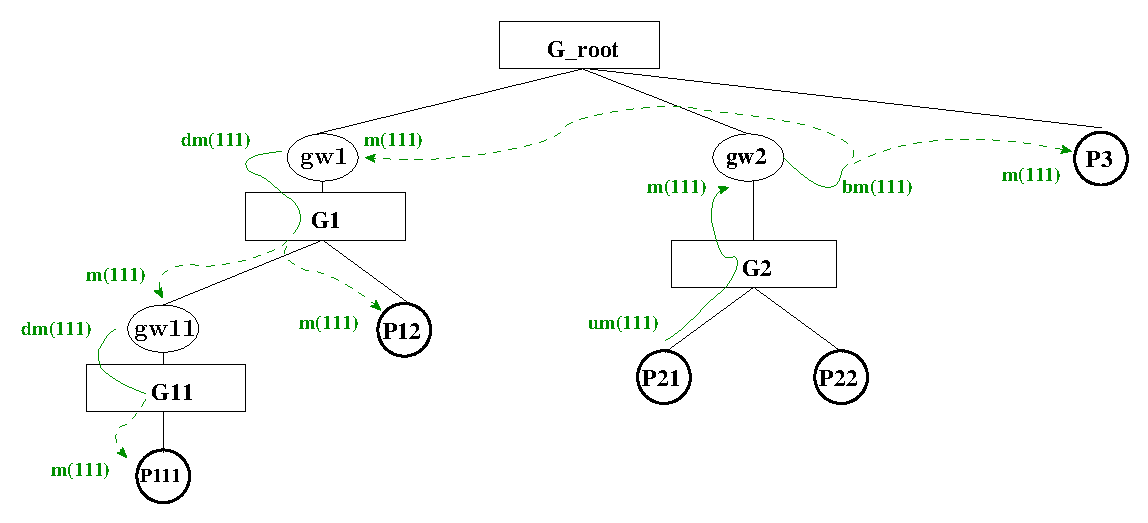
\includegraphics[width=0.9\linewidth]{XFIG/SchemaHB2}}
  \caption{Principle of a Hierarchical Broadcast structure and protocol}
  \label{fig:hb-scenario}
\end{figure}

Figure \ref{fig:hb-scenario} shows an instantiation of a HB
structure, and a possible scenario:
\begin{itemize}
\item
  The HB tree has 3 sub-groups, each with its gateway process, and 6
  processes scattered in the sub-groups.
\item
  The path in green shows the sequence of message exchanges when Process P21 (within
  group G2) sends a message to process P111 (within group G11).
\item
  As the target is not within the local group to which P21 belongs,
  the initial message $m(111)$ is sent up to group 2, and
  arrives in gateway $gw2$.
\item
  Now the destination belongs to a group that is a sibling of G2, so
  it is broadcast to all its siblings (sent as $bm(111)$, and
  received as $m(111)$). It will be simply discarded by
  gateways or processes that are not involved (here P3), while $gw1$
  will recognize as being of interest, and in next step send it down
  to its group.
\item
  Sending down is again a broadcast, to all members of sub-group
  G1. Process P12 will ignore it, while gateway $gw11$ in turn
  will recognize and forward the message.
\item
  Within group G11, process P111 will finally receives message
  $m(111)$, that terminates our scenario.
\end{itemize}

Along this paper, we will use this example to illustrate the use of
pNets as a structured semantic model, with a stress on the fact that
we represent here HB as a program schema, with unspecified process
arguments, using open pNets. We will show how the symbolic operational
semantics of open pNets computes the dynamics of the HB in term of a
symbolic representation that we call open-transitions, and how we can
prove equivalences between open systems.

\begin{example} \emph{First step: define the action algebra, with data domains,
    operators and predicates.}
  For our HB structure, we use send and receive messages encoded
  respectively as $m(arg)$ and $im(?var)$ with
  $arg$ of type \texttt{Address}. HB has a message-based
  structure, and by convention action names for action reception will
  be prefix by the letter "i". We abstract away
  from the payload of the messages, keeping only target addresses in the HB
  tree as an argument to all messages. Addresses are finite sequences
  of natural numbers written \texttt{s.i}
  with \texttt{s} a sequence and i a number. In concrete instantiations, we
  assume numbers are simple digits, and we write the sequences without
  the dot, as in ``121''. Then in the model of the
  gateways, we must be able to decide whether an address is below/above the
  current address, or in some specific relation, using
  predicates:\\
  - \emph{i==j} Syntactic equality between two sequences.\\
  - \emph{is\_ancestor(i,j)}: $i$ is a (strict) prefix of $j$.\\
  - \emph{is\_direct\_relative(i,j)}: $i$ and $j$ have a common prefix $k$, $i=k.i1$, $j=k.j1$, with $i1$ of length 1, but $j1$ can be of length equal or greater than 1 ($j$ is a brother or a nephew in the genealogy).\\
  - \emph{is\_other\_relative(i,j)}: all other cases.\\
  Note that these 4 predicates are exclusive.
\end{example}

\begin{example}  \emph{Second step: define the gateway behaviour as a pLTS.}

\begin{figure}[h]
\centerline{  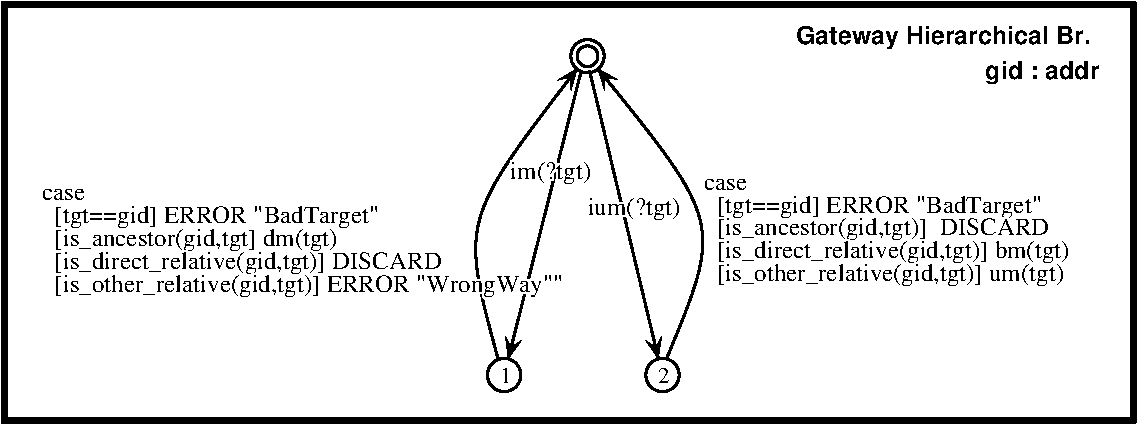
\includegraphics[width=0.85\linewidth]{ATG/GatewayHB}}
\caption{Behaviour of a Gateway controller %\TODO{ERIC: change the action syntax}
  }
  \label{fig:hb-HBgateway}
\end{figure}
Figure \ref{fig:hb-HBgateway} shows the pLTS representing the generic
gateway controller. From its initial state, it can receive messages
$ium(?tgt)$ from the subgroup below, or $im(?tgt)$
coming either from above or from an horizontal broadcast. The details will
be explained later, together with the model structure and the
protocol.
To simplify the notation in the pLTS drawings, we use the following
conventions: state variables are implicitely subscripted by the
adequate state number (e.g. $ium(?tgt)$ means $ium(?tgt_2)$), and we
have ``global'' variables that are defined in all states (here $gid$
means $gid_0,gid_1,gid_2$).

Note that we use \texttt{if-then-else} or \texttt{case}
constructs in the pLTS labels. These are mere abbreviations, that can
be expanded as a set of transitions carrying simple labels with adequate guards.
\end{example}

\begin{example} \emph{Sorts of pLTSs:}
  The sort of the gateway in Figure \ref{fig:hb-HBgateway} is:\\
  $\large\{ um(tgt_s), im(tgt_s), dm(tgt_s), bm(tgt_s), um(tgt_s),
  ium(tgt_s), DISCARD, \\ERROR(name) \large\}_{s\in\{1,2\}}$
\end{example}

\begin{figure}[t]
  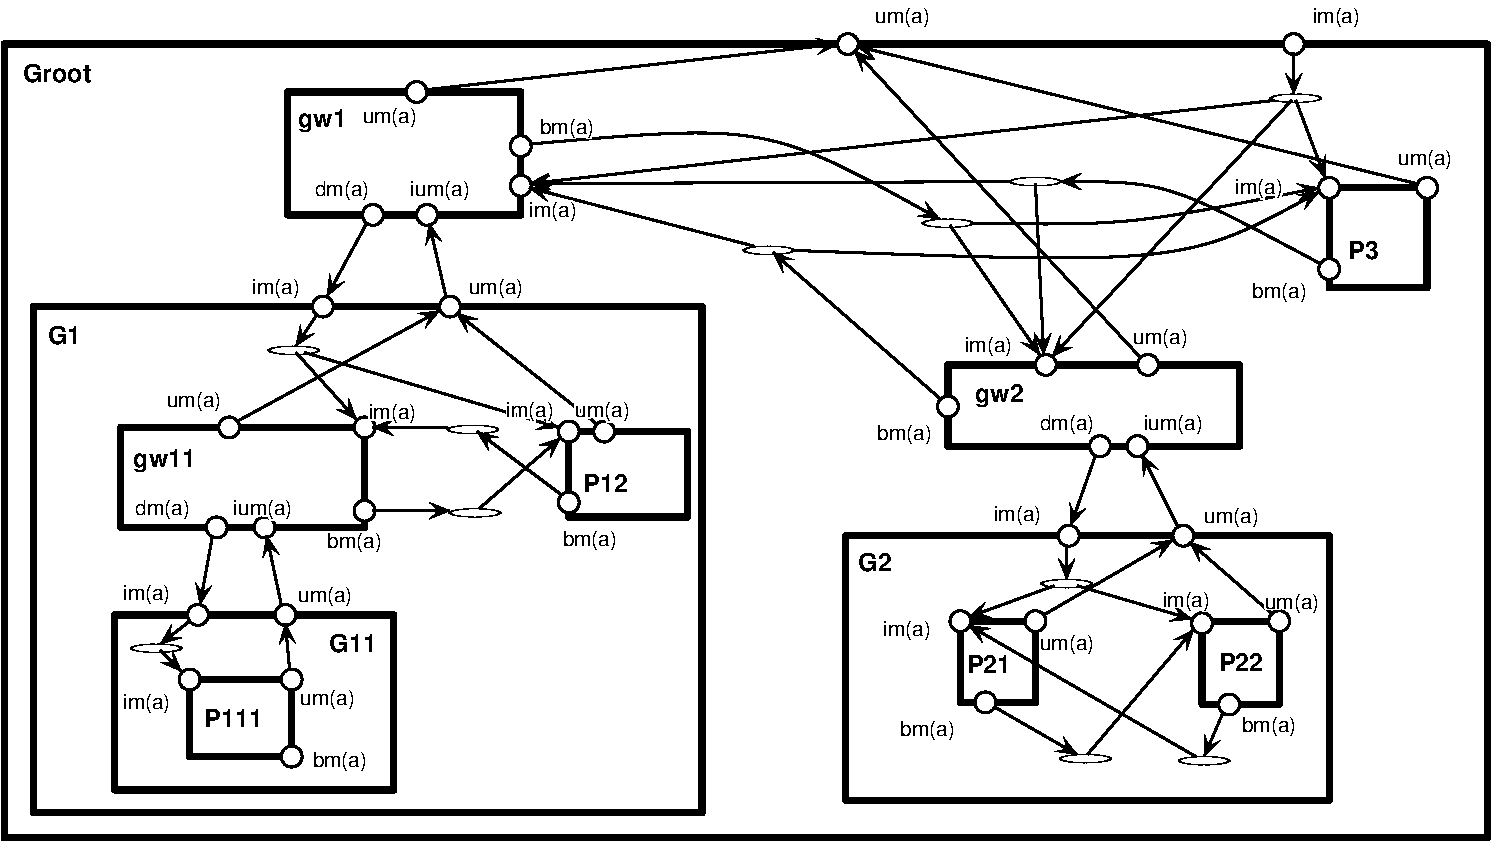
\includegraphics[width=1.0\linewidth]{ATG/Inst5}
  \caption{A Hierarchical Broadcast pNet Structure}\label{fig:hb-pnet-graphical}
 \end{figure}

\begin{example} \emph{pNet structure, and graphical representation}  
Here we show some parts of the pNet tree expressing our HB
structure. Figure \ref{fig:hb-pnet-graphical} shows the full pNet
model in a graphical format, where each box represents a pNet node
(Groot, G1, ..., G11), a pLTS (gw1, ..., gw11), or a process (P3, ...,
P111).
The actions in the sorts of the nodes appear as ports on the boxes,
and the synchronisation vectors as arrows, or multipoint ``webs''
drawn as ellipses. For
example, the webs
%labelled \texttt{tau}
in the Groot box
  correspond to synchronisation vectors expressing a broadcast
  communication from one of the subnets of Groot (gw1, gw2, or P3), to
  the others.

  Formally, the root pNet has a structure $<gw1, gw2, G1, G2, P3>$,
  with G1 and G2 sub-pNets, their associated gateways gw1, gw2
  pLTSs, and P3 a process Hole. We have 4 possible broadcast communications at the
  root, corresponding to as many synchronisation vectors; e.g. if gw2 is the sender:
  $< im(a), bm(a), -, -, im(a)> \to\!\underline{bm(a)}$.

  We define the synchronisation vectors in a parameterised way
  (independently of a specific HB network configuration) for any
  pNet node in a HB structure. Let $\widetilde{i}$ be the position of this pNet in the
  structure.
   We define here 4 of these synchronisation vectors, that we will
   use in the next sections to illustrate the semantic rules.
   %; the full table is listed in Appendix \ref{Appendix:SynchVectors}.
   In the
  vectors below,
  $\widetilde{I_G}=\{gw\widetilde{i}1,..,gw\widetilde{i}p,G\widetilde{i}1,..,G\widetilde{i}p\}$
   and
  $\widetilde{I_P}=\{P\widetilde{i}1,..,P\widetilde{i}p\}$ are the sets
  containing respectively the indexes of sub-nets and holes of the
  pNet node, $\widetilde{I_{G+P}}$ their union.

  \begin{figure}[h!]
  \label{fig:HBvectors}
  \begin{tabular}{|p{1.4cm}|p{11cm}|}
%% \hline\hline
%% \multicolumn{3}{|l|}{Hierarchical broadcasting}\\
  \hline
  \hline
$(UG)_{\widetilde{i}k}$\newline
 $k\leq g$&\raisebox{-2pt}{
 $\begin{array}[t]{@{}c@{}c@{}c@{}c@{}c@{}c@{}c@{}c@{}}
 &gw\widetilde{i}1,..&,gw\widetilde{i}k,&..,gw\widetilde{i}g,G\widetilde{i}1,..&,G\widetilde{i}k,&..,G\widetilde{i}g,P\widetilde{i}1,..,P\widetilde{i}p\\
<\!& -\,-\,-\    &  ,ium(\widetilde{t}),& -\ -\ -\  &,um(\widetilde{t}),&, -\ -\ -\
&\!>\longrightarrow \underline{um_{\widetilde{i}.k}(\widetilde{t})}
% $
%     \symb{sv}_{u(\widetilde{i}k)}\triangleq
%     <ium_{\widetilde{i}.k}(\widetilde{t})\otimes
%     -^{\widetilde{I_P}}\otimes
%     um_{\widetilde{i}.k}(\widetilde{t})\otimes
%  -^{{\widetilde{I_G}\backslash\{\widetilde{i}\cdot
%         k\}}}>\longrightarrow
%     \underline{um(\widetilde{t})}$
\end{array}$}  \raisebox{-19pt}{~}  \\
\hline
     &{\ERIC{Up gateway}: message m is sent
  up from a group to its gateway, received by the ium action. The
  resulting action is visible as the (synchronised) $\underline{um}$ }\\
\hline
 $(UM)_{\widetilde{i}k}$\newline$k\leq g$
 &\raisebox{-2pt}{$\begin{array}[t]{@{}c@{}c@{}c@{}c@{}c@{}c@{}c@{}c@{}}
 &gw\widetilde{i}1,..&,gw\widetilde{i}k,&..,gw\widetilde{i}g,G\widetilde{i}1,..,G\widetilde{i}g,P\widetilde{i}1,..,P\widetilde{i}p\\
 <\!& -\,-\,-\    &  ,um(\widetilde{t}),& -\ -\ -\   -\ -\ -\
 &\!>\longrightarrow \underline{um(\widetilde{t})}
 \end{array}$}\raisebox{-18pt}{~}\\
\hline
$(UM)_{\widetilde{i}k}$\newline$k\leq p$
&\raisebox{-2pt}{$\begin{array}[t]{@{}c@{}c@{}c@{}c@{}c@{}c@{}c@{}c@{}}
&gw\widetilde{i}1,..,gw\widetilde{i}g,G\widetilde{i}1,..,,G\widetilde{i}g,P\widetilde{i}1,..&,P\widetilde{i}k,&..,P\widetilde{i}p\\
<\!& -\ -\ -\      -\ -\ -\ &,um(\widetilde{t}),&   -\, -\, -
&\!>\longrightarrow \underline{um(\widetilde{t})}
\end{array}$}\raisebox{-18pt}{~}
 % &
%$\symb{sv}_{!\widetilde{i}}\triangleq
%    <um_{\widetilde{i}.k}(\widetilde{t})\otimes
%    -^{\widetilde{I_{G+P}}\backslash\{\widetilde{i}\cdot k\}}\otimes
%    -^{\widetilde{I_G}}>\longrightarrow
%    um_{\widetilde{i}.k}(\widetilde{t})$
\\
\hline
     &{\ERIC{Up Message}: message m is sent up from a process
  or a gateway to the enclosing (= parent) group}\\
\hline

%% $(BG)_{\widetilde{k}} \ERIC{HB}$ &
$(HB)_{\widetilde{i}k}$ \newline $k \leq g$
&\raisebox{-2pt}{$\begin{array}[t]{@{}c@{}c@{}c@{}c@{}c@{}c@{}c@{}c@{}}
&gw\widetilde{i}1,...&,gw\widetilde{i}k,&..,gw\widetilde{i}g,&G\widetilde{i}1,..,,G\widetilde{i}g&,P\widetilde{i}1,..,
P\widetilde{i}p \\
<\!& im(\widetilde{t}), .., im(\widetilde{t}) &, bm(\widetilde{t}),& im(\widetilde{t}),
..
im(\widetilde{t}),& -\ -\ -\  &,im(\widetilde{t}),..,im(\widetilde{t})
&\!>\longrightarrow \underline{bm(\widetilde{t})}
\end{array}$}\raisebox{-18pt}{~}
     \\
\hline
     &{\ERIC{Horizontal Broadcast}: message m, from a process or a
  gateway, is broadcast to all its siblings (processes and gateways)
  inside its group}\\
\hline\hline\end{tabular}
\caption{Synchronisation vectors modeling the communication through the HB hierarchy}
\end{figure}

\end{example}

  \begin{example}\emph{An open-transition.}\label{example:open-trans}
	After introducing the operational semantics rules, in example
        \ref{example:deduction-trees}, we shall explain how we 
	construct this transition using the rules.
	The transition below corresponds to the application of vector
        UG at position k=2, and gateway gw2 executing transition
        $0 \xrightarrow{ium(?tgt2_2)}_{gw2} 2$, storing some address in
        the state variable $tgt_2$ of gw2..
	
	\centerline{
		$\openrule
		{0 \xrightarrow{a}_{gw2} 2 \\
			\xrightarrow{b}_{P21}
			\\ \sm{Pred}_{Root} \\ \emptyset}
		{\ostate{000} \OTarrow{v} \ostate{020}}
		$
	}
	
	With the predicates
	
	$\Pred_{Root} = ( a \!=\! ium(?tgt2_2) \land b\!=\!um(t2) \land b\in
	\Sort_{P21} \land t2 = tgt2_2
	\land v \!= \! \underline{um(t2)} )  $
	In the broadcast examples, we do not use assignments and will omit the \Post part of 
	the open transition.
\end{example}

\begin{example} \emph{State of a pNet}
The pNet from Fig. \ref{fig:hb-pnet-graphical} has three leaves (gw1,
gw2, gw11). So its states will be tuples of length 3,
e.g. $\triangleleft 102 \triangleright$.
\end{example}

\begin{example} \emph{Using the operational rules to compute
    open-transitions}
  \label{example:deduction-trees}

To build a proof tree, we have to choose one synchronisation vector at
each instantiation of rule Tr2, and one pLTS transition at each
instantiation of rule Tr1. Each stage in the proof tree builds one
open-transition of the corresponding pNet node.  Let us explain in
detail the first two steps of the
scenario from Fig. \ref{fig:hb-scenario}:

\begin{figure}[h]
\centerline{ 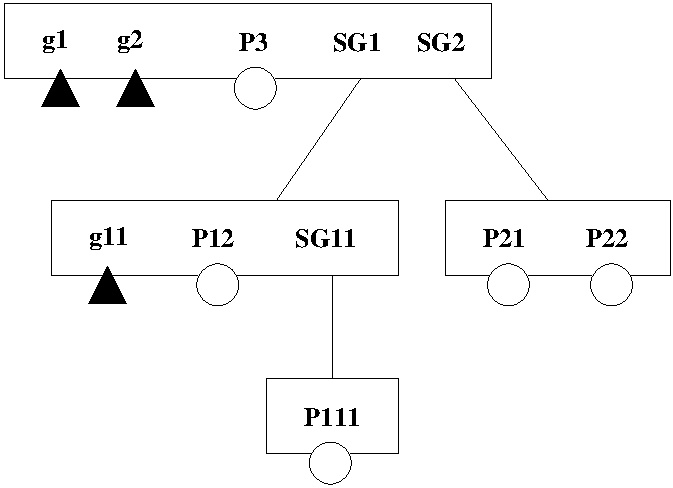
\includegraphics[width=5cm]{XFIG/HB2} }
\caption{(open) simplified pNet structure of Hierarchical Broadcast example}
\label{fig:flattening}
\end{figure}

\begin{itemize}
\item Process P21 sends a message towards P111, the combination of sync vectors UM\_21/UG\_2 conveys this message to gateway gw2.
\item The target address is a relative of gateway gw2, so it
  broadcasts the message to its siblings using vector HB\_2.
\end{itemize}
\end{example}

%% \TODO{but not for local variables of a given pLTS, that MUST keep their
%%   names through successive use, to keep the dataflow
%%   information. Still, of course, several instantiations of the same
%%   pLTS (like gw1, gw2) have distinct local varaibles.}

\paragraph{Building the first transition:}

We use instantiations of the synch vector UM at position 21 (that is a
hole), and of UG at position 2 (sub-group SG2 in the broadcast hierarchy) gives us :
\medskip


\noindent
UM\_21 : $< um(t1), - > \to\!um(t1)$\\
UG\_2 : $< -, ium(t2), -, -, um(t2) > \longrightarrow \underline{um(t2)}$

\smallskip\noindent
where the first synch vector (for sub-group SG2) has length 2, and the
second one (for the root pNet) has length 5. Using once the rule Tr1,
and twice rule Tr2, we build a proof tree, in which the premisses
define the behaviour of a gateway pLTS (here
$0 \xrightarrow{ium(?tgt2_2)}_{gw2} 2$, in which $tgt2_2$ stands for
the variable $tgt$ of state 2 in gw2), or of a process at a hole
(e.g. $\xrightarrow{b}_{P21}$ for the process at hole 21).
The conclusion is an open-transition of the root pNet, with the
composite state encoding the states of the 3 gateways at the Leaves,
e.g. $\ostate{000}$.




\begin{mathpar}
  \inferrule
      {\inferrule*
        {0 \xrightarrow{ium(?tgt2_2), True, \emptyset}_{gw2} 2}
        {\sm{gw2} \models
             \openrule {0 \xrightarrow{ium(?tgt2_2)}_{gw2} 2}
                       {\ostate{0} \xrightarrow{ium(?tgt2_2)} \ostate{2} }
             }
        \quad
        \inferrule* [right={[UM\_21]}]
           {
             %\sm{fresh}(b_{P21},v_{SG2})
           }
           {\sm{SG2} \models
             \openrule {\xrightarrow{b}_{P21} \quad \sm{Pred}_{UM\_21}}
                       {\ostate{-} \xrightarrow{v_{SG2}} \ostate{-} }
             }
%           \\ {\sm{fresh}(t1,t2,v) }
           \quad
           \sm{Pred}_{UG\_2}
      }
      {p\_Root
     \models
     \openrule
         {0 \xrightarrow{ium(?tgt2_2)}_{gw2} 2 \\
           \xrightarrow{b}_{P21}
          \\ \sm{Pred1}}
         {\ostate{000} \OTarrow{v} \ostate{020}}
      }      ~~ [UG\_2]
\end{mathpar}
With:

$Pred_{UM\_21} =  [um(t1)=b \land b\in \Sort_{P21} \land um(t1)=v_{SG2}]$

%% $Pred_{UG\_2} = [ium(?t2) = um(t2) \land v_{SG2} = um(t2) ]$

%% $Pred_{Root} = [ium(?t2) = ium(t2) \land b=um(t1) \land
%%   b\in \Sort_{P21} \land v_{SG2}=um(t1) \land v_{SG2} = um(t2)
%%   \land v = \tau]  $

$Pred_{UG\_2} = [ium(t2) = ium(?tgt2_2) \land um(t2) = v_{SG2} \land
  v = \underline{um(t2)} ]$

$Pred1 = [Pred_{UM\_21} \land Pred_{UG\_2}]  $

That can be simplified (eliminating the vector local variables and the
intermediate resulting actions), as: $Pred1 = [b\in \Sort_{P21}
  \land b=um(tgt2_2) \land v=\underline{b} ]  $

%% \TODO{Beware, problem with the ? of ?tgt2: I would prefer having no
%%   binder (? marker) in the open-automaton predicates, but I do not see
%% yet how the dataflow will be represented there. OOOOps no more input
%% var in this transition, t1 is a variable coming from P21.}



\section{Building more transitions of the HB example:}
\label{appendix:HB-tr2}
Here we detail the construction of the second transition of our
scenario:

\begin{mathpar}
     \openrule
         {0 \xrightarrow{im(?tgt1_1)}_{gw1} 1 \quad
           2 \xrightarrow{bm(tgt2_2)}_{gw2} 0 \quad
           \xrightarrow{b}_{P3}
           \quad Pred_{Root}}
         {\ostate{020} \OTarrow{v} \ostate{100}}
\end{mathpar}
with
$Pred_{Root} = [tgt1_1=tgt2_2 \land b=um(tgt2_2) \land
  b\in \Sort_{P3} \land v = \underline{bm(tgt2_2)}]  $

After the first move described in example \ref{example:deduction-trees}, the pLTS of $gw2$ is
in state 2, ready to emit. We build one
open-transition for each item in the case statement of its outgoing
transition; the one we are interested here for our scenario is the
case where the target address is below $gw1$, corresponding to the
predicate [$a$=$bm(tgt2_2)$ $\land$ isDirectRelative(2,$tgt2_2$)], and we
construct the proof tree, reduced here to applications of rule
Tr1 for transitions of the pLTSs gw1 and gw2, and a single application of rule
Tr2 for the synch vector HB at index 2:

\medskip\noindent
HB\_2 : $< im(t3), bm(t3), im(t3) -, - > \longrightarrow \underline{bm(t3)}$



This illustrates the flow of data through sequences of symbolic moves
of our example: in the first open-transition, the value (address) sent
by P21 was stored in the state variable $tgt2_2$. In the second
transition here, synchronisation within the vector HB\_2 yield the
predicate $tgt1_1=tgt2_2$, and thus transfers the address to the state
variable $tgt1_1$ in gw1.

\begin{mathpar}
  \inferrule
      {\inferrule
        {0 \xrightarrow{im(?tgt1_1)}_{gw1} 1}
        { \sm{gw1} \models
          \openrule
              {0 \xrightarrow{im(?tgt1_1)}_{gw1} 1 \quad \sm{True}}
              {\ostate{0} \OTarrow{im(?tgt1_1)} \ostate{1}}
        }
        \\
       \inferrule
           {2 \xrightarrow{bm(tgt2_2)}_{gw2} 0}
           { \sm{gw2} \models
             \openrule
                 {2 \xrightarrow{bm(tgt2_2)}_{gw2} 0 \quad \sm{Pred}_{gw2}}
                 {\ostate{2} \OTarrow{bm(tgt2_2)} \ostate{0}}
           }
           \quad Pred_{HB\_2}
      }
           {p\_Root
     \models
     \openrule
         {0 \xrightarrow{im(?tgt1_1)}_{gw1} 1 \quad
           2 \xrightarrow{bm(tgt2_2)}_{gw2} 0 \quad
           \xrightarrow{b}_{P3}
           \quad Pred2}
         {\ostate{020} \OTarrow{v} \ostate{100}}}
      ~~ [HB\_2]
\end{mathpar}

$Pred_{gw2} = [\sm{isDirectRelative}(2,tgt2_2)]$

$Pred_{HB\_2} = [im(tgt1_1) = im(t3) \land bm(tgt2_2) = bm(t3) \land b= im(t3) \land b\in 
\Sort_{P3}  \land v = \underline{bm(t3)}]$

$Pred2 = [Pred_{gw2} \land Pred_{HB\_2} ] $

\medskip
This can be simplified, eliminating the intermediate variable $t3$ of vector
HB\_2, while keeping the state variables of $gw_1$ and $gw_2$, the
intermediate $v$ created by Tr2, and the action variable of hole 
$P3$. This yields finally predicate $Pred2$ :

$Pred2 = [tgt1_1=tgt2_2 \land
  b\in \Sort_{P3} \land b=um(tgt2_2) \land v = \underline{bm(tgt2_2)}]
$

\medskip
Alternatively, we could also have elimated variable $v$, and directly
show the resulting action $\underline{bm(t3)}]$ in the open
  transition. This is slightly more compact, and maybe more readable,
  so we shall use this way in the open-automaton below.

\newpage
 
Below we show the initial transitions of the automaton of our HB
system. The full open-automaton has 17 states, and we have not
computed by hand its full set of transitions. This work would be very
tedious with pen and paper; we are currently developping a software
tool to this end.

\begin{figure}[h]
  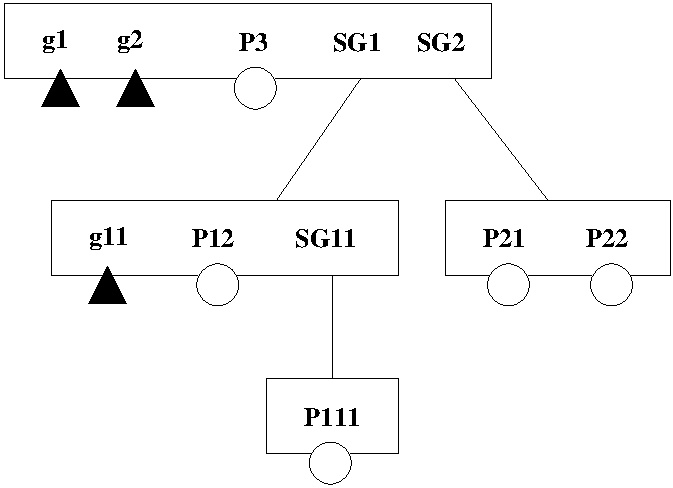
\includegraphics[width=0.35\linewidth]{XFIG/HB2}
\end{figure}

In this open-automaton, we have simplified the predicates and
eliminated the local variables, excepted those from the occurences of
the pLTS gw1 and gw2, and from the behaviour of holes.

\begin{figure}[h]
  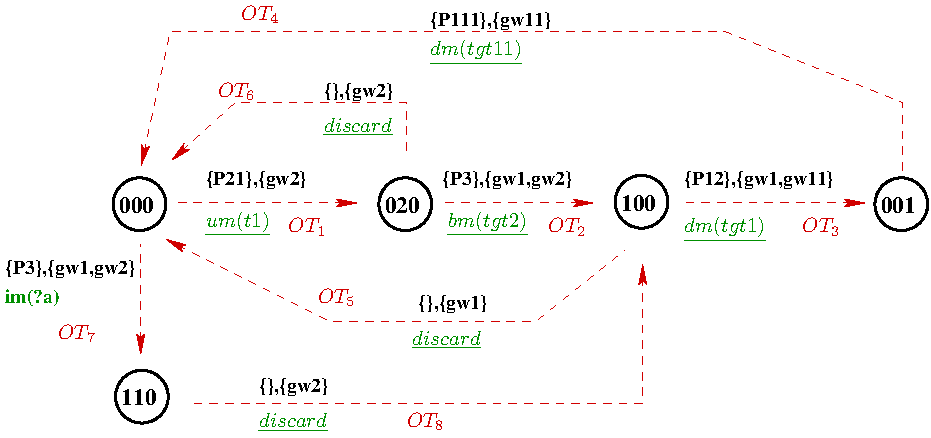
\includegraphics[width=\linewidth]{XFIG/HB-OpenAut}
\end{figure}
\newpage

\begin{eqnarray*}
OT_1 & = \openrule
         {0 \xrightarrow{ium(?tgt2)}_{gw2} 2 \quad
           \xrightarrow{b1}_{P21}
          \quad P1}
         {\ostate{000} \OTarrow{um(tgt2_2)} \ostate{020}}\\
 with & P1 = [b1\in \Sort_{P21} \land b1=um(tgt2_2) ]
 \\
OT_2 & = \openrule
         {0 \xrightarrow{im(?tgt1_1)}_{gw1} 1 \quad
           2 \xrightarrow{bm(tgt2_2)}_{gw2} 0 \quad
           \xrightarrow{b2}_{P3}
           \quad P2}
         {\ostate{020} \OTarrow{\underline{bm(tgt2_2)}} \ostate{100}}\\
         with & P2 = [tgt1_1=tgt2_2 \land IsDirectRelative(2,tgt2_2)
           \land  b2\in \Sort_{P3} \land b2=um(tgt2_2) ]
         \\
OT_3 & = \openrule
         {1 \xrightarrow{dm(tgt1_1)}_{gw1} 0 \quad
           0 \xrightarrow{im(?tgt11_1)}_{gw11} 1 \quad
           \xrightarrow{b3}_{P12}
           \quad P3}
         {\ostate{100} \OTarrow{\underline{dm(tgt1_1)}} \ostate{001}}\\
         with & P3 = [tgt11_1=tgt1_1 \land IsAncestor(1,tgt1_1)
           \land  b3\in \Sort_{P12} \land b3=im(tgt1_1) ]
         \\
OT_4 & = \openrule
         { 1 \xrightarrow{dm(tgt11_1)}_{gw11} 0 \quad
           \xrightarrow{b4}_{P111}
           \quad P4}
         {\ostate{001} \OTarrow{\underline{dm(tgt11)}} \ostate{000}}\\
 with & P4 = [ b4=im(tgt11_1) \land  b4\in \Sort_{P111} \land IsAncestor(11,tgt11_1) ]
         \\
OT_5 & = \openrule
         {1 \xrightarrow{Discard}_{gw1} 0 \quad
           \quad P5}
         {\ostate{100} \OTarrow{\underline{Discard}} \ostate{000}}\\
 with & P5 = [IsDirectRelative(1,tgt1_1) ]
 \\
OT_6 & = \openrule
         { 2 \xrightarrow{Discard}_{gw2} 0 \quad
           \quad P6}
         {\ostate{020} \OTarrow{\underline{Discard}} \ostate{000}}\\
 with & P6 = [ IsAncestor(2,tgt2_2) ]
 \\
OT_7 & = \openrule
         {0 \xrightarrow{im(?tgt1_1)}_{gw1} 1 \quad
          0 \xrightarrow{im(?tgt2_1)}_{gw2} 1 \quad
          \xrightarrow{b7}_{P3}\quad
           \quad P7}
         {\ostate{000} \OTarrow{im(?a)} \ostate{110}}\\
 with & P7 = [ tgt1_1 = tgt2_1 = a \land b7\in \Sort_{P3} \land b7 = im(?a)  ]
 \\
OT_8 & = \openrule
         {2 \xrightarrow{Discard}_{gw2} 0 \quad
           \quad P8}
         {\ostate{110} \OTarrow{Discard} \ostate{100}}\\
 with & P8 = [ IsDirectRelative(2,tgt2_1) ]
\end{eqnarray*}


\end{document}



\section{Discussion on substitution, matching, unification}


\TODO{this is far from being final... What should we leave here
  ? a generic definition of what must be part of the Action Algebra
  definition, substitution, protected variables; and
  move to other sections the application and examples of these.
In fact we currently do not use any notion of substitution, nor
protect variables. Only these predicates, built as sets of equations,
with a lot of fresh variables...}

\ERIC{[this text in blue is NOT supposed to stay here as such. Just
    guidelines towards identifying what we need to set up]
  To define the operational semantics of pNets, we need only two core
operations on action expressions: specialisation and unification.
\begin{itemize}
\item when composing pNets, substituting a pNet for a hole, each action in
the subnet sort has to match one action of the hole sort, but may be
more specific (substitution).
\item when building a proof tree from a synch vector, we collect a
  number of substitutions from the involved processes, and we have to
  match them with the action expressions in the vector. The result is
  a substitution for the variables of the global action, together with
  a predicate, built from the guards of the controllers and predicates
  of the subnets.
\end{itemize}
In some cases, substitutions are results of full unification between
action expressions, but in other cases it may be disymetric in the
sense that some variables can be substituted, and other not. We can
formalise this in term of ``protected variables'' in the unification,
opposed to ``input variables'' that can be arbitrarily substituted (=
can accept any value, like in classical value-passing algebra communication).}

\section{Future papers...}


I removed from here all appendices that were not directly related to this paper.
They will be providing subjects for future research (internships ?) and future papers, including:

\begin{itemize}
  \item Is open (strong) bisim compatible with pNet composition operator (as defined in PdP paper) ?
  \item Is Open-bisimulation compatible with closed bisimulation ?
    \item Effective algorithm for 1) checking strong bisimulation (given a state partition) 2) computing the coarsest partition (if it exists).
\item Model-checking Open-Automata:
This may come to be simpler to define and implement than FH-bisimulation.
\item FH-Refinement (and maybe even weak bisimulation if we do not find the time and/or space to have it here)
\item Fulll use-case on Hierarchical Broadcast
\end{itemize}




\section{Full definition of the HB pNet model}
\label{Appendix:SynchVectors}

  The table in Fig. \ref{fig:HBvectors} lists the synchronisation
  vectors used in all 3 algorithms and their variants. The vector
  naming schema is the following: the first letter encodes the direction
  of the message: U(p), D(own), H(orizontal); the second letter its
  type: B(roadcast) G(gateway-group) or M(simple message).

  Additionally, there are 2 special vectors, DIS for (silent) Discard
  events, and ERR for (visible) Error events.

  Among the 6 basic vectors, 3 of them (UG, DG, UM) are shared by all
  algorithms, DB is used by Full and hierarchical braodcast, while the
  last 2, HM and HB are specific to horizontal messages of Unicats and
  hierarchical brodcast respectively.

  \TODO{missing the variants here...}

\begin{figure}[h!]
  \label{fig:HBvectors}
\begin{tabular}{|p{1.6cm}|p{8.8cm}|l|}
%% \hline\hline
%% \multicolumn{3}{|l|}{Hierarchical broadcasting}\\
  \hline
  \hline
\multicolumn{3}{|p{12cm}|}{\ERIC{Need a short explanation about notations here: indices, indexed actions to be instanciated to match the terms in the sorts, ...? }}\\
  \hline
 %% $(UC)_{\widetilde{k}} \ERIC{UG}$ & $
 $(UG)_{\widetilde{k}}$ & $
     \symb{sv}_{u(\widetilde{i}.k)}\triangleq
     <?um_{\widetilde{i}.k}(\widetilde{t})\otimes
     -^{\widetilde{I_P}}\otimes
     !m_{\widetilde{i}.k}(\widetilde{t})\otimes
     -^{{\widetilde{I_G}\backslash\{\widetilde{i}\cdot
         k\}}}>\longrightarrow \tau(
     m_{\widetilde{i}.k}(\widetilde{t}))$ &
     $\widetilde{k}=\widetilde{i}.k\in \widetilde{I_G}$\\
\hline
     &\multicolumn{2}{|p{10cm}|}{\ERIC{Up gateway}: message m is sent up from a group to its gateway}\\
\hline
%% $(DG)_{\widetilde{k}} \ERIC{DB}$&
$(DB)_{\widetilde{k}}$&
$\symb{sv}_{?\widetilde{i}}\triangleq
     <?m_{\widetilde{i}.k}(\widetilde{t})\otimes
     -^{\widetilde{I_{G+P}}\backslash\{\widetilde{i}\cdot k\}}\otimes
     -^{\widetilde{I_G}}>\longrightarrow
     ?dm_{\widetilde{i}}(\widetilde{t})$&$\widetilde{k}=\widetilde{i}.k\in \widetilde{I_{G+P}}$\\
     \hline
     &\multicolumn{2}{|p{10cm}|}{\ERIC{Down Broadcast}: a message m received by a group is
       forwarded (broadcast) to all elements of the group, meaning to
       all processes and gateways inside.}\\
\hline
$(UM)_{\widetilde{k}}$&
$\symb{sv}_{!\widetilde{i}}\triangleq
    <!um_{\widetilde{i}.k}(\widetilde{t})\otimes
    -^{\widetilde{I_{G+P}}\backslash\{\widetilde{i}\cdot k\}}\otimes
    -^{\widetilde{I_G}}>\longrightarrow
    !um_{\widetilde{i}.k}(\widetilde{t})$ & $\widetilde{k}=\widetilde{i}.k\in \widetilde{I_{G+P}}$\\
\hline
     &\multicolumn{2}{|p{10cm}|}{\ERIC{Up Message}: message m is sent up from a process
  or a gateway to the enclosing (= parent) group}\\
\hline

%% $(BG)_{\widetilde{k}} \ERIC{HB}$ &
$(HB)_{\widetilde{k}}$ &
$\symb{sv}_{b(\widetilde{i}.k)}\triangleq
    <?m_{\widetilde{i}.j}^{\forall j\in I_K}(\widetilde{t})
    \otimes !bm_{\widetilde{i}.k}(\widetilde{t})
    \otimes -^{\widetilde{I_G}}>\longrightarrow \tau( bm(\widetilde{t}))$ &
    $I_K = \{k/\widetilde{i}.k\in \widetilde{I_{G+P}}\}$, \\ &  &  and
    $\widetilde{k}=\widetilde{i}.k$ \\
\hline
     &\multicolumn{2}{|p{10cm}|}{\ERIC{Horizontal Broadcast}: message m, from a process or a
  gateway, is broadcast to all its siblings (processes and gateways)
  inside its group}\\

\hline
%% $(DC)_{\widetilde{k}} \ERIC{DG}$ &
$(DG)_{\widetilde{k}}$ &
$\symb{sv}_{?\widetilde{i}}\triangleq
     <!dm_{\widetilde{i}.k}(\widetilde{t})\otimes
     -^{\widetilde{I_P}}\otimes
     ?dm_{\widetilde{i}.k}(\widetilde{t})\otimes
     -^{{\widetilde{I_G}\backslash\{\widetilde{i}\cdot k\}}}
     >\longrightarrow
     \tau(m_{\widetilde{i}.k}(\widetilde{t}))$,
%      <?m_{\widetilde{i}.k}^{\forall k\in
%        I_K}(\widetilde{t})\otimes
%      -^{\widetilde{I_P}}\otimes -^{\widetilde{I_G}}>\longrightarrow
     %      ?m_{\widetilde{i}}(\widetilde{t})$
     & $\widetilde{k}=\widetilde{i}.k\in \widetilde{I_G}$\\

\hline
     &\multicolumn{2}{|p{10cm}|}{\ERIC{Down Gateway}: message $m$ is sent down from a gateway
to the corresponding subgroup; it should then be forwarded inside the
subgroup, e.g. with $(DM)_{\widetilde{k}}$}\\
\hline
%% $(DK)_{\widetilde{k}} \ERIC{DM}$&
$(DM)_{\widetilde{k}}$&
$\symb{sv}_{!\widetilde{i}}\triangleq
    <  ?m_{\widetilde{i}.k}(\widetilde{t})\otimes
    -^{\widetilde{I_{G+P}}\backslash\{\widetilde{i}\cdot k\}}\otimes
    -^{\widetilde{I_G}}>\longrightarrow ?m_{\widetilde{i}}(\widetilde{t})$
    & $\widetilde{k}=\widetilde{i}.k\in \widetilde{I_{G+P}}$\\
\hline
     &\multicolumn{2}{|p{10cm}|}{\ERIC{Down Message}: Unicast version of (DB): m received
  by a group is forwarded to one specific element $i.k$ of the group}\\
\hline

$(HM)_{\widetilde{k}}$&
$\symb{sv}_{!\widetilde{i}}\triangleq
   $\\
\hline
&\multicolumn{2}{|p{10cm}|}{\ERIC{Horizontal Message}: optimized
  version of Unicast: message m, from a process or a
  gateway, is broadcast to one of its its siblings
  inside the same group}\\


\hline\hline
$(DIS)_{\widetilde{k}}$&
     $\symb{sv}_{u(\widetilde{i}.k)}\triangleq
     <Discard\otimes
     -^{\widetilde{I_{G+P}}\backslash\{\widetilde{i}\cdot k\}}\otimes
     -^{{\widetilde{I_G}\backslash\{\widetilde{i}\cdot
         k\}}}>\longrightarrow \tau(DIS)$ &
     $\widetilde{k}=\widetilde{i}.k\in \widetilde{I_G}$\\
\hline
     &\multicolumn{2}{|p{10cm}|}{\ERIC{DISCARD events} occur in gateways
  under HB protocol, after receiving a broadcast message which
  target address is a sibling of the gateway; this message is
  DISCARDED silently }\\
\hline
$(ERR)_{\widetilde{k}}$&
     $\symb{sv}_{u(\widetilde{i}.k)}\triangleq
     <Error\otimes
     -^{\widetilde{I_{G+P}}\backslash\{\widetilde{i}\cdot k\}}\otimes
     -^{{\widetilde{I_G}\backslash\{\widetilde{i}\cdot
         k\}}}>\longrightarrow Error(\widetilde{k})$ &
     $\widetilde{k}=\widetilde{i}.k\in \widetilde{I_G}$\\
\hline
     &\multicolumn{2}{|p{10cm}|}{\ERIC{ERROR events} may occur in gateways
  in 2 cases: either if the message is targeted to a gateway address,
  that is an error from the emittor (ERR "BadTarget"); or if a gateway
  receives from its parent or brother a message that should not go
  within its subgroup, that is a protocol error (ERR "WrongWay").
  In both cases the ERR message will be transmitted up, for the sake
  of verification }\\
\hline\hline\end{tabular}
\caption{Synchronisation vectors modeling the communication through the HB hierarchy}
\end{figure}

\section{The  Open Transitions of Broadcasting}
% \TODO{Min: to modify the tables. }

%%mofication of Table 1

\begin{figure}[h]
\centerline{ 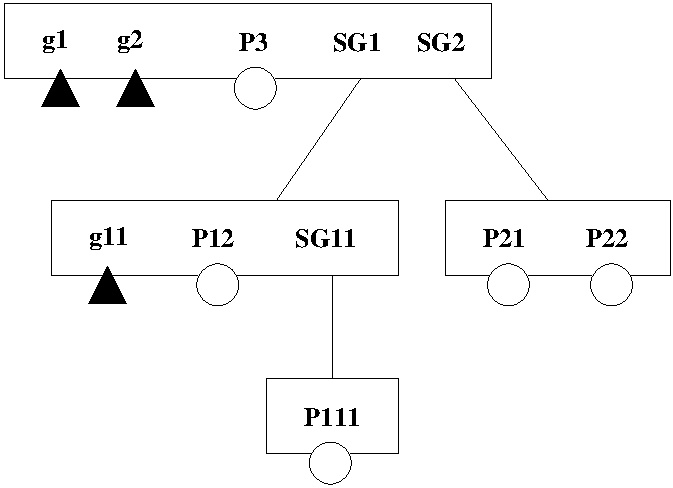
\includegraphics[width=5cm]{XFIG/HB2} }
\caption{(open) pNet structure of Hierarchical Broadcast example}
\label{Fig:simpleHBStruct}
\end{figure}

Figure \ref{Fig:simpleHBStruct} recalls the structure of the pNet tree
for HB example structure, in which gw1, gw2, gw11 are leaves, and P3,
P12, P21, P22, P111 are holes.

The following tables list the open-transition derivable from two of
the first states of the open-automaton of this pNet, including the 2 first
transitions of our scenario, as explained in section \ref{}.

\noindent
\begin{tabular}{|p{2.8cm}|p{9cm}|l|}
\hline\hline
\multicolumn{3}{|l|}{from state $\ostate{000}$}\\
\hline
HB(3) &
\{gw1, gw2\} \{P3\}  \{$a_{gw1}$=$a_{gw2}$=?m(t), $b_{P3}$=!bm(t'), v=$\tau$,[t=t']\} &
$\ostate{110}$\\
\hline
HB(12)&
\{gw11\} \{P12\} \{$a_{gw11}$=?m(t), $b_{P12}$=!bm(t'), v=$\tau$, [t=t' ]\} & $\ostate{001}$\\
\hline
DB&
\{gw1, gw2\}\{\}\{$a_{gw1}$=$a_{gw2}$=?m(t), v=?dm(t'),  [t=t']\}&$\ostate{110}$\\
\hline
UG(1)(UM(12)) &
\{gw1\},  \{P12\} \{$a-{gw1}$=?um(t), $b_{P12}$=!um(t'), v=$\tau$, [t=t']\} &
$\ostate{200}$\\
\hline
UG(2)(UM(k)) ${}^{k \in \{21,22\}}$ &
\{gw2\},  \{Pk\} \{$a_{gw2}$=?um(t), $b_{Pk}$=!um(t'),v=$\tau$, [t=t']\} &
$\ostate{020}$\\
\hline
UG(11)(UM(111)) &
\{gw11\},  \{P111\} \{$a_{gw11}$=?um(t), $b_{P111}$=!m(t),v=$\tau$, [t=t']\} &
$\ostate{002}$\\
\hline\hline
\end{tabular}
\vskip 0.3cm


\NOTE{Eric: one transition of the <020> table, from the draft on my white board}

\noindent
\begin{tabular}{|p{2.8cm}|p{9cm}|l|}
\hline\hline
\multicolumn{3}{|l|}{from state <020>}\\
\hline
HB(2)&
\{gw1,gw2\} \{P3\} \{a1=?m(t), a2=!bm(t'), a3=?m(t'), v=tau, [t=t'=t'' $\land$ isDirRel(t,2)]\} & <100>\\
\hline
HB(12)&
\{gw11\} \{P12\} \{a11=?m(t), a12=!bm(t'),  v=tau, [t=t']\} & <021>\\
\hline
UG(1)(UM(12)) &
\{gw1\},  \{P12\} \{a1=?um(t), a12=!um(t'), v=tau,  [t=t'] \} &
<220>\\
\hline
UG(11)(UM(111)) &
\{gw11\},  \{P111\} \{a11=?um(t), P111=!m(t),v=tau, [t=t']\} &
<022>\\
\hline
ERR(2)&
\{g2\} \{\} \{a2=Error, v=Error2,[t=2]\}&<000>\\
\hline
DiS(2)&
\{g2\} \{\} \{a2=DIS, v=DIS2,[Ancestor(2, t)]\} &
<000>\\
\hline
\hline
\end{tabular}
\vskip 0.3cm


%
%\noindent
%\begin{tabular}{|p{2.2cm}|p{9cm}|l|}
%\hline\hline
%\multicolumn{3}{|l|}{from state <1, 1, 0>}\\
%\hline
%HB(12)&
%\{g11\} \{P12\} \{a11=?m(a), a12=!bm(a), v=tau\} & <1, 1, 1>\\
%\hline
%UM(k) ${}^{k \in \{3,12\}}$&
%\{\}\{Pk\}\{ak=!um(a),v=!um(a), isOtherRelative(3, a)\}&<1, 1, 0>\\
%\hline
%UM(1)&
%\{g1\}\{\}\{a1=!um(a),v=!um(a), isOtherRelative(1, a)\}&<0, 1, 0>\\ \hline
%UM(2)&
%\{g2\}\{\}\{a2=!um(a),v=!um(a), isOtherRelative(2, a)\}&<1, 0, 0>\\ \hline
%DG(1)&
%\{g1\}\{SG1\}\{a1=!dm(a),sg1=?dm(a),v=tau\}&<0, 1, 0>\\ \hline
%DG(2)&
%\{g2\}\{SG2\}\{a2=!dm(a),sg2=?dm(a), v=tau\}&<1, 0, 0>\\ \hline
%
%DIS(1)&
%\{g1\} \{\} \{a1=Discard, v=tau\} &
%<0, 1, 0>\\
%\hline
%DIS(2)&
%\{g2\} \{\} \{a2=Discard, v=tau\} &
%<1, 0, 0>\\
%\hline
%ERR(1)&
%\{g1\} \{\} \{a1=Error, v=Error1\}, &
%<0, 1, 0>\\
%\hline
%ERR(2)&
%\{g2\} \{\} \{a2=Error, v=Error2\} &
%<1, 0, 0>\\
%\hline
%UG(11) &
%\{g11\},  \{SG11\} \{a11=?um(a), sg11=!m(a),v=tau, isOtherRelative(11, a)\} &
%<1, 1, 2>\\
%\hline\hline
%\end{tabular}
%\vskip 0.3cm
%\noindent
%\begin{tabular}{|p{2.2cm}|p{9cm}|l|}
%\hline\hline
%\multicolumn{3}{|l|}{from state <0, 0, 1>}\\
%\hline
%HB(3) &
%\{g1, g2\} \{P3\} \hfill \{a1=a2=?m(a), a3=!bm(a), v=tau\} &
%<1, 1, 1>\\
%\hline
%DB &
%\{g1, g2\} \{\} \{a1=a2=?m(a), v=?dm(a)\} &
%<1, 1, 1>\\
%\hline
%UG(1) &
%\{g1\},  \{SG1\} \{a1=?um(a), sg1=!m(a),v=tau, isOtherRelative(1, a)\} &
%<2, 0, 1>\\
%\hline
%UG(2) &
%\{g2\},  \{SG2\} \{a2=?um(a), sg2=!m(a),v=tau, isOtherRelative(2, a)\} &
%<0, 2, 1>\\
%\hline
%DG(11)  &
%% $\emptyset$
%\{g11\} \{SG11\} \{a11=!dm(a),sg11=?dm(a) v=tau,\} & <0, 0, 0>\\
%\hline
%
%DIS11 &
%\{g11\},\{\}\{a11=Discard, v=tau \}&<0, 0, 0>\\
% \hline
% ERR11 &
%\{g11\},\{\}\{a11=Error, v=Error11 \}&<0, 0, 0>\\
% \hline\hline
%\end{tabular}
%
%\vskip 0.3cm
%There is the case of Unicast.
%\vskip 0.3cm
%\noindent
%\begin{tabular}{|p{2.2cm}|p{9cm}|l|}
%\hline\hline
%\multicolumn{3}{|l|}{from state <0, 0, 0>}\\
%\hline
%DM1 &
%\{g1\} \{P3\}  \{a1=?m(a), a3=!m(a), v=tau, isDirectRelative(1,a)\} &
%<1, 0, 0>\\
%\hline
%DM2 &
%\{g2\} \{P3\}  \{a1=?m(a), a3=!m(a), v=tau, isDirectRelative(2,a)\} &
%<0, 1, 0>\\
%\hline
%DM11 &
%\{g11\} \{P13\}  \{a11=?m(a), a13=!m(a), v=tau, isDirectRelative(11,a)\} &
%<0, 0, 1>\\
%\hline\hline
%\end{tabular}
%\vskip 0.3cm
%\noindent
%\begin{tabular}{|p{2.2cm}|p{9cm}|l|}
%\hline\hline
%\multicolumn{3}{|l|}{from state <1, 0, 0>}\\
%\hline
%DG1 &
%\{g1\} \{SG1\}  \{a1=!dm(a), sg1=?dm(a), v=tau, isDirectRelative(1,a)\} &
%<0, 0, 0>\\
%\hline
%UM1 &
%\{g1\} \{\}  \{a1=!um(a), v=!um(a)\} &
%<0, 0, 0>\\
%\hline
%DM2 &
%\{g2\} \{P3\}  \{a1=?m(a), a3=!m(a), v=tau, isDirectRelative(2,a)\} &
%<1, 1, 0>\\
%\hline
%DM11 &
%\{g11\} \{P13\}  \{a11=?m(a), a13=!m(a), v=tau, isDirectRelative(11,a)\} &
%<1, 0, 1>\\
%\hline
%ERR(1)&
%\{g1\} \{\} \{a1=Error, v=tau\} &
%<0, 0, 0>\\
%\hline\hline
%\end{tabular}
%
%\vskip 0.3cm
%
%\noindent
%\begin{tabular}{|p{2.2cm}|p{9cm}|l|}
%\hline\hline
%\multicolumn{3}{|l|}{from state <1, 1, 0>}\\
%\hline
%DG1 &
%\{g1\} \{SG1\}  \{a1=!dm(a), sg1=?dm(a), v=tau, isDirectRelative(1,a)\} &
%<0, 1, 0>\\
%\hline
%DG2 &
%\{g2\} \{SG2\}  \{a2=!dm(a), sg2=?dm(a), v=tau, isDirectRelative(2,a)\} &
%<1, 0, 0>\\
%\hline
%UM1 &
%\{g1\} \{\}  \{a1=!um(a), v=!um(a)\} &
%<0, 1, 0>\\
%\hline
%UM2 &
%\{g2\} \{\}  \{a2=!um(a), v=!um(a)\} &
%<1, 0, 0>\\
%\hline
%DM11 &
%\{g11\} \{P13\}  \{a11=?m(a), a13=!m(a), v=tau, isDirectRelative(11,a)\} &
%<1, 1, 1>\\
%\hline
%ERR(1)&
%\{g1\} \{\} \{a1=Error, v=tau\} &
%<0, 1, 0>\\
%\hline
%ERR(2)&
%\{g2\} \{\} \{a2=Error, v=tau\} &
%<1, 0, 0>\\
%\hline\hline
%\end{tabular}


\section{Encapsulating Process arguments}
In Section \ref{section:processSort} we described the Sort of
processes in the holes of the herarchical broadcast architecture.
Here we present a more general solution, using a small pNet as a
filter encapsulating each of the holes. The filter is in
 charge of relabeling the messages
from the process depending on their destination, and filtering the
incoming messages, discarding those received by broadcast, but target
to other processes. This pNet is shown in the following figure:

\centerline{  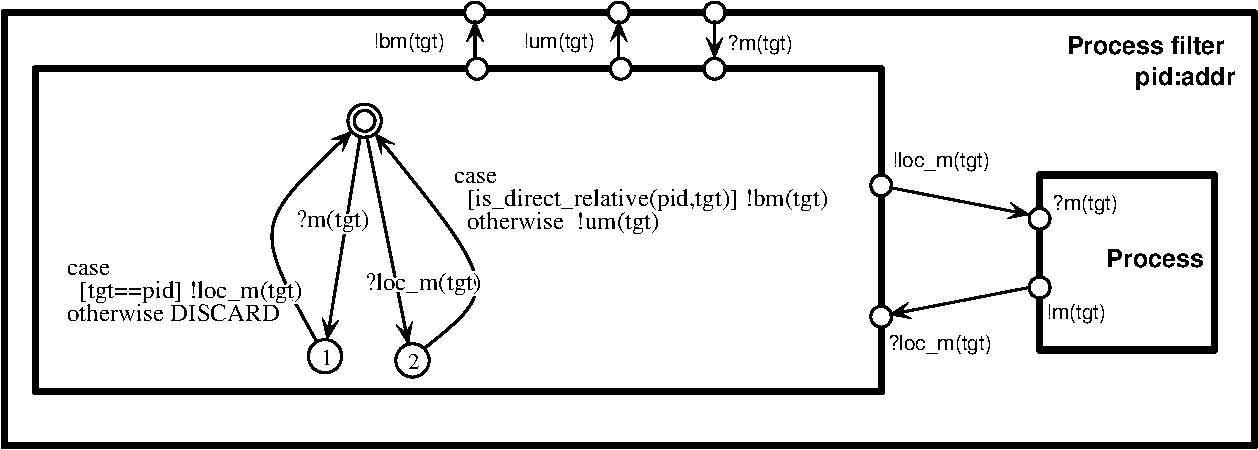
\includegraphics[width=0.8\linewidth]{ATG/ProcessFilter}}

This solution has the benefit of allowing any process as an argument
fitting the hole, without specific constraints on its sort. The price
is that the pNet structure is a bit more complex, so the open
transitions and open automata will be bigger also. Moreover the filter
has states, and this introduces some additional states and
tau-transitions in the open-automaton.


\section{{pNets Model for Broadcast Flat groups  (BF-pNets):
    definition}\label{sec:bf-pnets-def}}
Given a $HB-\pNet$, we can flatten it to decrease the number of layers
of hierarchical structures using a {\em Flattening Operator}
$\bowtie$.
This operation replaces one or several subgroups in the hierarchical
structure by their content. The corresponding old controllers
(gateways) won't exist after flattening. Fig. \ref{fig:flattening}
shows the flattening operator at work, on 2 subgroups SG1 and SG2, at the
toplevel of the example.
\begin{definition}[Flattening Operation]
Assume a $HB-\pNet$ has the structure:
$\mylangle gw_{\widetilde{g}}^{\widetilde{g}\in \widetilde{I_G}},  pc_{\widetilde{p}}^{\widetilde{p}\in \widetilde{I_P}}, sg_{\widetilde{g}}^{\widetilde{g}\in \widetilde{I_G}}\myrangle$
where
$ \forall \widetilde{g}\in \widetilde{I_G}$,  the $sg_{\widetilde{g}}$ has the $HB-\pNet$ structure:
 $\mylangle gw_{\widetilde{g}\cdot g_i}^{g_i\in I_{G_{\widetilde{g}}}},  pc_{\widetilde{g}\cdot p_j}^{p_j\in I_{P_{\widetilde{g}}}}, sg_{\widetilde{g}\cdot g_i}^{g_i\in I_{G_{\widetilde{g}}}}\myrangle $.
 \medskip

 Then
the flattening map
$\bowtie_{\widetilde{g}}: HB-pNets\longrightarrow HB-pNets$, where\\

 \medskip
 $\bowtie_{\widetilde{g}}(HB-\pNet)\triangleq \mylangle gw_{\widetilde{g}}^{\widetilde{g}\in \widetilde{I_G}\setminus\{\widetilde{g}\}}, gw_{\widetilde{g}\cdot g_i}^{g_i\in I_{G_{\widetilde{g}}}},  pc_{\widetilde{p}}^{\widetilde{p}\in \widetilde{I_P}}, pc_{\widetilde{g}.\cdot p_j}^{p_j\in I_{P_{\widetilde{g}}}},sg_{\widetilde{g}}^{\widetilde{g}\in \widetilde{I_G}\setminus\{\widetilde{g}\}}, sg_{\widetilde{g}\cdot g_i}^{g_i\in I_{G_{\widetilde{g}}}}\myrangle$.
 \medskip


The flattening operator shows one subgroup $sg_{\widetilde{g}}$ can be flatten to one hole of his father group which is linked the gateway $gw_{\widetilde{g}}$, the gateways,the processes ,and the holes of $sg_{\widetilde{g}}$ become the gateways, the processes, and the holes of his father group instead of itself and the gateway that it is linked.

Actually, for any subgroup (hole) of the group, the flattening operation can be done in parallel without the order.
We denote that  $\bowtie_{\widetilde{I_G}}\triangleq\Sigma_{\widetilde{g}\in{\widetilde{I_G}}}\bowtie_{\widetilde{g}}$, where:

 $\bowtie_{\widetilde{I_G}}(HB-\pNet)\triangleq \mylangle  gw_{\widetilde{g}\cdot g_i}^{\widetilde{g}\in \widetilde{I_G}, g_i\in I_{G_{\widetilde{g}}}},  pc_{\widetilde{p}}^{\widetilde{p}\in \widetilde{I_P}}, pc_{\widetilde{g}\cdot p_j}^{\widetilde{g}\in \widetilde{I_G}, p_j\in I_{P_{\widetilde{g}}}}, sg_{\widetilde{g}\cdot g_i}^{\widetilde{g}\in \widetilde{I_G}, g_i\in I_{G_{\widetilde{g}}}}\myrangle$.
\end{definition}

Especially, if some $\widetilde{g_0}\in{\widetilde{I_G}}$, the $sg_{\widetilde{g_0}}$ has the $HB-\pNet_{\widetilde{g_0}}$ structure: $\mylangle -,  pc_{\widetilde{g_0}\cdot p_j}^{p_j\in I_{P_{\widetilde{g}}}}, -\myrangle$.

 $\bowtie_{\widetilde{g_0}}(HB-\pNet)\triangleq \mylangle gw_{\widetilde{g}}^{\widetilde{g}\in \widetilde{I_G}\setminus\{\widetilde{g}\}},   pc_{\widetilde{p}}^{\widetilde{p}\in \widetilde{I_P}}, pc_{\widetilde{g_0}\cdot p_j}^{ p_j\in I_{P_{\widetilde{g}}}},sg_{\widetilde{g}}^{\widetilde{g}\in \widetilde{I_G}\setminus\{\widetilde{g}\}}\myrangle$.

% If all the subgroups $sg_{\widetilde{g}}$ have the similar structures to $sg_{\widetilde{g_0}}$, $\forall \widetilde{g}\in \widetilde{I_G}$, we have
%
%  $\bowtie_{\widetilde{I_G}}(HB-\pNet)\triangleq \mylangle -,  pc_{\widetilde{p}}^{\widetilde{p}\in \widetilde{I_P}}, pc_{\widetilde{g}\cdot p_j}^{\widetilde{g}\in \widetilde{I_G}, p_j\in I_{P_{\widetilde{g}}}}, -\myrangle$.

\medskip
%
%\begin{definition}[Equivenlence]
%\NOTE{The equivalence between $HB-\pNet$ and $BF-\pNet$ should be defined.}
%\end{definition}


 Let $HB-\pNet$ node have the structure $\mylangle gw_{\widetilde{g}}^{\widetilde{g}\in \widetilde{I_G}},  pc_{\widetilde{p}}^{\widetilde{p}\in \widetilde{I_P}}, sg_{\widetilde{g}}^{\widetilde{g}\in \widetilde{I_G}}\myrangle$, with some subgroup the $sg_{\widetilde{g_0}}$ who has the  structure:
 $\mylangle gw_{\widetilde{g_0}\cdot g_i}^{g_i\in I_{G_{\widetilde{g_0}}}},  pc_{\widetilde{g_0}\cdot p_j}^{p_j\in I_{P_{\widetilde{g_0}}}}, sg_{\widetilde{g_0}\cdot g_i}^{g_i\in I_{G_{\widetilde{g_0}}}}\myrangle $, has one corresponding flatten broadcast open $\pNet$ by the flattening operator $\bowtie_{\widetilde{g_0}}$, i.e. $\mylangle gw_{\widetilde{g}}^{\widetilde{g}\in \widetilde{I_G}\setminus\{\widetilde{g_0}\}}, gw_{\widetilde{g_0}\cdot g_i}^{g_i\in I_{G_{\widetilde{g}}}},  pc_{\widetilde{p}}^{\widetilde{p}\in \widetilde{I_P}}, pc_{\widetilde{g_0}.\cdot p_j}^{p_j\in I_{P_{\widetilde{g}}}},sg_{\widetilde{g}}^{\widetilde{g}\in \widetilde{I_G}\setminus\{\widetilde{g_0}\}}, sg_{\widetilde{g_0}\cdot g_i}^{g_i\in I_{G_{\widetilde{g}}}}\myrangle$.



\section{Sketch of the proof}
\label{sec:proof-sketch}

In this section we will describe a proof of equivalence between a HB
pNet node (seen as an open pNet), with the corresponding flatten
broadcast open pNet. From this equivalence, it is easy to derive the
equivalence of a fully instantiated (= closed) HB-pNet structure with
the corresponding flatten pNet.

\begin{theorem}
Any $\mathcal{HB-\pNet}$ node is FH-bisimular to the corresponding $\mathcal{BF-\pNet}$ node by the flatting operator $\bowtie$, that is, \\
$\mylangle gw_{\widetilde{g}}^{\widetilde{g}\in \widetilde{I_G}},  pc_{\widetilde{p}}^{\widetilde{p}\in \widetilde{I_P}}, sg_{\widetilde{g}}^{\widetilde{g}\in \widetilde{I_G}\setminus\{\widetilde{g_0}\}},\mylangle gw_{\widetilde{g_0}\cdot g_i}^{g_i\in I_{G_{\widetilde{g_0}}}},  pc_{\widetilde{g_0}\cdot p_j}^{p_j\in I_{P_{\widetilde{g_0}}}}, sg_{\widetilde{g_0}\cdot g_i}^{g_i\in I_{G_{\widetilde{g_0}}}}\myrangle  \myrangle \approx_{FH} \\ \mylangle gw_{\widetilde{g}}^{\widetilde{g}\in \widetilde{I_G}\setminus\{\widetilde{g_0}\}}, gw_{\widetilde{g_0}\cdot g_i}^{g_i\in I_{G_{\widetilde{g}}}},  pc_{\widetilde{p}}^{\widetilde{p}\in \widetilde{I_P}}, pc_{\widetilde{g_0}.\cdot p_j}^{p_j\in I_{P_{\widetilde{g}}}},sg_{\widetilde{g}}^{\widetilde{g}\in \widetilde{I_G}\setminus\{\widetilde{g_0}\}}, sg_{\widetilde{g_0}\cdot g_i}^{g_i\in I_{G_{\widetilde{g}}}}\myrangle$.
\end{theorem}

The sketch we give here considers one particular pNet node, with 2
subgroups, and a specific number of processes in each root- and sub-
groups. Also we make some hypotheses on the sorts of the processes.
Clearly the full proof will have to deal with generalisations of this
particular case.

\begin{figure}[h]
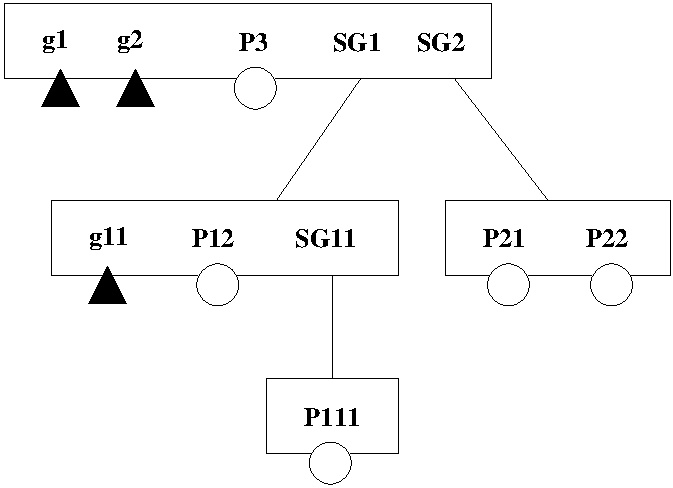
\includegraphics[width=6cm]{XFIG/HB2}
\hspace{1cm}
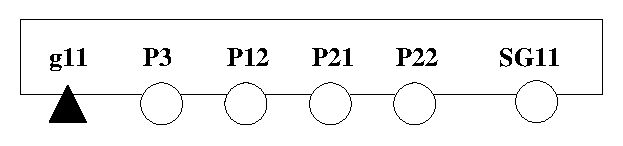
\includegraphics[width=5cm]{XFIG/B2}
\caption{(open) pNet structure of Hierarchical and flat example}
\label{fig:flattening}
\end{figure}

\paragraph{More precisely:}

\paragraph{Principles of the proof:}

We start from the hierarchical pNet, build all its possible behaviours
(building proof trees from possible synch vectors of the pNet, and
possible actions in the sorts of holes), then show that there is a
corresponding behaviour for the flat pNet. Similar method is then
applied in the symetrical direction.

A state of the hierarchical pNet will be a hierarchical vector of
``states'', in which we shall represent the state of a controller with
its name followed by the state index (gateways have only two states,
numered \{0,1\}); and state of holes with simply the name of the hole.
To keep state structure compact and keep readability, we show pLTS
states by their number, subscripted by the name of the gateway. For
processes and sub-groups, that have no states, we only show their name.
%
%
%
%\noindent
%\begin{tabular}{|p{2.2cm}|p{9cm}|l|}
%\hline\hline
%\multicolumn{3}{|l|}{from state <0, 0, 0>}\\
%\hline
%Bm(3) &
%\{g1, g2\} \{P3\} \hfill \{a1=a2=?bm(a), a3=!m(a), v=tau\} &
%<1, 1, 0>\\
%\hline
%Bm(12)&
%\{g11\} \{P12,P13\} \{a11=a13=?um(a), a12=!m(a), v=tau\} & <0, 0, 1>\\
%\hline
%Bm(13)&
%\{g11\} \{P12,P13\} \{a11=a12=?um(a), a13=!m(a), v=tau\} & <0, 0, 1>\\
%\hline
%DA &
%\{g1, g2\} \{P3\} \{a1=a2=a3=?bm(a), v=?m(a)\} &
%<1, 1, 0>\\
%\hline
%Um(1) &
%\{g1\},  \{SG1\} \{a1=?bm(a), sg1=!m(a),v=tau, isOtherRelative(1, a)\} &
%<2, 0, 0>\\
%\hline
%Um(2) &
%\{g2\},  \{SG2\} \{a2=?bm(a), sg2=!m(a),v=tau, isOtherRelative(2, a)\} &
%<0, 2, 0>\\
%\hline
%Um(11) &
%\{g11\},  \{SG11\} \{a11=?bm(a), sg11=!m(a),v=tau, isOtherRelative(11, a)\} &
%<0, 0, 2>\\
%\hline
%UA(k) ${}^{k \in \{3,12,13,21\}}$ &
%% $\emptyset$
%\{\} \{Pk\} \{ak=!um(a), v=!m(a)\} & <0, 0, 0>\\
%\hline\hline
%\end{tabular}
%
%\noindent
%\begin{tabular}{|p{2.2cm}|p{9cm}|l|}
%\hline\hline
%\multicolumn{3}{|l|}{from state <1, 1, 0>}\\
%\hline
%Bm(12)&
%\{g11\} \{P12,P13\} \{a11=a13=?um(a), a12=!m(a), v=tau\} & <1, 1, 1>\\
%\hline
%Bm(13)&
%\{g11\} \{P12,P13\} \{a11=a12=?um(a), a13=!m(a), v=tau\} & <1, 1, 1>\\
%\hline
%UA(3)&
%\{\}\{P3\}\{a3=!um(a),v=!m(a), isOtherRelative(3, a)\}&<1, 1, 0>\\
%\hline
%UA(1)&
%\{g1\}\{\}\{a1=!um(a),v=!m(a), isOtherRelative(1, a)\}&<0, 1, 0>\\ \hline
%UA(2)&
%\{g2\}\{\}\{a2=!um(a),v=!m(a), isOtherRelative(2, a)\}&<1, 0, 0>\\ \hline
%$Dm_1(DA_1)$ &
%\{g1,g11\}\{SG1,P12,P13\}\{a1=!dm(a), sg1=?m(a),a11=a12=a13=?bm(a), v=tau, isDirectRelative(1,a)\}&<0, 1, 1>\\ \hline
%$Dm_2(DA_2)$ &
%\{g2\}\{SG2,P21\}\{a2=!dm(a), sg2=?m(a), a21=?bm(a), v=tau, isDirectRelative(2,a)\}&<1, 0, 0>\\ \hline
%DISCARD(1)&
%\{g1\} \{\} \{a11DISCARD, v=tau\} &
%<0, 1, 0>\\
%\hline
%DISCARD(2)&
%\{g2\} \{\} \{a2=DISCARD, v=tau\} &
%<1, 0, 0>\\
%\hline
%Um(11) &
%\{g11\},  \{SG11\} \{a11=?bm(a), sg11=!m(a),v=tau, isOtherRelative(11, a)\} &
%<1, 1, 2>\\
%\hline\hline
%\end{tabular}
%\begin{tabular}{|p{2.2cm}|p{9cm}|l|}
%\hline\hline
%\multicolumn{3}{|l|}{from state <0, 0, 1>}\\
%\hline
%Bm(3) &
%\{g1, g2\} \{P3\} \hfill \{a1=a2=?bm(a), a3=!m(a), v=tau\} &
%<1, 1, 1>\\
%\hline
%DA &
%\{g1, g2\} \{P3\} \{a1=a2=a3=?bm(a), v=?m(a)\} &
%<1, 1, 1>\\
%\hline
%Um(1) &
%\{g1\},  \{SG1\} \{a1=?bm(a), sg1=!m(a),v=tau, isOtherRelative(1, a)\} &
%<2, 0, 1>\\
%\hline
%Um(2) &
%\{g2\},  \{SG2\} \{a2=?bm(a), sg2=!m(a),v=tau, isOtherRelative(2, a)\} &
%<0, 2, 1>\\
%\hline
%UA(k) ${}^{k \in \{3,12,13,21\}}$ &
%% $\emptyset$
%\{\} \{Pk\} \{ak=!um(a), v=!m(a)\} & <0, 0, 1>\\
%\hline
%UA(11)  &
%% $\emptyset$
%\{g11\} \{\} \{a11=!um(a), v=!m(a)\} & <0, 0, 0>\\
%\hline
%Dm(11)&
%\{g11\},\{SG1\},\{a11=!dm(a),sg11=?m(a), v=tau, isDirectRelative(11,a)\}&<0, 0, 0>\\
%\hline
%DISCARD &
%\{g11\},\{\}\{a11=DISCARD, v=tau, isOtherRelative(11,a) \}&<0, 0, 0>\\ \hline\hline
%\end{tabular}
%\begin{tabular}{|p{2.2cm}|p{9cm}|l|}
%\hline\hline
%\multicolumn{3}{|l|}{from state <2, 0, 0>}\\
%\hline
%Bm(12) &
%\{g11\} \{P12,P13\}  \{a11=a12=?bm(a), a13=!m(a), v=tau\} &
%<2, 0, 1>\\
%\hline
%Bm(13) &
%\{g11\} \{P12,P13\}  \{a11=a13=?bm(a), a12=!m(a), v=tau\} &
%<2, 0, 1>\\
%\hline
%Bm(1) &
%\{g1,g2\} \{P3\}  \{a2=a3=?bm(a), a1=!m(a), v=tau\} &
%<0, 1, 0>\\
%\hline
%Um(2) &
%\{g2\},  \{SG2\} \{a2=?bm(a), sg2=!m(a),v=tau, isOtherRelative(2, a)\} &
%<2, 2, 0>\\
%\hline
%UA(k) ${}^{k \in \{3,12,13,21\}}$ &
%% $\emptyset$
%\{\} \{Pk\} \{ak=!um(a), v=!m(a)\} & <2, 0, 0>\\
%\hline
%UA(1)  &
%% $\emptyset$
%\{g1\} \{\} \{a1=!um(a), v=!m(a)\} & <0, 0, 0>\\
%\hline
%Um(11)&
%\{g11\}\{SG11\}\{a11=?um(a), sg11=!m(a), v=tau, isOtherRelative(11,a)\}&<2, 0, 2>\\
%\hline
%DISCARD(1) &
%\{g1\},\{\},\{a1=DISCARD, v=tau, isDirectRelative(1,a)\}&<0, 0, 0>\\
%\hline\hline
%\end{tabular}
%\begin{tabular}{|p{2.2cm}|p{9cm}|l|}
%\hline\hline
%\multicolumn{3}{|l|}{from state <0, 2, 0>}\\
%\hline
%Bm(12) &
%\{g11\} \{P12,P13\}  \{a11=a12=?bm(a), a13=!m(a), v=tau\} &
%<0, 2, 1>\\
%\hline
%Bm(13) &
%\{g11\} \{P12,P13\}  \{a11=a13=?bm(a), a12=!m(a), v=tau\} &
%<0, 2, 1>\\
%\hline
%Bm(2) &
%\{g1,g2\} \{P3\}  \{a1=a3=?bm(a), a2=!m(a), v=tau\} &
%<1, 0, 0>\\
%\hline
%Um(1) &
%\{g1\},  \{SG1\} \{a1=?bm(a), sg1=!m(a),v=tau, isOtherRelative(2, a)\} &
%<2, 2, 0>\\
%\hline
%UA(k) ${}^{k \in \{3,12,13\}}$ &
%% $\emptyset$
%\{\} \{Pk\} \{ak=!um(a), v=!m(a)\} & <0, 2, 0>\\
%\hline
%UA(2)  &
%% $\emptyset$
%\{g2\} \{\} \{a2=!um(a), v=!m(a)\} & <0, 0, 0>\\
%\hline
%DISCARD(2)&
%\{g2\},\{\},\{a2=DISCARD, v=tau, isDirectRelative(2,a)\}&<0, 0, 0>\\
%\hline
%Um(11) &
%\{g11\},\{SG11\}\{a11=?um(a), sg11=!m(a), v=tau, isOtherReltive(11, a) \}&<0, 2, 2>\\ \hline\hline
%\end{tabular}
%\begin{tabular}{|p{2.2cm}|p{9cm}|l|}
%\hline\hline
%\multicolumn{3}{|l|}{from state <0, 0, 2>}\\
%\hline
%Bm(3) &
%\{g1, g2\} \{P3\} \hfill \{a1=a2=?bm(a), a3=!m(a), v=tau\} &
%<1, 1, 2>\\
%\hline
%DA &
%\{g1, g2\} \{P3\} \{a1=a2=a3=?bm(a), v=?m(a)\} &
%<1, 1, 2>\\
%\hline
%Um(1) &
%\{g1\},  \{SG1\} \{a1=?bm(a), sg1=!m(a),v=tau, isOtherRelative(1, a)\} &
%<2, 0, 2>\\
%\hline
%Um(2) &
%\{g2\},  \{SG2\} \{a2=?bm(a), sg2=!m(a),v=tau, isOtherRelative(2, a)\} &
%<0, 2, 2>\\
%\hline
%UA(k) ${}^{k \in \{3,12,13,21\}}$ &
%% $\emptyset$
%\{\} \{Pk\} \{ak=!um(a), v=!m(a)\} & <0, 0, 2>\\
%\hline
%UA(11)  &
%% $\emptyset$
%\{g11\} \{\} \{a11=!um(a), v=!m(a)\} & <0, 0, 0>\\
%\hline
%Bm(11)&
%\{g11\},\{P12,P13\},\{a11=!m(a),a12=a13=?bm(a), v=tau, \}&<0, 0, 0>\\
%\hline
%DISCARD(11)&
%\{g11\},\{\}\{a11=DISCARD, v=tau, isDirectRelative(11,a) \}&<0, 0, 0>\\ \hline\hline
%\end{tabular}
%\begin{tabular}{|p{2.2cm}|p{9cm}|l|}
%\hline\hline
%\multicolumn{3}{|l|}{from state <1, 1, 1>}\\
%\hline
%UA(1)&
%\{g1\}\{\}\{a1=!um(a),v=!m(a), isOtherRelative(1, a)\}&<0, 1, 1>\\
%\hline
%UA(2)&
%\{g2\}\{\}\{a2=!um(a),v=!m(a), isOtherRelative(2, a)\}&<1, 0, 1>\\
%\hline
%UA(3)&
%\{\}\{P3\}\{a3=!um(a),v=!m(a), isOtherRelative(3, a)\}&<1, 1, 1>\\
%\hline
%Dm(11)&
%\{g11\}\{SG11\}\{a11=!dm(a), sg11=?m(a), v=tau, isDirectRelative(11,a)\}&<1, 1, 0>\\ \hline
%$Dm_2(DA_2)$ &
%\{g2\}\{SG2,P21\}\{a2=!dm(a), sg2=?m(a),a21=?bm(a), v=tau, isDirectRelative(2,a)\}&<1, 0, 1>\\ \hline
%DISCARD(1)&
%\{g1\} \{\} \{a1=DISCARD, v=tau, isOtherRelative(1,a)\} &
%<0, 1, 1>\\
%\hline
%DISCARD(2)&
%\{g2\} \{\} \{a2=DISCARD, v=tau, isOtherRelative(2,a)\} &
%<1, 0, 1>\\
%\hline
%DISCARD(11)&
%\{g11\} \{\} \{a11=DISCARD, v=tau, isOtherRelative(11,a)\} &
%<1, 1, 0>\\
%\hline\hline
%\end{tabular}
%\begin{tabular}{|p{2cm}|p{9cm}|l|}
%\hline\hline
%\multicolumn{3}{|l|}{from state <0, 1, 0>}\\
%\hline
%Bm(12) &
%\{g11\} \{P12,P13\}  \{a11=a12=?bm(a), a13=!m(a), v=tau\} &
%<0, 1, 1>\\
%\hline
%Bm(13) &
%\{g11\} \{P12,P13\}  \{a11=a13=?bm(a), a12=!m(a), v=tau\} &
%<0, 1, 1>\\
%\hline
%Um(1) &
%\{g1\},  \{SG1\} \{a1=?um(a), sg1=!m(a),v=tau, isOtherRelative(1, a)\} &
%<2, 1, 0>\\
%\hline
%Um(11) &
%\{g11\},  \{SG11\} \{a11=?um(a), sg1=!m(a),v=tau, isOtherRelative(11, a)\} &
%<0, 1, 2>\\
%\hline
%UA(k) ${}^{k \in \{3,12,13\}}$ &
%% $\emptyset$
%\{\} \{Pk\} \{ak=!um(a), v=!m(a)\} & <0, 1, 0>\\
%\hline
%UA(2)  &
%% $\emptyset$
%\{g2\} \{\} \{a2=!um(a), v=!m(a)\} & <0, 0, 0>\\
%\hline
%$Dm_2(DA_2)$ &
%\{g2\},\{SG2,P21\},\{a2=!dm(a),sg2=?m(a),a21=?bm(a) v=tau, isDirectRelative(2,a)\}&<0, 0, 0>\\
%\hline
%DISCARD(2) &
%\{g2\},\{\}\{a2=DISCARD, v=tau, isOtherRelative(2,a) \}&<0, 0, 0>\\ \hline\hline
%\end{tabular}
%\begin{tabular}{|p{2cm}|p{9cm}|l|}
%\hline\hline
%\multicolumn{3}{|l|}{from state <1, 0, 0>}\\
%\hline
%Bm(12) &
%\{g11\} \{P12,P13\}  \{a11=a12=?bm(a), a13=!m(a), v=tau\} &
%<1, 0, 1>\\
%\hline
%Bm(13) &
%\{g11\} \{P12,P13\}  \{a11=a13=?bm(a), a12=!m(a), v=tau\} &
%<1, 0, 1>\\
%\hline
%DISCARD &
%\{g1\} \{\}  \{a1=DISCARD),  v=tau, isOtherRelative(1,a)\} &
%<0, 0, 0>\\
%\hline
%Um(2) &
%\{g2\},  \{SG2\} \{a2=?bm(a), sg2=!m(a),v=tau, isOtherRelative(2, a)\} &
%<1, 2, 0>\\
%\hline
%Um(11) &
%\{g11\},  \{SG11\} \{a11=?bm(a), sg11=!m(a),v=tau, isOtherRelative(11, a)\} &
%<1, 0, 2>\\
%\hline
%UA(k) ${}^{k \in \{3,21\}}$ &
%% $\emptyset$
%\{\} \{Pk\} \{ak=!um(a), v=!m(a)\} & <1, 0, 0>\\
%\hline
%UA(1)  &
%% $\emptyset$
%\{g1\} \{\} \{a1=!um(a), v=!m(a)\} & <0, 0, 0>\\
%\hline
%$Dm_1(DA_1)$ &
%\{g1,g11\},\{SG1, P12, P13\},\{a1=!dm(a),sg11=?m(a), a11=a12=a13=?bm(a), v=tau, isDirectRelative(1,a)\}&<0, 0, 0>\\
%\hline
%DA(1) &
%\{g11\},\{P12,P13\}\{a11=a12=a13=?bm(a), v=?m(a) \}&<1, 0, 0>\\ \hline\hline
%\end{tabular}
%\begin{tabular}{|p{2.2cm}|p{9cm}|l|}
%\hline\hline
%\multicolumn{3}{|l|}{from state <0, 1, 1>}\\
%\hline
%DISCARD(2) &
%\{g2\} \{\}  \{a2=DISCARD),  v=tau, isOtherRelative(2,a)\} &
%<0, 0, 1>\\
%\hline
%DISCARD(11) &
%\{g11\} \{\}  \{a11=DISCARD),  v=tau, isOtherRelative(11,a)\} &
%<0, 1, 0>\\
%\hline
%Um(1) &
%\{g1\},  \{SG1\} \{a1=?um(a), sg1=!m(a),v=tau, isOtherRelative(1, a)\} &
%<2, 1, 1>\\
%\hline
%UA(k) ${}^{k \in \{3,12,13\}}$ &
%% $\emptyset$
%\{\} \{Pk\} \{ak=!um(a), v=!m(a)\} & <0, 1, 1>\\
%\hline
%UA(2)  &
%% $\emptyset$
%\{g2\} \{\} \{a2=!um(a), v=!m(a)\} & <0, 0, 1>\\
%\hline
%$Dm_2(DA_2)$&
%\{g2\},\{SG2,P21\},\{a2=!dm(a),sg2=?m(a),a21=?bm(a), v=tau, isDirectRelative(2,a)\}&<0, 0, 1>\\
%\hline
%Dm(11)&
%\{g11\},\{SG11\},\{a11=!dm(a),sg11=?m(a), v=tau, isDirectRelative(11,a)\}&<0, 1, 0>\\
%\hline\hline
%\end{tabular}
%
%\noindent
%\begin{tabular}{|p{2cm}|p{9cm}|l|}
%\hline\hline
%\multicolumn{3}{|l|}{from state <0>}\\
%\hline
%Bm(3) &
%\{g11\} \{P3,P12,P13,P21\} \hfill \{a11=a12=a13=a21=?bm(a), a3=!m(a), v=tau\} &
%<1>\\
%\hline
%\multicolumn{2}{|l|}{Bm(12,13,21) are similar} & <1>\\
%\hline
%Um(11) &
%\{g11\} \{SG11\} \{a11=?um(a), sg11=!m(a), v=tau\} & <2>\\
%\hline
%DA &
%\{g11\} \{P3,P12,P13,P21\} \{a3=a11=a12=a13=a21=?bm(a), v=?m(a)\} &
%<1>\\
%\hline
%UA(k) ${}^{k \in \{3,12,13,21\}}$ &
%% $\emptyset$
%\{\} \{Pk\} \{ak=!um(a), v=!m(a)\} & <0>\\
%\hline\hline
%\multicolumn{3}{|l|}{from state <1>}\\
%\hline
%DISCARD&
%{g11} \{\} \hfill \{a11=DISCARD, v=tau, isDirectRelative(11,a)\} &
%<0>\\
%\hline
%UA(11)& \{g11\} \{\} \{a11=!um(a), v=!m(a), isOtherRelative(11,a)\}& <0>\\
%\hline
%UA(k) ${}^{k \in \{3,12,13,21\}}$ &
%\{\} \{Pk\} \{ak=!um(a), v=!m(a)\} & <1>\\
%\hline
%Dm(11)& \{g11\} \{SG11\} \{a11=!dm(a), sg11=?dm(a), v=tau, isAncestor(11,a)\} & <0>\\
%\hline\hline
%\multicolumn{3}{|l|}{from state <2>}\\
%\hline
%Bm(11) &
%{g11} \{P3,P12,P13,P21\} \hfill \{a11=!bm(a), a3=a12=a13=a21=?bm(a),
%v=tau, isDirectRelative(11,a)\} & <0>\\
%\hline
%UA(11) &
%{g11} \{\} \hfill \{a11=!um(a),
%v=!m(a), isOtherRelative(11,a)\} & <0>\\
%\hline
%UA(k) ${}^{k \in \{3,12,13,21\}}$ &
%\{\} \{Pk\} \{ak=!um(a), v=!m(a)\} & <2>\\
%\hline
%DISCARD &
%{g11} \{\} \hfill \{a11=DISCARD, v=tau, isAncestor(11,a)\} & <0>\\
%\hline\hline
%
%\end{tabular}

\section{Open-bisimulation is compatible with closed bisimulation ?}

\TODO{Underneath is the rules of the closed semantics. Not sure we
  should keep them here, but we mentionned we should have a proof of
  the relation between the 2 semantics... In an extended version I
  suppose (;-)}

\begin{mathpar}
    \inferrule{\phi,\phi',\phi''\!\in\!\Phi\\s \xrightarrow{\langle \alpha,~e_b,~(x_j\!:= {e}_j)^{j\in J}\rangle} s'\in \to\\\\
      \phi'\!=\!\phi\!+\!\{x'_i\!\to\!V_i|x'_i\!\in\!\iv(\alpha)\land V_i\!\in\!\mathcal{D}\} \\
      e_b\phi'\!=\!\symb{True} \\ \phi''\!=\!\phi'+\{x_j\!\to\! e_j\phi'|j\!\in\! J\}}
    {(s,\phi) \xrightarrow{\alpha\phi'} (s',\phi'') \in\llbracket\mylangle S,s_0,
      \to\myrangle\rrbracket_\Phi}~~{\bf Tr1}
%         \end{mathpar}
% \begin{mathpar}

    \inferrule {\phi,\phi'\in\Phi\\ \alpha_l^{l\in L} \to \alpha \in \overline{\symb{SV}}\\\forall i\in I\phi\setminus
      L\phi.\,s'_i=s_i
      \\ %\iv(\alpha)=(x_k)^{k\in K}\\\\
      \forall l\in L\phi.\,\phi_l\in\Phi\land s_l \xrightarrow{\alpha_l\phi_l} s'_l\in\llbracket\pNet_l\rrbracket_{\Phi}\\\phi'=\phi+\uplus_{l\in L\phi} \phi_{l} }
{\triangleleft s_i^{i\in I\phi}\triangleright \xrightarrow{\alpha\phi'} \triangleleft{s'_i}^{i\in
        I\phi'}\triangleright  \in \llbracket\mylangle \pNet_i^{i\in I},\emptyset,\overline{\symb{SV}}\myrangle\rrbracket_\Phi}~~{\bf Tr2}
\end{mathpar}


\section{Model Checking open-automata}
 \TODO{The following is about the logic formula}

We want to check (and prove) properties on open pNets, using
model-checking techniques on their open-automata. The properties will be
expressed in any version of (action-based) branching temporal logics,
in which we have to add constructs for quantification over the holes
and/or leaves involved in a transition. For simplicity of the
definition, we could choose here ACTL \cite{ACTL1990,ACTL1993} or ACTL*
\cite{DeNicolaVaandrager95}, or the modal $\mu$-calculus
\cite{Koz83}. Instead, for its easiness of
expression of value-passing calculi properties, we use here the {\em
  Model Checking Language} MCL \cite{MateescuFM2008}



\begin{definition}[FH-ACTL ] The logic formula of ACTL (adding  syntax
  for quantifying over open \pNet s : $\forall t\in {\cal{P}}, H_i \xrightarrow{a} H_i^\prime $)
\end{definition}

 \begin{definition}[FH-satisfiability] Suppose that $F$ is an open
   \pNet\ expression, and $\phi$ is a temporal logic formula, we say
   $F$ satisfies the $\phi$, denoted as   $F\vDash_{FH} \phi$,  if
 \end{definition}

 In a quite standard way, we define the model checking problem as
 satisfiability of an FH-ACTL formula in a state of a FH-automaton.
The specificity is that the model (FH-automaton) transitions include
hypotheses about which holes are involved and predicates about their
behaviours.

 \begin{definition}[The Open MC problem]
 \end{definition}

 \section{refinement}
 \begin{definition}[FH-refinement] FH-refinement relation $\ll$ is a
   binary relation in between open \pNet \ expressions iff for any
   open \pNet \ expressions $E$ and $F$, $E\ll F$, we have the
   follows:
 \begin{itemize}
 \item $\P(E)=\P(F)$;
 \item  For any  $E\xrightarrow{S, Pred, a} E'$ based on one open transition $(S, Pred, E')$ for $F$,   there exist a set indexed by $\{j\in J\}$ of transitions  $\{ F\xrightarrow{S_j, Pred_j, a\tau^\star} F_j^\prime| a=a' up\ to\ \alpha-conversation\}$  such that $\forall j\in J, S\subset S_j,  E'\ll F_j'$ and $Pred=\cup_j Pred_j$.
 \end{itemize}
 \end{definition}
 \begin{definition}[Weak FH-refinement] FH-refinement relation $\ll$ is a binary relation in between open \pNet \ expressions iff for any open \pNet \ expressions $E$ and $F$, $E\ll F$, we have the follows:
 \begin{itemize}
 \item $\P(F)=\P(E)$;
 \item  For any  $E\xrightarrow{S, Pred, a} E'$ based on one open transition $(S, Pred, E')$ for $E$,   there exist a set indexed by $\{j\in J\}$ of transitions  $\{ F\xRightarrow{(\uplus_i S_i)_j, (\cap_i Pred_i)_j, \tau^\star a'\tau^\star} F_j^\prime| F\xrightarrow{S_i, Pred_i, a'/\tau} F_i, a=a' up \ to \ \alpha-conversation\}$  such that $\forall j\in J, S=(\uplus_i S_i)_j, E'\ll F_j^\prime$  and $Pred \subseteq \cup_j(\cap_i Pred_i)_j$.
 \end{itemize}
 \end{definition}

 \begin{theorem} Suppose that two \pNet s expressions $E$ and $F$ where $E$ is strong FH-bisimilar to $F$. For any temporal logic formula $\phi$,  if $E\vDash_{FH}\phi$, then we have $F\vDash_{FH} \phi$.
 \end{theorem}

  \section{pNets Model for Hierarchical Broadcast groups  (HB-pNets): definition}\label{sec:b-pnets-def}

In this section, we give the formal model for the broadcast type of
hierarchical groups using our open parameterised networks (pNets).

Hierarchical Broadcast (HB) is a way of implementing broadcasting
algorithms within a large set of processes, with better performances
and scalability. There have been many proposals for hierarchical
broadcast algorithms (cite...), most of them focussing on specific
architectures or features (in particular fault tolerance), and on
performance analysis. Very few have given a formal description of the
algorithm, allowing to reason about their safety properties.

We give here the description of one simple HB algorithm, extracted
from\cite{Taguchi03}, but without fault
tolerance in a first step. For the formal description, we define a
pNet template, that can be used as a building node in a hierarchical
assembly of processes, organised in a tree of sub-groups; communication makes use
of local broadcast within each sub-group, and uses gateways for
transmission of messages, up and down, between the subgroups. The
gateways are described as generic pLTSs, playing the role of
``controllers'' in the pNet node.

\TODO{start with a simple informal description ?}

More precisely, we model a generic structure supporting
  hierarchical groups of processes, including gateways. Then
  we model 3 differents message
  routing algorithms, plus 2 variants, all working on this same
  network topology, namely:
\begin{itemize}
\item Full broadcast: the message goes up to the root of the
  tree, then is broadcasted down to all processes in all groups.
\item Hierarchical broadcast 1: similar to unicast, but within each
  subgroup the communication uses local broadcast. Only the processes
  in the same group than the target process will received the
  message.
This is the algorithm from the original paper \cite{Taguchi03}, in its
simplified version without fault tolerance mechanisms.
\item Hierarchical broadcast 2: same principle, but without horizontal broadcast between sibling processes and gateways: the message has to go up to the enclosing subgroup/gateway, before detecting it can go down to its target.
\item Unicast: the gateways forward the message using the shortest
  route in the tree. The message will reach only the specified target.
\item Unicast 2: same principle, but with detection of sibling situations, and direct sending of messages to sibling gateways/processes, thus shortening the path in a way similar to the Hierarchical Broadcast 1.
\end{itemize}

We will use these 3 algorithms, and their variants, to illustrate the
type of properties we can prove using open pNets and FH-bisimulations.
Note that we cannot hope to get any strong bisimulation equivalences
between them, the intermediate messages introduced by the protocoles
are different. To get interesting properties, we must hide
intermediate messages, and look for weak bisimulation properties.

Here are some examples:

\ERIC{Simple scenario: When hiding everything but send and receive
  messages from processes, the resulting systems with Unicast and
  Hierarchical broadcast are weak equivalent
  ?}

\ERIC{Hierarchical Broadcast Variants: when hiding all horizontal messages
  the two variants are Weak Equivalent ? (same for Unicast variants) }

\ERIC{What kind of relation with Full broadcast ? This is more tricky,
on one hand we have to abstract away from the target id in the
arguments of messages; then full broadcast is indeed broadcasting
everywhere, so the best we can hope is some refinement relation,
because Hierachical Broadcast has naturally less behaviours.}



Given a process configuration, organised hierarchicaly in subgroups,
it is easy to build a pNet tree reflecting the hierarchy, with the
gateways implementing the 3 algorithms. In the next
section, we will prove that this model of the implementation is indeed
equivalent (modulo weak bisimulation) to a flat broadcast.




\medskip


The whole broadcast mechanism of hierarchical groups consists in normal
processes, gateways and subgroups linked by gateways. Normal processes
can send and receive messages to/from the other processes (including
gateways) in the same group, or send up-messages to its enclosing group.

\TODO{Restructure these explanations}
A gateway has external behaviours : it sends down-messages to its associated
subgroup, and receives up-messages from its subgroup.
Gateways behaviour is defined by a simple pLTS with two or three states depending on the algorithm: in the
initial state the gateway can receive a
$?m(\widetilde{tgt})$ message (from its neighbors,
from the enclosing group, or from its own sub-group). Then depending
on the target address
$\widetilde{tgt}$, it will forward the message upward as
$!um(\widetilde{tgt})$, to its corresponding sub-group
as $!dm(\widetilde{tgt})$, or broadcasted to all its
neighbors in the same sub-group  as
$!bm(\widetilde{tgt})$.

\centerline{  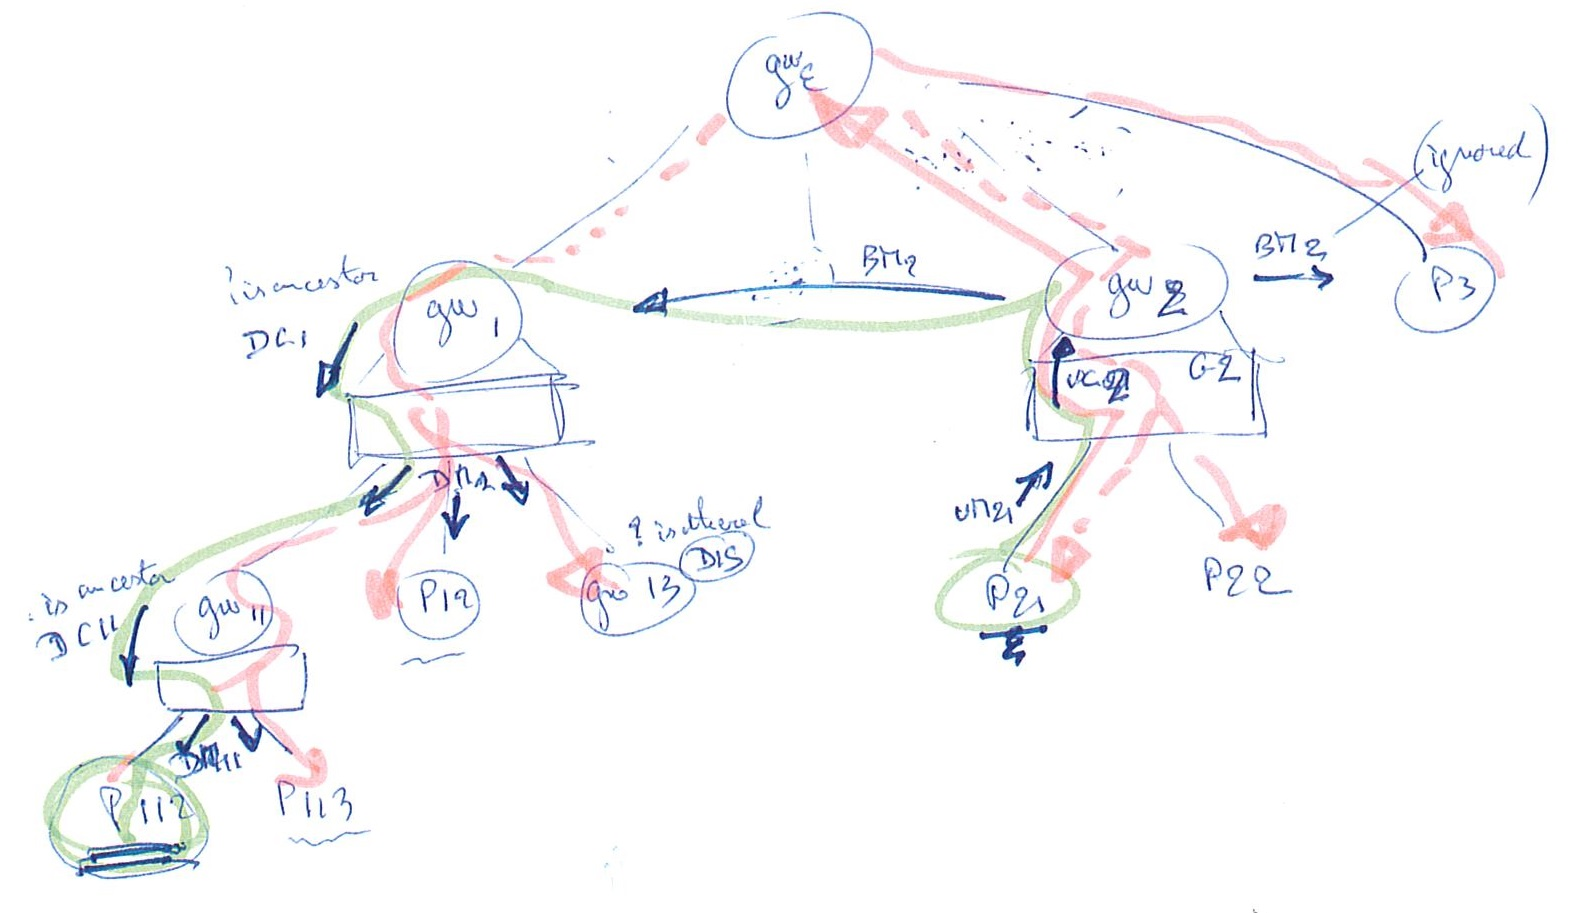
\includegraphics[width=\linewidth]{XFIG/SchemaHB+FB}}
\begin{figure}[h]
%
  \caption{Behaviour of a Gateway Broadcast controller }\label{fig:hb-gatewaybroadcast}
\end{figure}

We will describe the behaviour of the gateways in the next section,
for the different algorithms and variants.

\paragraph{Sort of the processes.}
\label{section:processSort}
The process parameters (the holes of the pNet structure) can emit
messages with a target address as an argument (we abstract away from
any other message content), or receive a message, also with the target
address. But because of the Broadcast mechanism, there are two ways a
process can send messages, either horizontally, broadcasted to all its
siblings, denoted $!bm(t)$, or upward to the next hierarchy level,
denoted $!um(t)$. In the appendix, we
will propose a way to implement this mechanism using a small pNet as a
filter. But from now on, this would complexify the examples, so we
simply assume that the processes have a sort $\{?m(t), !bm(t),
!um(t)\}$. A process is always ready to accept an incoming message,
even if the target argument does not match with its own address. The
filter in the appendix will be in charge of discarding misfit messages.


%\begin{figure}[h]
% \centerline{  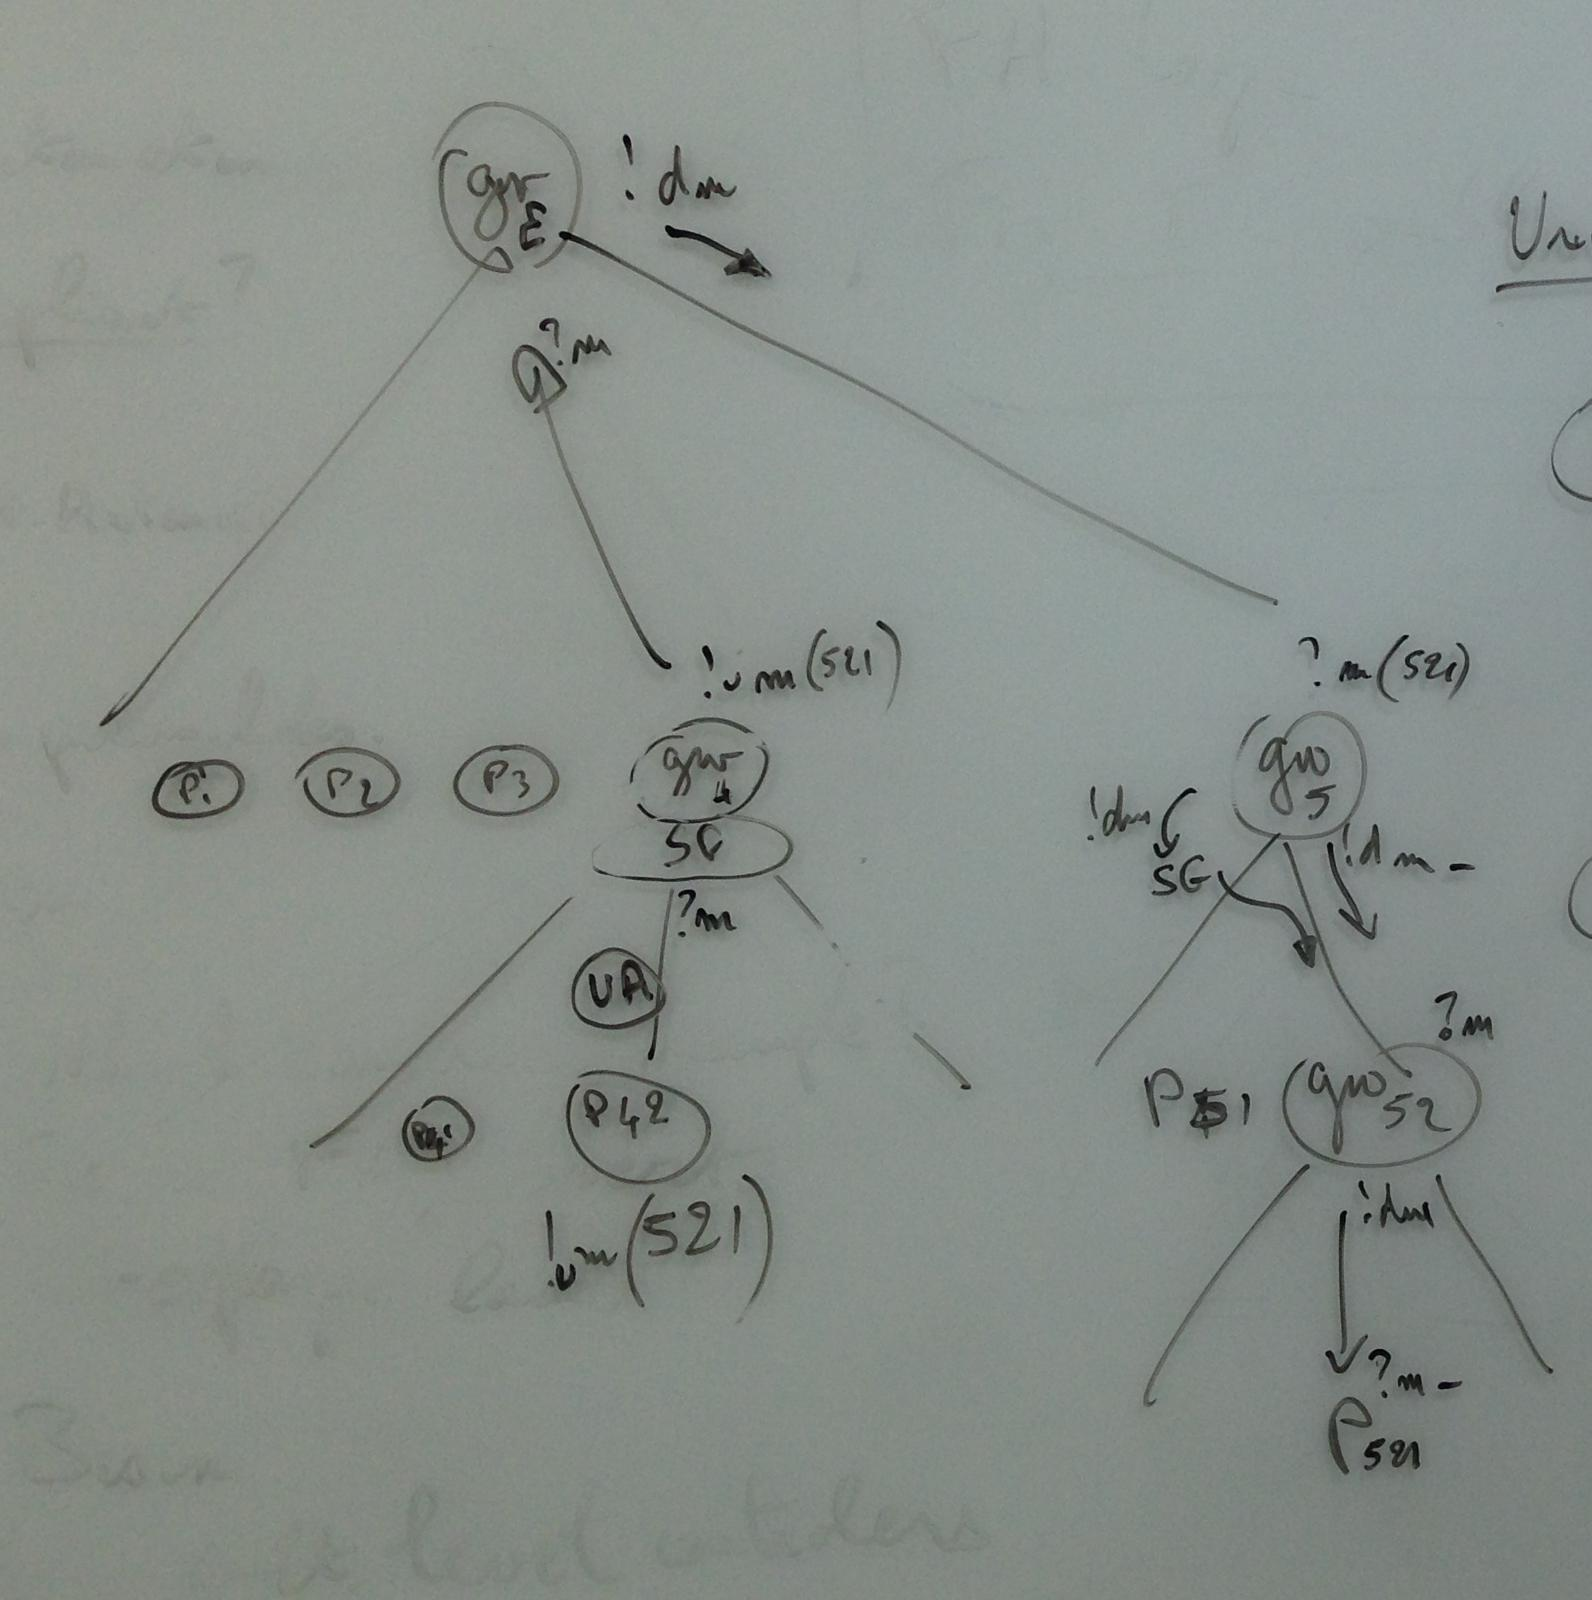
\includegraphics[width=0.7\linewidth]{XFIG/TreeSchema.JPG}}
%  \caption{Structure of hierarchical groups}\label{fig:tree-schema}
% \end{figure}

% \TODO{ To use ?m instead of ?bm} => done.

%% \centerline{  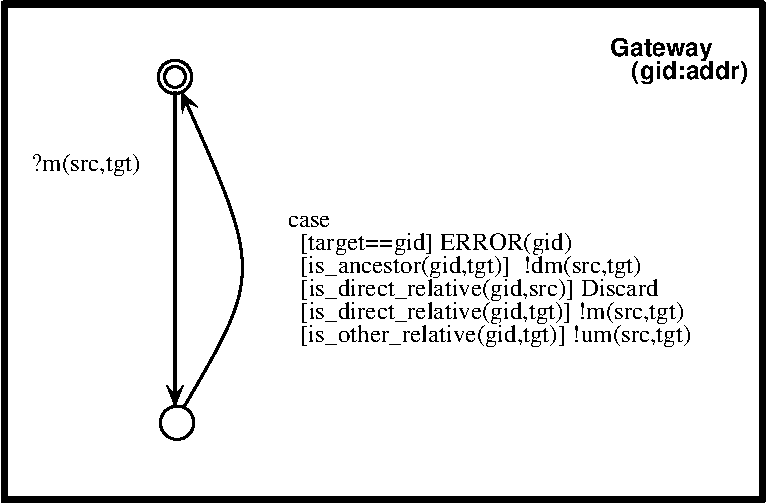
\includegraphics[width=0.6\linewidth]{ATG/Gateway}}
%%   \caption{Bahaviour of a Gateway controller }\label{fig:hb-gateway}
%%  \end{figure}

%% \paragraph{Variant}
%% Another try, with a different message name for sub-group broadcast, so
%% we do not need to pass the src id along... Not sure it makes a simpler
%% model.

%% \begin{figure}[h]

%% \centerline{  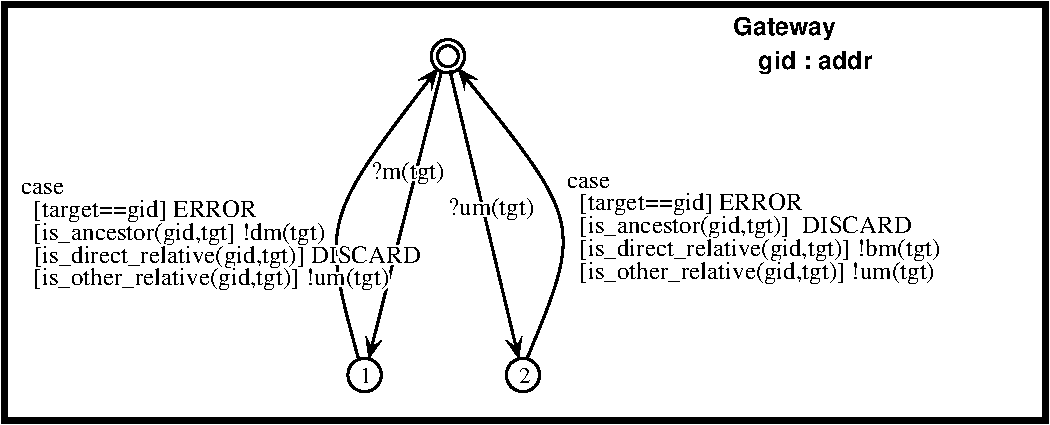
\includegraphics[width=0.8\linewidth]{ATG/Gateway2}}
%%   \caption{Bahaviour of a Gateway HB controller }\label{fig:hb-gateway2}
%%  \end{figure}
%% % \TODO{Eric: to draw the figs of  the broadcast and unicast of
%% % gateway.} done
%% \TODO{Min: to give the formal definition of address and predicates}

%% \begin{figure}[h]
%% \centerline{
%%   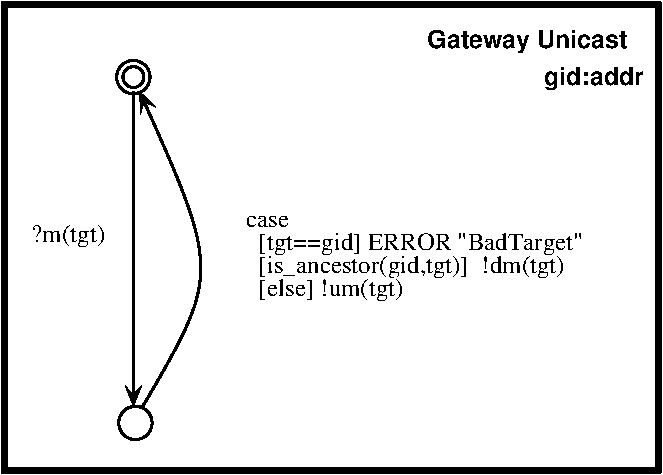
\includegraphics[width=0.5\linewidth]{ATG/GatewayUnicast}
%%   \hspace{10mm}
%%   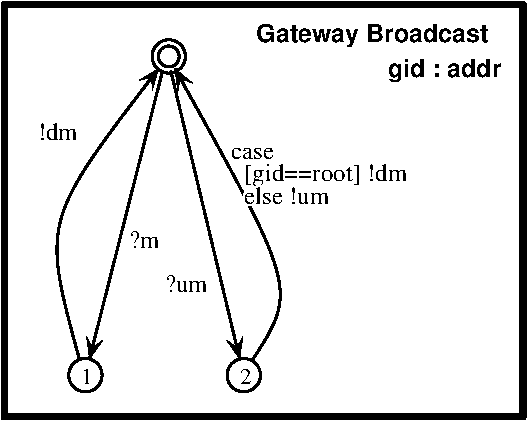
\includegraphics[width=0.4\linewidth]{ATG/GatewayBroadcast}}
%%   \caption{Bahaviour of Unicast and Broadcast gateways}\label{fig:hb-gatewayunicast}
%%  \end{figure}

% \centerline{  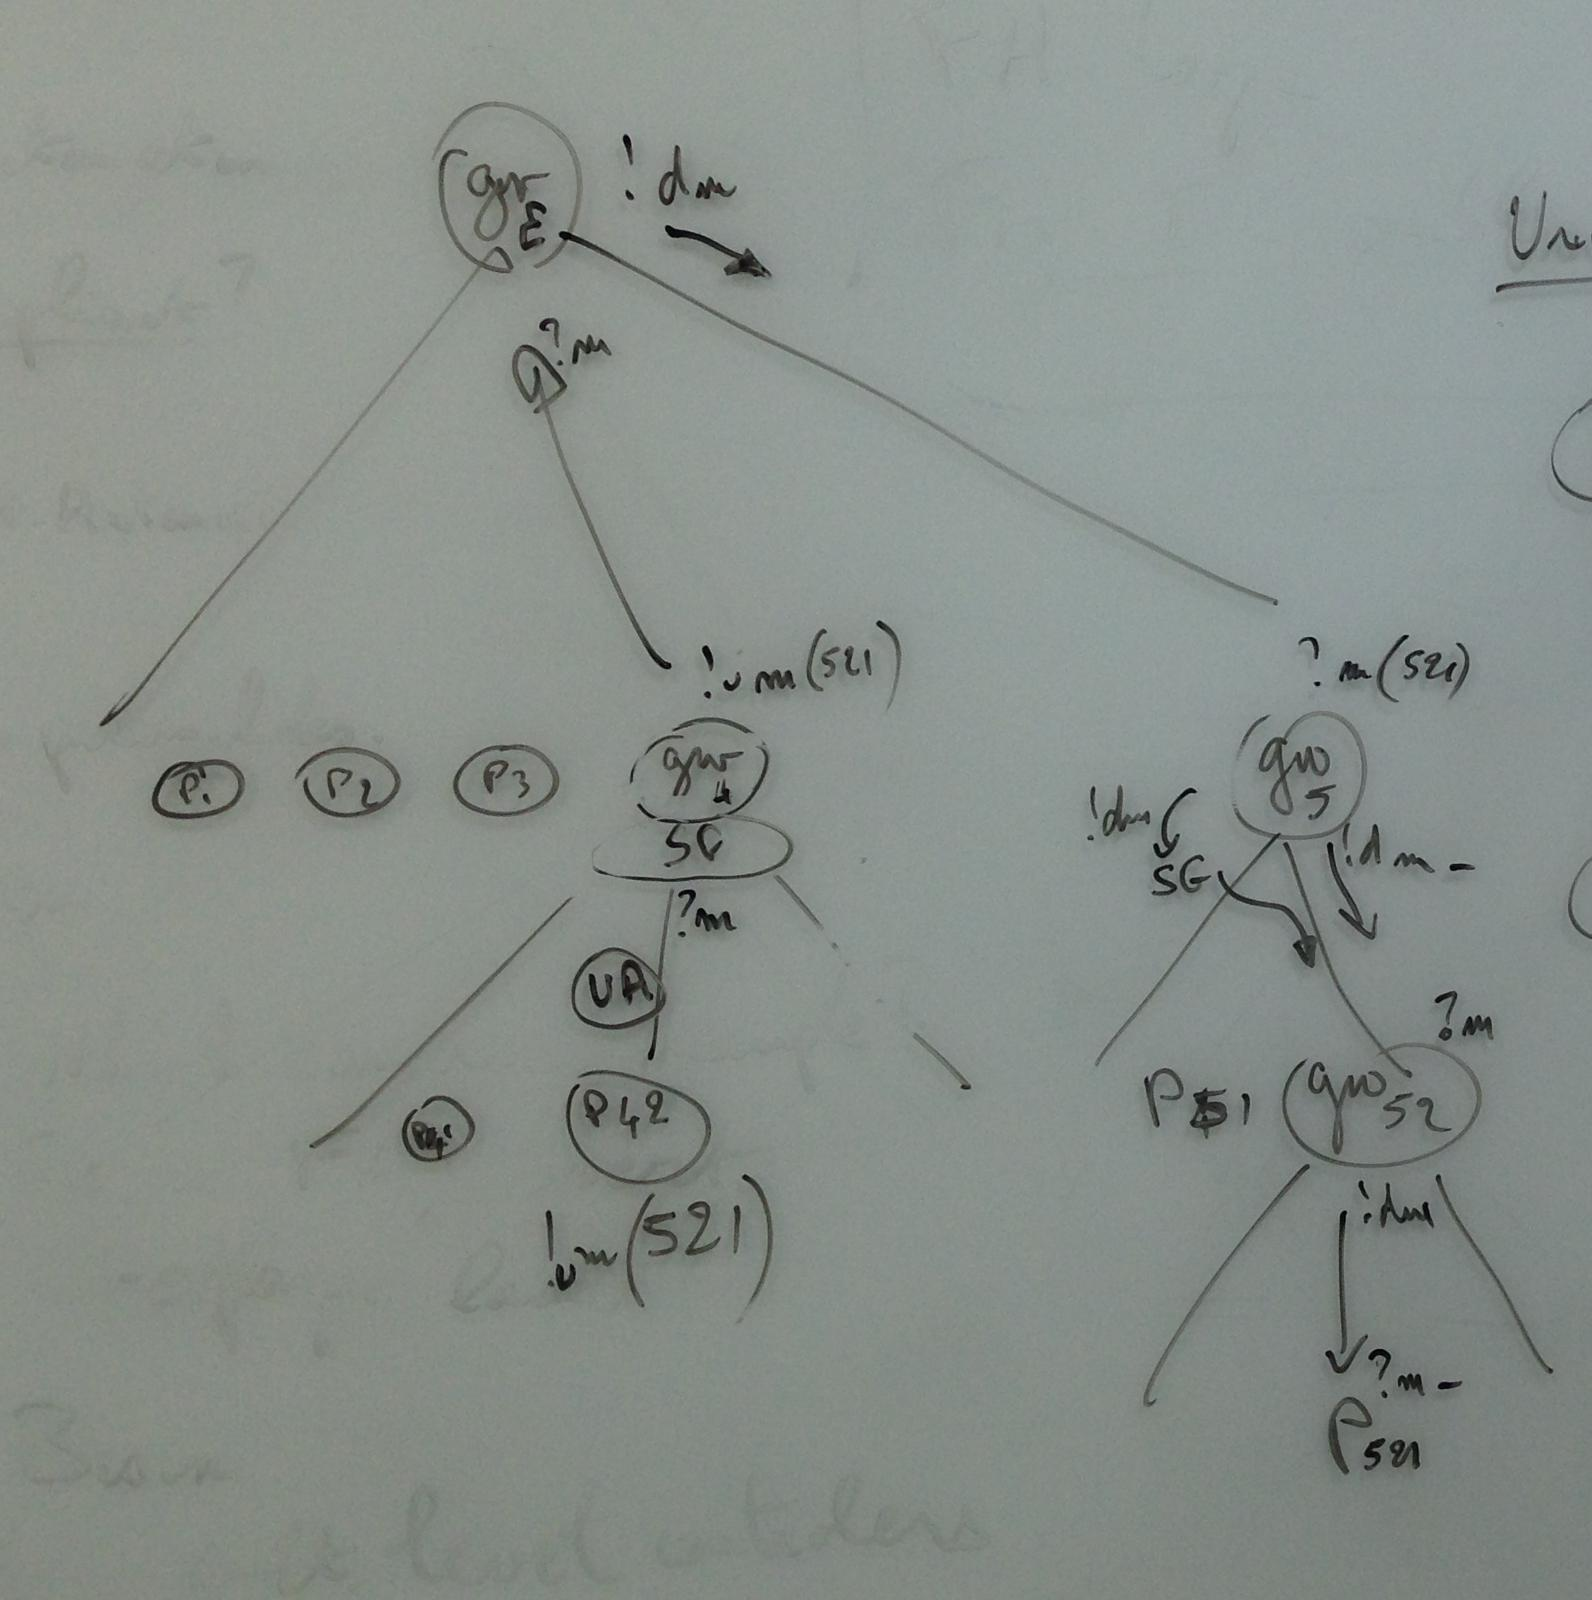
\includegraphics[width=0.7\linewidth]{XFIG/TreeSchema.JPG}}



According to the three algorithms mentioned above, we have three kinds of pNet models for Unicast, Full broadcast and Hierarchical broadcast.

\begin{definition}[B-pNets]\label{B-pNets}
A  broadcasting model is a pNet structure : \\
\centerline{
$B-\pNet\triangleq \mylangle gw_{\widetilde{g}}^{\widetilde{g}\in \widetilde{I_G}},  pc_{\widetilde{p}}^{\widetilde{p}\in \widetilde{I_P}}, sg_{\widetilde{g}}^{\widetilde{g}\in \widetilde{I_G}}, \symb{SV}\myrangle $}
where
\begin{itemize}
\item[$\bullet$] $\widetilde{I_G}$ is the index set over which
  gateways are indexed.  $gw_{\widetilde{g}}^{\widetilde{g}\in
    \widetilde{I_G}}$ is the family of gateways. $\widetilde{I_G}$ is
  also the set over which subgroups are indexed,
  i.e. $gw_{\widetilde{g}}$ links $sg_{\widetilde{g}}$.
   \begin{itemize}
   \item Unicast: $\Sortop (gw_{\widetilde{g}})=\{?m_{\widetilde{g}}(\widetilde{tgt}), 
   !um_{\widetilde{g}}(\widetilde{tgt}),!dm_{\widetilde{g}}(\widetilde{tgt}), ERROR_{g}\}$
   \item Flat Broadcast: $\Sortop 
   (gw_{\widetilde{g}})=\{?m_{\widetilde{g}}(\widetilde{tgt}), 
   !um_{\widetilde{g}}(\widetilde{tgt}),!dm_{\widetilde{g}}(\widetilde{tgt}), 
   ?um_{\widetilde{g}}(\widetilde{tgt})\}$
   \item Hierarchical Broadcast: $\Sortop 
   (gw_{\widetilde{g}})=\{?m_{\widetilde{g}}(\widetilde{tgt}), 
   ?um_{\widetilde{g}}(\widetilde{tgt}), 
   !um_{\widetilde{g}}(\widetilde{tgt}),!dm_{\widetilde{g}}(\widetilde{tgt}), 
   !bm_{\widetilde{g}}(\widetilde{tgt}),DISCARD,
       ERROR_{g}\}$
  \end{itemize}
\item[$\bullet$] $\widetilde{I_P}$ is the index set over which normal
  processes are indexed.
  \item [$\bullet$] $\widetilde{I_{G+P}} \triangleq
    \widetilde{I_G}\uplus\widetilde{I_P}$ is the index set of all
    subnets in a group, i.e. processes and subgroups.
$\widetilde{I_G}$ and $\widetilde{I_P}$ must be \emph{disjoint},
i.e. $\widetilde{I_G}\cap \widetilde{I_P}=\emptyset$. The sort of
$pc_{\widetilde{p}}$ is
\begin{itemize}
\item Unicast: $\Sortop(pc_{\widetilde{p}})=\{!m_{\widetilde{p}}(\widetilde{tgt}),
?m_{\widetilde{p}}(\widetilde{tgt})\}$
\item Flat Broadcast: $\Sortop(pc_{\widetilde{p}})=\{!m_{\widetilde{p}},
?m_{\widetilde{p}}\}$
\item Hierarchical Broadcast: $\Sort(pc_{\widetilde{p}})=\{!um_{\widetilde{p}}(\widetilde{tgt}),
?m_{\widetilde{p}}(\widetilde{tgt}),
!bm_{\widetilde{p}}(\widetilde{tgt})\}$
\end{itemize}

\item[$\bullet$] The subgroup $sg_{\widetilde{g}}$ can be taken the hole of open pNets 
which can be inserted the sub-pNets(subgroups) and has the sort: $\Sortop 
(sg_{\widetilde{g}})=\{?m_{\widetilde{g}}(\widetilde{t}), 
!m_{\widetilde{g}}(\widetilde{t})\}$;

\item[$\bullet$]$\symb{SV}$ is a set of synchronisation vectors. For
  the $HB-\pNet$ node,  we have six kinds of ``normal'' synchronisation
  vectors in the model, plus 2 ``error'' vectors, listed in
  Fig. \ref{fig:HBvectors}.

\end{itemize}
\end{definition}

\centerline{  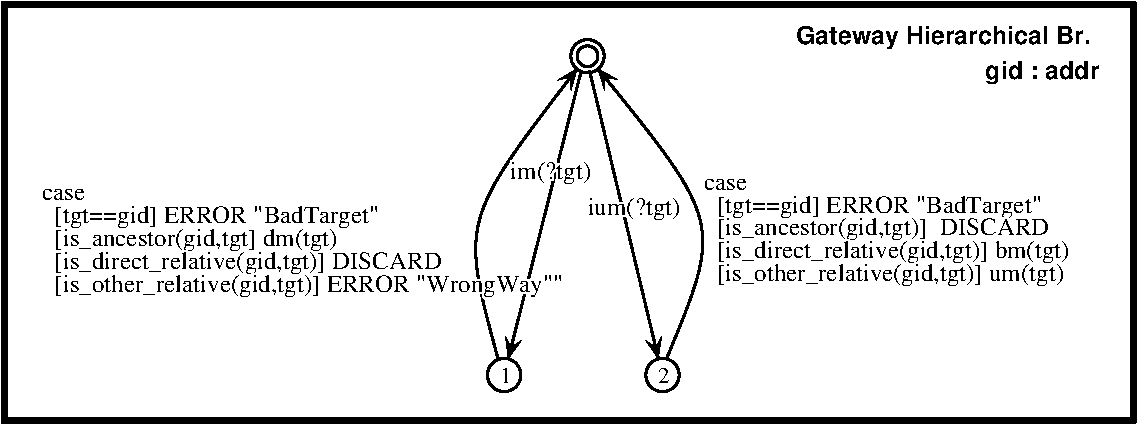
\includegraphics[width=0.85\linewidth]{ATG/GatewayHB}}

\centerline{
   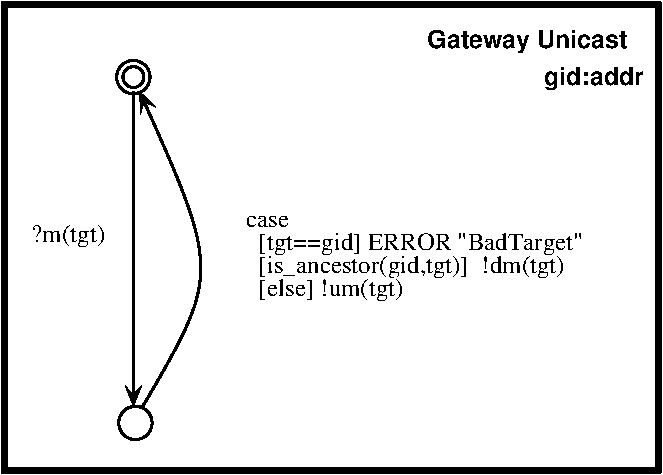
\includegraphics[width=0.5\linewidth]{ATG/GatewayUnicast}
   \hspace{10mm}
   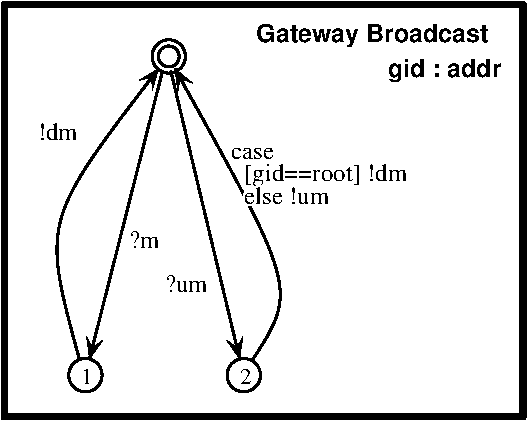
\includegraphics[width=0.4\linewidth]{ATG/GatewayBroadcast}}




%% \vskip 0.5cm
%% \begin{tabular}{|p{2.2cm}|p{9cm}|l|}
%% \hline\hline
%% \multicolumn{3}{|l|}{Full broadcasting}\\
%% \hline
%% $(UC)_{\widetilde{k}}$ & $
%%      \symb{sv}_{u(\widetilde{i}.k)}\triangleq
%%      <?um_{\widetilde{i}.k}(\widetilde{t})\otimes
%%      -^{\widetilde{I_P}}\otimes
%%      !m_{\widetilde{i}.k}(\widetilde{t})\otimes
%%      -^{{\widetilde{I_G}\backslash\{\widetilde{i}\cdot
%%          k\}}}>\longrightarrow \tau(
%%      m_{\widetilde{i}.k}(\widetilde{t}))$ & $\widetilde{k}=\widetilde{i}.k\in \widetilde{I_G}$\\
%% \hline
%% $(DM )_{\widetilde{k}}$& $\symb{sv}_{?\widetilde{i}}\triangleq
%%      <?m_{\widetilde{i}.k}(\widetilde{t})\otimes
%%      -^{\widetilde{I_{G+P}}
%%       \widetilde{I_G}\backslash\{\widetilde{i}\cdot k\}}\otimes -^{\widetilde{I_G}}>\longrightarrow
%%      ?m_{\widetilde{i}}(\widetilde{t})$&$\widetilde{k}=\widetilde{i}.k\in \widetilde{I_G}\uplus \widetilde{I_P}$\\
%%      \hline
%% $(UM)_{\widetilde{k}}$&
%% $\symb{sv}_{!\widetilde{i}}\triangleq
%%     <!um_{\widetilde{i}.k}(\widetilde{t})\otimes
%%     -^{\widetilde{I_P}\uplus
%%       \widetilde{I_G}\backslash\{\widetilde{i}\cdot k\}}\otimes
%%     -^{\widetilde{I_G}}>\longrightarrow
%%     !m_{\widetilde{i}.k}(\widetilde{t})$ & $\widetilde{k}=\widetilde{i}.k\in \widetilde{I_G}\uplus \widetilde{I_P}$\\


%% \hline
%% $(DG )$&
%% $\symb{sv}_{?\widetilde{i}}\triangleq
%%      <?m_{\widetilde{i}.k}^{\forall k\in
%%        I_K}(\widetilde{t})\otimes
%%      -^{\widetilde{I_P}}\otimes -^{\widetilde{I_G}}>\longrightarrow
%%      ?m_{\widetilde{i}}(\widetilde{t})$ & $I_K = \{k/\widetilde{i}.k\in \widetilde{I_G}\uplus
%% \widetilde{I_P}\}$\\

%% \hline\hline
%% \end{tabular}
%% \vskip 0.5cm

%% \begin{tabular}{|p{2.2cm}|p{9cm}|l|}
%% \hline\hline
%% \multicolumn{3}{|l|}{Unicast broadcasting}\\
%% \hline
%% $(UC)_{\widetilde{k}}$ & $
%%      \symb{sv}_{u(\widetilde{i}.k)}\triangleq
%%      <?um_{\widetilde{i}.k}(\widetilde{t})\otimes
%%      -^{\widetilde{I_P}}\otimes
%%      !m_{\widetilde{i}.k}(\widetilde{t})\otimes
%%      -^{{\widetilde{I_G}\backslash\{\widetilde{i}\cdot
%%          k\}}}>\longrightarrow \tau(
%%      m_{\widetilde{i}.k}(\widetilde{t}))$ & $\widetilde{k}=\widetilde{i}.k\in \widetilde{I_G}$\\
%% \hline
%% $(DM )_{\widetilde{k}}$& $\symb{sv}_{?\widetilde{i}}\triangleq
%%      <?m_{\widetilde{i}.k}(\widetilde{t})\otimes
%%      -^{\widetilde{I_P}\uplus
%%       \widetilde{I_G}\backslash\{\widetilde{i}\cdot k\}}\otimes -^{\widetilde{I_G}}>\longrightarrow
%%      ?m_{\widetilde{i}}(\widetilde{t})$&$\widetilde{k}=\widetilde{i}.k\in \widetilde{I_G}\uplus \widetilde{I_P}$\\
%%      \hline
%%      $(UM)_{\widetilde{k}}$&
%% $\symb{sv}_{!\widetilde{i}}\triangleq
%%     <!um_{\widetilde{i}.k}(\widetilde{t})\otimes
%%     -^{\widetilde{I_P}\uplus
%%       \widetilde{I_G}\backslash\{\widetilde{i}\cdot k\}}\otimes
%%     -^{\widetilde{I_G}}>\longrightarrow
%%     !m_{\widetilde{i}.k}(\widetilde{t})$ & $\widetilde{k}=\widetilde{i}.k\in \widetilde{I_G}\uplus \widetilde{I_P}$\\
%% \hline
%% $(DK)_{\widetilde{k}}$&
%% $\symb{sv}_{!\widetilde{i}}\triangleq
%%     <!m_{\widetilde{i}.k}(\widetilde{t})\otimes
%%     ?m_{\widetilde{i}.g}(\widetilde{t})\otimes -^{\widetilde{I_P}\uplus
%%       \widetilde{I_G}\backslash\{\widetilde{i}\cdot k,\widetilde{i}\cdot g\}}\otimes
%%     -^{\widetilde{I_G}}>\longrightarrow
%%     \tau(m_{\widetilde{i}.k}(\widetilde{t}))$ & $\widetilde{k}=\widetilde{i}.k\in \widetilde{I_G}\uplus \widetilde{I_P}$\\

%% \hline\hline
%% \end{tabular}
%\end{definition}

%
%  \begin{itemize}
%  \item[$(BG)_{\widetilde{k}}$]
%    $\symb{sv}_{b(\widetilde{i}.k)}\triangleq
%    <?m_{\widetilde{i}.j}^{\forall j\in I_K}(\widetilde{t})
%    \otimes !bm_{\widetilde{i}.k}(\widetilde{t})
%    \otimes -^{\widetilde{I_G}}>\longrightarrow \tau( bm(\widetilde{t}))$,
%where $I_K = \{k/\widetilde{i}.k\in \widetilde{I_G}\uplus
%\widetilde{I_P}\}$, and $\widetilde{k}=\widetilde{i}.k$
%
%  \item [$(UM)_{\widetilde{k}}$] $
%    \symb{sv}_{!\widetilde{i}}\triangleq
%    <!um_{\widetilde{i}.k}(\widetilde{t})\otimes
%    -^{\widetilde{I_P}\uplus
%      \widetilde{I_G}\backslash\{\widetilde{i}\cdot k\}}\otimes
%    -^{\widetilde{I_G}}>\longrightarrow
%    !m_{\widetilde{i}.k}(\widetilde{t})$,
%where $\widetilde{k}=\widetilde{i}.k\in \widetilde{I_G}\uplus \widetilde{I_P}$;
%
%   \item [$(DC)_{\widetilde{k}}$] $
%     \symb{sv}_{d(\widetilde{i}.k)}\triangleq
%     <!dm_{\widetilde{i}.k}(\widetilde{t})\otimes
%     -^{\widetilde{I_P}}\otimes
%     ?m_{\widetilde{i}.k}(\widetilde{t})\otimes
%     -^{{\widetilde{I_G}\backslash\{\widetilde{i}\cdot k\}}}
%     >\longrightarrow
%     \tau(m_{\widetilde{i}.k}(\widetilde{t}))$,
%where $\widetilde{k}=\widetilde{i}.k\in \widetilde{I_G}$;
%
%   \item [$(UC)_{\widetilde{k}}$] $
%     \symb{sv}_{u(\widetilde{i}.k)}\triangleq
%     <?um_{\widetilde{i}.k}(\widetilde{t})\otimes
%     -^{\widetilde{I_P}}\otimes
%     !m_{\widetilde{i}.k}(\widetilde{t})\otimes
%     -^{{\widetilde{I_G}\backslash\{\widetilde{i}\cdot
%         k\}}}>\longrightarrow \tau(
%     m_{\widetilde{i}.k}(\widetilde{t}))$,
%where $\widetilde{k}=\widetilde{i}.k\in \widetilde{I_G}$;
%
%   \item [$(DG )$] $\symb{sv}_{?\widetilde{i}}\triangleq
%     <?m_{\widetilde{i}.k}^{\forall k\in
%       I_K}(\widetilde{t})\otimes
%     -^{\widetilde{I_P}}\otimes -^{\widetilde{I_G}}>\longrightarrow
%     ?m_{\widetilde{i}}(\widetilde{t})$,
%where $I_K = \{k/\widetilde{i}.k\in \widetilde{I_G}\uplus
%\widetilde{I_P}\}$.
%
% \item [$(DM )_{\widetilde{k}}$] $\symb{sv}_{?\widetilde{i}}\triangleq
%     <?m_{\widetilde{i}.k}(\widetilde{t})\otimes
%     -^{\widetilde{I_P}\uplus
%      \widetilde{I_G}\backslash\{\widetilde{i}\cdot k\}}\otimes -^{\widetilde{I_G}}>\longrightarrow
%     ?m_{\widetilde{i}}(\widetilde{t})$,
%where $\widetilde{k}=\widetilde{i}.k\in \widetilde{I_G}\uplus \widetilde{I_P}$;
%
%\item [$(DIS)_{\widetilde{k}}$] $\symb{sv}_{dc}\triangleq
%     <DISCARD_{\widetilde{i}.k}^{\forall k\in
%       I_K}(\widetilde{t})\otimes
%     -^{\widetilde{I_P}}\otimes -^{\widetilde{I_G}}>\longrightarrow
%     \tau(m_{\widetilde{i}.k}(\widetilde{t}))$,
%where $I_K = \{k/\widetilde{i}.k\in \widetilde{I_G}\uplus
%\widetilde{I_P}\}$.
%\end{itemize}
%\end{itemize}


\medskip

   \begin{example}
We sketch here one example showing how to send one message from one
process in one group to the other process in the other group by using
broadcast mechanism of Hierarchical groups in {\sl HB-pNets}. Here we
use 12, 122,... instead of the denotation above 1.2 , 1.2.2,... in the
definition for short.
   \end{example}

\begin{figure}[h]
  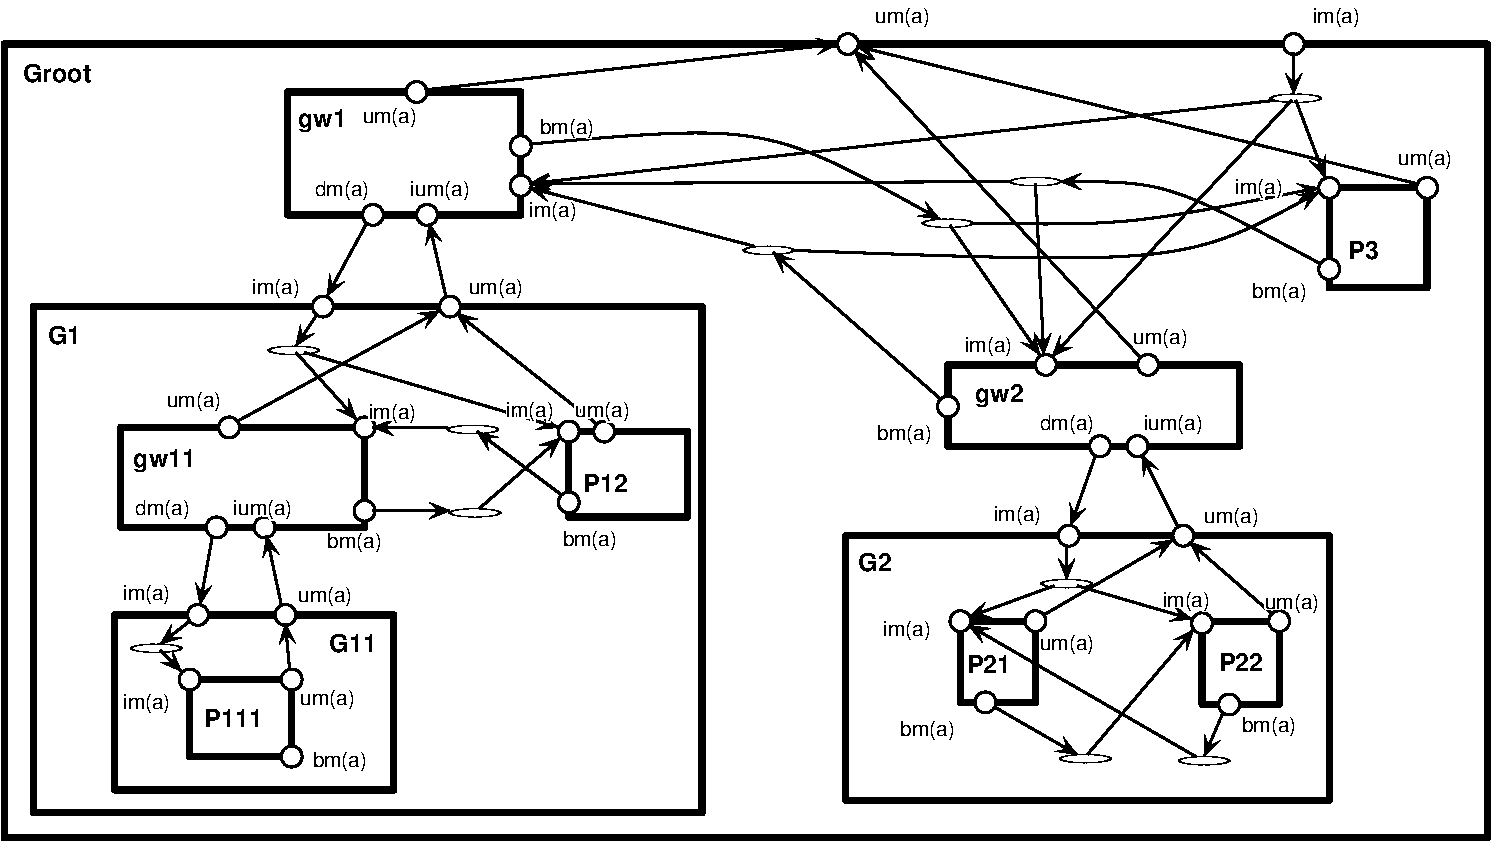
\includegraphics[width=1.0\linewidth]{ATG/Inst5}
  \caption{A Hierarchical Broadcast pNet Structure }\label{fig:hb-structure}
 \end{figure}


In Fig.~\ref{fig:hb-structure}, suppose that one root group $G$ has
  two gateways $g_1$ and $g_2$ which link two subgroups $G_1$ and
  $G_2$, and a normal process $P_3$. Subgroup $G_1$ has one gateway $g_{12}$ which links the
  subsubgroup $G_{12}$ one normal process $P_{12}$.
  $G_2$ and $G_{11}$ have two normal processes respectively.



The procedure of sending one message from process $P_{21}$ to process
$P_{122}$ can be described as follows:

\TODO{To be written, unless it is already in a previous section ?}

\section{Computing the open operational semantics}

In this section we show how to unfold the operational semantic rules
on our hierarchical broadcast example, compute open transitions, and
start building the open automaton.

The sketch we give here considers one particular pNet node, with 2
subgroups, and a specific number of processes in each root- and sub-
groups. Also we make some hypotheses on the sorts of the processes.
Clearly the full proof will have to deal with generalisations of this
particular case.




% \newcommand{\NetS}[1]{\symb{\guillemotleft} #1 \symb{\guillemotright}}

%% A transition in the proof tree is either :
%% \begin{itemize}
%% \item a transition in a pLTS, with eventually a state change.
%% \item an action in the sort of a Hole.
%% \item the ``global action'' resulting from a synchronisation vector in the pNet.
%% \end{itemize}

%% \begin{figure}[h]
%% $\NetS{0_{g1}, 0_{g2}, \sm{P3}, \NetS{0_{g11}, \sm{P12}, \sm{P13},
%%       \sm{SG11}}, \NetS{\sm{P21}, \sm{P22}}}$
%% \hfill
%% $<<0_{g1}, 0_{g2}, 0_{g11}>>$

%% \caption{initial state of our example, and state of the corresponding Expr}
%% \end{figure}


For each possible synch vector of the root node, we build a proof
tree. From each such proof tree we derive a {\em open transition},
representing a symbolic transition in the open automaton
of the pNet.
%% Now we compute the corresponding open-transition, getting rid of the
%% intermediate deduction steps, keeping only premisses for the pLTS
%% and holes involved, and the predicate.

%% \begin{mathpar}
%%   \inferrule
%%       {0_{gw2} \xrightarrow{a_{gw2}} 2_{gw2} \\
%%            \xrightarrow{b_{P21}}
%%            \\ Pred_{Root}
%%       }
%%            {\ostate{000} \xrightarrow{v} \ostate{020}}
%%       ~~ [UG\_2(UM\_21)]
%% \end{mathpar}




\medskip
Following the residual algorithm from section \ref{sec:xxx}, we can
build the full open-automaton of our pNet. We give here in Figure
\ref{fig:xxx} only a small view of its first two states.

\paragraph{Proving equivalences}


We present a (partial) set of transitions of our two processes in the
following tables. For each state of the expression, we have a set of
lines, each defining one open transition starting from this state.
For each specific+ation rule, we show the vectors used to prove it, the
formal hypothesis and the predicte, and the resulting expression
state.


The resulting LTS for our example is shown in Fig. \ref{fig:HB-lts}.


\begin{figure}[h]
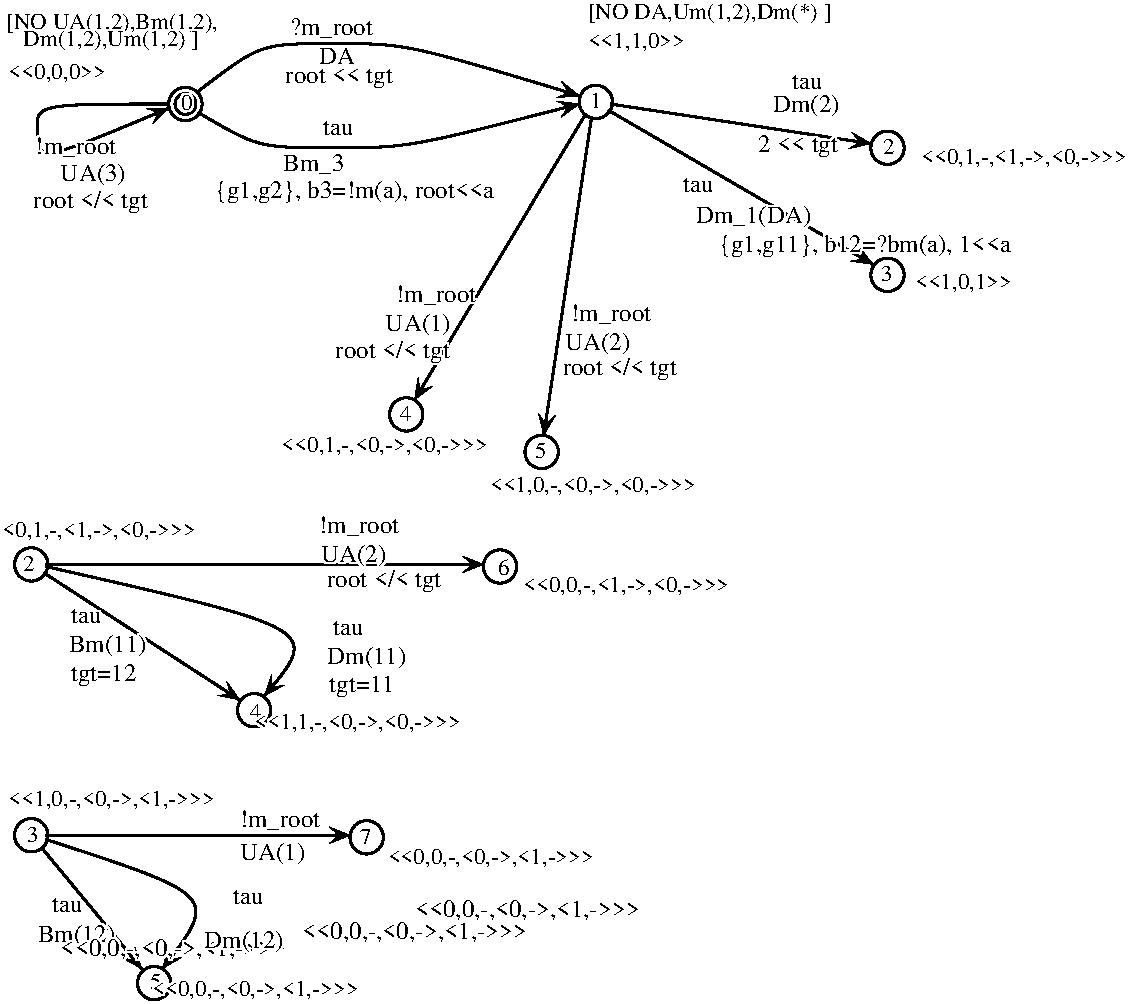
\includegraphics[width=9cm]{ATG/FullLTS}

\caption{(symbolic) behaviour of the example, Hierarchical version}
\label{fig:HB-lts}
\end{figure}

For the flattened version, the computation of the symbolic graph is similar, but of course simpler. The result is shown in Fig. \ref{fig:Flat-lts}.


\begin{figure}[h]
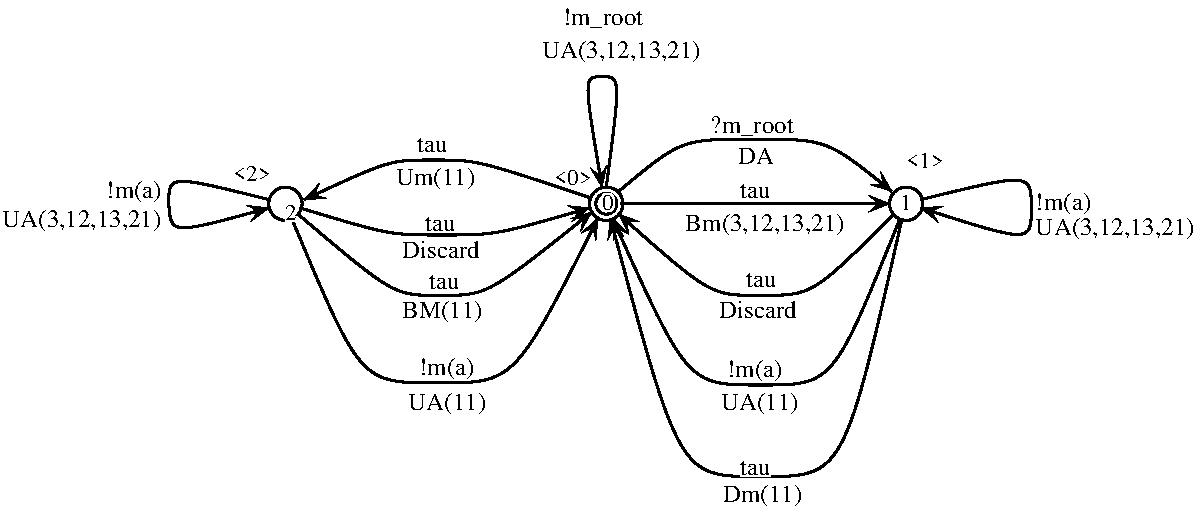
\includegraphics[width=9cm]{ATG/FlatLTS}

\caption{(symbolic) behaviour of the example, Flat version}
\label{fig:Flat-lts}
\end{figure}

%%% REVISION: what we did:
%%% added the notation (x|-> J) page 3 (used to define composition)
%%% defined pnet composiiton (filling a hole)
%%% defined pnests bisimilarity (trivial)
%%% added constraint on synchronisation vector: no fresh variable in target action
%%% changed Pred def: iff instead of implies

